%%%%%%%%%%%%%%%%%%%% book.tex %%%%%%%%%%%%%%%%%%%%%%%%%%%%%
%
% sample root file for the chapters of your "monograph"
%
% Use this file as a template for your own input.
%
%%%%%%%%%%%%%%%% Springer-Verlag %%%%%%%%%%%%%%%%%%%%%%%%%%


% RECOMMENDED %%%%%%%%%%%%%%%%%%%%%%%%%%%%%%%%%%%%%%%%%%%%%%%%%%%
\documentclass[graybox,envcountchap,sectrefs]{svmono}

% choose options for [] as required from the list
% in the Reference Guide

%\usepackage{mathptmx}
%\usepackage{helvet}
%\usepackage{courier}
%

% IMAGES

\usepackage{quiver}

\usepackage{type1cm}         

\usepackage{makeidx}         % allows index generation
\usepackage{graphicx}        % standard LaTeX graphics tool
                             % when including figure files
\usepackage{multicol}        % used for the two-column index
\usepackage[bottom]{footmisc}% places footnotes at page bottom

\usepackage{newtxtext}       % 
\usepackage{newtxmath}       % selects Times Roman as basic font

\usepackage{tikz-cd}
\usepackage{amsmath}
\usepackage{amssymb}

\DeclareFontFamily{U}{mathx}{}
\DeclareFontShape{U}{mathx}{m}{n}{<-> mathx10}{}
\DeclareSymbolFont{mathx}{U}{mathx}{m}{n}
\DeclareMathAccent{\widehat}{0}{mathx}{"70}
\DeclareMathAccent{\widecheck}{0}{mathx}{"71}

\setcounter{tocdepth}{1}     % only include sections, not subsections

\usepackage{hyperref}   % for clickable links
\usepackage{bookmark}   % for improved bookmark organization

\hypersetup{
    colorlinks=true,
    linkcolor=black,     % color of internal links
    citecolor=black,     % color of links to bibliography
    urlcolor=black       % color of external links
}

\usepackage{caption}

\usepackage{ dsfont }

\captionsetup[table]{justification=centering} % Center table captions

% see the list of further useful packages
% in the Reference Guide

\makeindex             % used for the subject index
                       % please use the style svind.ist with
                       % your makeindex program

%%%%%%%%%%%%%%%%%%%%%%%%%%%%%%%%%%%%%%%%%%%%%%%%%%%%%%%%%%%%%%%%%%%%%

\setlength{\parindent}{0pt}
\setlength{\parskip}{0.5\baselineskip}

\graphicspath{{./}{images/}}

\begin{document}

\author{Rutgers University}
\title{Symplectic Summer School 2024}
\subtitle{}

\maketitle

\frontmatter%%%%%%%%%%%%%%%%%%%%%%%%%%%%%%%%%%%%%%%%%%%%%%%%%%%%%%
%%%%%%%%%%%%%%%%%%%%%%acknow.tex%%%%%%%%%%%%%%%%%%%%%%%%%%%%%%%%%%%%%%%%%
% sample acknowledgement chapter
%
% Use this file as a template for your own input.
%
%%%%%%%%%%%%%%%%%%%%%%%% Springer %%%%%%%%%%%%%%%%%%%%%%%%%%

\extrachap{Acknowledgements}

From August 19 to August 23, Rutgers University ran a summer school on symplectic geometry that aimed to provide graduate students and advanced undergraduate students tutorials in various advanced topics in symplectic geometry and introductions to recent developments. This year was focused on, but was not restricted to, the foundational aspects, including the theory of global Kuranishi charts, integer-valued curve-counting invariants, Hamiltonian dynamics, and contact topology.

These notes were scribed by Gary Hu, who is responsible for all mistakes. If you do find any errors, please report them to: gh7@williams.edu

Thanks to Clair Dai and Reyna Li for pointing out errors.

\tableofcontents

\mainmatter%%%%%%%%%%%%%%%%%%%%%%%%%%%%%%%%%%%%%%%%%%%%%%%%%%%%%%%
%%%%%%%%%%%%%%%%%%%%%part.tex%%%%%%%%%%%%%%%%%%%%%%%%%%%%%%%%%%
% 
% sample part title
%
% Use this file as a template for your own input.
%
%%%%%%%%%%%%%%%%%%%%%%%% Springer %%%%%%%%%%%%%%%%%%%%%%%%%%

\begin{partbacktext}
\part{Erkao Bao: Introduction to Contact Homology}

There were three lectures:\\

\begin{enumerate}
    \item \href{#b1}{Day 1: Moduli Spaces of $J$-holomorphic Curves and Compactness}

    In this lecture, we begin with an introduction to basic contact geometry. We then introduce $J$-holomorphic curves as the gradient of the action functional. The focus will be on the moduli space of $J$-holomorphic curves, with a discussion on compactness. We will provide heuristic definitions of cylindrical contact homology and full contact homology.
    
    \item \href{#b2}{Day 2: Cylindrical Contact Homology in Dimension Three via Obstruction Bundle Gluing}

    This lecture addresses the transversality issues associated with the moduli space of $J$-holomorphic curves. We specifically focus on cylindrical contact homology in the 3-dimensional case. The lecture will cover the resolution of transversality issues using obstruction bundle gluing techniques.

    \item \href{#b3}{Day 3: Semi-Global Kuranishi Structure and Full Contact Homology}

    In this lecture, we introduce the semi-global Kuranishi structure. We explore its application in relation to obstruction bundle gluing, including computations of simple examples. The discussion will culminate in the rigorous definition of full contact homology, facilitated by the semi-global Kuranishi structure.

\end{enumerate}

\end{partbacktext}
\chapter{Moduli Spaces of $J$-Holomorphic Curves and Compactness}
\label{b1}
\abstract{In this lecture, we begin with an introduction to basic contact geometry. We then introduce $J$-holomorphic curves as the gradient of the action functional. The focus will be on the moduli space of $J$-holomorphic curves, with a discussion on compactness. We will provide heuristic definitions of cylindrical contact homology and full contact homology.}

\section{Introduction}

\begin{definition}

Let $M^{2n+1}, \xi^{2n}\subset TM$. We say $\xi$ is a \textbf{contact structure} if there exists 1-form $\alpha$ on $M$, called the \textbf{contact form}, such that
\begin{itemize}
\item $\xi = \ker \alpha$
\item $\alpha \wedge (d\alpha)^n \neq 0$
\end{itemize}

\end{definition}

Together, these two conditions imply that $\xi$ is non-integrable.

\begin{example}

$(\mathbb{R}^{2n+1}, \xi_{\text{std}}=\ker \alpha_{\text{std}})$ where
\[
\alpha_{\text{std}}= dz-\sum_{i=1}^n y_i \,dx_i.
\]

When $n=1$, at the origin, we have the contact plane.

\end{example}

\begin{theorem}
[Darboux Theorem]

All contact structures in $\dim 2n+1$ are locally isomorphic.

\end{theorem}

\begin{theorem}
[Gray Stability Theorem]

Consider $\{\xi_t \}_{0\le t \le 1}$ contact structures on $M$. If $M$ is closed, then there exists a 1-parameter family of diffeomorphisms $\phi^t$ of $M$ such that $(\phi^t)_* \xi_t = \xi_0$ where $\phi_0 =\text{id}$.

\end{theorem}

\section{Contact Homology}

Contact homologies are some invariants of contact structures. Before we discuss further, lets look at some applications of contact homologies:

\begin{itemize}
\item \text{[Ustilovsky, 1999]}: $S^{4m+1}$ admits $\infty$ many contact structures in each homotopy class of \textbf{almost contact structures} $(\xi, J, \xi\to \xi, J^2 = -\text{id})$ where $\xi$ is a hyperplane.
\item \text{[Bourgeois, 2004]}: $T^5$ and $T^2 \times S^3$ have $\infty$ contact structures in some homotopy class of almost contact structures.
\item \text{[Giroux, 1994; Eliashberg, Hofer, Givental, 2000]}: On $T^3$, $\alpha = \cos 2\pi n z\,dx + \sin 2\pi n z \,dy$, $\xi_n = \ker \alpha_n$, where $\xi$ are pairwise non-isomorphic.
\end{itemize}

\begin{definition}

Given a contact form $\alpha$, $R_\alpha$ is called a \textbf{Reeb vector field} if
\begin{itemize}
\item $\alpha(R_\alpha)=1$ (positively transverses to $\xi$)
\item $\,d\alpha(R_\alpha, \cdot)=0$ (the flow of $R_\alpha$ preserves $\xi$)
\end{itemize}

\end{definition}

\begin{definition}

Periodic orbits of $R_\alpha$ are called \textbf{Reeb orbits}.

\end{definition}

\begin{conjecture}
[Weinstein Conjecture]

If $M^{2n+1}$ is closed, then for any contact form $\alpha$, there exists at least one Reeb orbit.

\end{conjecture}

\begin{theorem}
[Taubes, 2007]

The Weinstein conjecture holds for $n=1$.

\end{theorem}

\begin{definition}

Let $\gamma$ be a Reeb orbit of period $T$, $\varphi^t $ be a time $t$ flow of $R_\alpha$ We say $\gamma$ is non-degenerate if $\,d\varphi^T : \xi_{\gamma(0)}\to \xi_{\gamma(T)}$ does not have $1$ as an eigenvalue.

\end{definition}

\begin{definition}

Trivialize $(\xi|_\gamma, \,d\alpha)$ symplectically. Then $d\varphi^t$ gives a path of symplectic matrices starting at $\text{id}$. For such a path, we can define an integer, called the \textbf{Conley-Zehnder index} of $\gamma$.

\end{definition}

The general definition is complicated so we will only present simple examples:

\begin{example}

Take $n=1, \dim M=3$.
\begin{itemize}
\item Positive hyperbolic: If the eigenvalues of $d\varphi^T$ are positive real numbers and $d\varphi^t(v)$ winds around the origin $k$ times (where $v$ is an eigenvector), then $\mu_{\text{cz}}=2k$ are negative real numbers.
\item Negative hyperbolic: If $d\varphi^t(v)$ winds around $k+\frac{1}{2}$ times, then $\mu_{\text{cz}}(\gamma)=2k+1$.
\item Elliptic: If the eigenvalues are not real, $d\varphi^t (w)$ where $w \in \xi_{\gamma(0)}$ winds between $k$ and $k+1$ times then $\mu_{\text{cz}}(\gamma)=2k+1$.
\end{itemize}

\end{example}

Consider the actional functional $\mathcal{A}:C^\infty(s^t, M)\to \mathbb{R}, \gamma \mapsto \int_{S^1} \gamma^*(\alpha)$ with Reeb orbits $\text{crit }A$, with a complex structure $J:\xi$ acting on itself with $T^2=-\text{id}$ and $\langle u,v \rangle =d\alpha(u, Tv)$ for any $u,v \in \xi$. Then $\langle \cdot, \cdot \rangle$ defines an inner product which implies
\begin{itemize}
\item $d\alpha(u,v) = \,d\alpha(Ju, Jv)$
\item $d\alpha(u, Ju) >0$ for any $u \neq 0 \in \xi$.
\end{itemize}

Take $\eta_1, \eta_2 \in T_\gamma C^\infty(S^1,M)$ with
\[
\langle \eta_1, \eta_2 \rangle=\int_{S^1} \langle \eta_1, \eta_2 \rangle + \alpha(\eta_1)\alpha(\eta_2)\,dt.
\]

Take $u: \mathbb{R}\to C^\infty(S^1, M)$ with $s\in \mathbb{R}$ and $t\in C^\infty(S^1, M)$ with $\dim u(s)$ are Reeb orbits as $s\to \pm \infty$. Then
\[
\dfrac{du}{ds}=-\text{grad }\mathcal{A}
\]
with $u: \mathbb{R}\times S^1 \to M$. This gives
\[
d(u^*\alpha \cdot j)=0 \\
\pi_\xi u_s + J\pi_\xi u_t =0
\]
where $j$ is a complex structure on $\mathbb{R}\times S^1$.

Let's require $u^*d\alpha \cdot j = da$ where $a: \mathbb{R}\times S^1 \to \mathbb{R}$.  Let $\tilde{u}=(a,u):\mathbb{R}\times S^1 \to \mathbb{R}\times M$. Now, we extend $J$: $T(\mathbb{R}\times M)=\mathbb{R}(\partial a) \oplus \mathbb{R}(R_\alpha)\oplus \xi$ where $a\in \mathbb{R}$, and extend $J: \mathbb{R}(\partial_a)\to \mathbb{R}(R_\alpha)$. $\tilde{u}$ is $J$-holomorphic, i.e.
\[
\overline{\partial}\tilde{u}= \dfrac{1}{2} (d\tilde{u}+J(\tilde{u})d\tilde{u}\cdot j)=0
\]
or
\[
\tilde{u}_s+J(\tilde{u})\tilde{u}_t = 0
\]

Next time, we will study the compactification of moduli spaces of $J$-holomorphic cylinders.
\chapter{Cylindrical Contact Homology in Dimension Three via Obstruction Bundle Gluing}
\label{b2}

\abstract{This lecture addresses the transversality issues associated with the moduli space of $J$-holomorphic curves. We specifically focus on cylindrical contact homology in the 3-dimensional case. The lecture will cover the resolution of transversality issues using obstruction bundle gluing techniques.}
\section{Compactification}

Let $\tilde{\mathcal{M}}(\gamma_+, \gamma_-): \left\{J\text{-holomorphic curves }\mathbb{R}\times S^1 \to \mathbb{R}\times M \right\}/\text{out of domain}$. There are asymptotic markers $\gamma_+$ and $\gamma_-$ on $\mathbb{R}\times M$, and at the points at $\infty$ of $\mathbb{R}\times S^1$ are markers in a way such that markers are mapped to markers. At each embedded Reeb orbit, choose a starting point. Define $\mathcal{M}=\tilde{\mathcal{M}}/\mathbb{R}$, which acts on $\mathbb{R}\times M$ by translation.

A sequence of $J$-holomorphic cylinder can converge to broken ones: we can break a cylinder $\mathbb{R}\times M$ into two cylinders $\mathbb{R}\times M$:

\begin{center}

\tikzset{every picture/.style={line width=0.75pt}} %set default line width to 0.75pt        

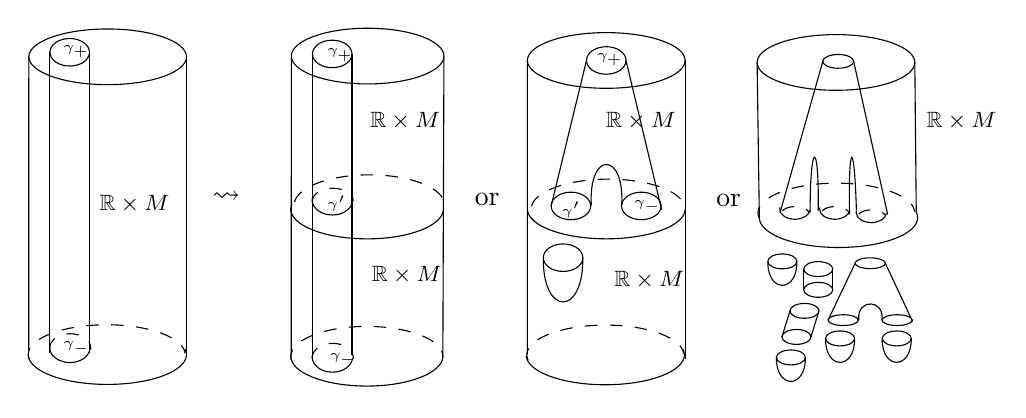
\begin{tikzpicture}[x=0.6pt,y=0.6pt,yscale=-1,xscale=1]
%uncomment if require: \path (0,300); %set diagram left start at 0, and has height of 300

%Shape: Ellipse [id:dp056395190934285244] 
\draw   (30.05,42.21) .. controls (30.05,32.95) and (51.31,25.44) .. (77.54,25.44) .. controls (103.76,25.44) and (125.02,32.95) .. (125.02,42.21) .. controls (125.02,51.48) and (103.76,58.98) .. (77.54,58.98) .. controls (51.31,58.98) and (30.05,51.48) .. (30.05,42.21) -- cycle ;
%Shape: Arc [id:dp6990177911205233] 
\draw  [draw opacity=0] (124.2,218.19) .. controls (124.74,219.28) and (125.02,220.4) .. (125.02,221.54) .. controls (125.02,231.47) and (103.68,239.51) .. (77.36,239.51) .. controls (51.54,239.51) and (30.52,231.77) .. (29.72,222.11) -- (77.36,221.54) -- cycle ; \draw   (124.2,218.19) .. controls (124.74,219.28) and (125.02,220.4) .. (125.02,221.54) .. controls (125.02,231.47) and (103.68,239.51) .. (77.36,239.51) .. controls (51.54,239.51) and (30.52,231.77) .. (29.72,222.11) ;  
%Straight Lines [id:da0017531833743447134] 
\draw    (30.05,41.97) -- (30.01,219.17) ;
%Straight Lines [id:da06191856902561077] 
\draw    (125.02,42.21) -- (125.02,221.93) ;
%Shape: Arc [id:dp7515744636820547] 
\draw  [draw opacity=0][dash pattern={on 4.5pt off 4.5pt}] (30.51,224.86) .. controls (29.98,223.78) and (29.7,222.67) .. (29.7,221.54) .. controls (29.7,211.61) and (50.85,203.57) .. (76.94,203.57) .. controls (102.32,203.57) and (123.02,211.19) .. (124.12,220.74) -- (76.94,221.54) -- cycle ; \draw  [dash pattern={on 4.5pt off 4.5pt}] (30.51,224.86) .. controls (29.98,223.78) and (29.7,222.67) .. (29.7,221.54) .. controls (29.7,211.61) and (50.85,203.57) .. (76.94,203.57) .. controls (102.32,203.57) and (123.02,211.19) .. (124.12,220.74) ;  
%Shape: Ellipse [id:dp170371749578063] 
\draw   (42.78,39.48) .. controls (42.78,34.9) and (48.11,31.19) .. (54.68,31.19) .. controls (61.25,31.19) and (66.58,34.9) .. (66.58,39.48) .. controls (66.58,44.06) and (61.25,47.77) .. (54.68,47.77) .. controls (48.11,47.77) and (42.78,44.06) .. (42.78,39.48) -- cycle ;
%Straight Lines [id:da7961683638948691] 
\draw    (42.78,39.48) -- (42.78,220.58) ;
%Straight Lines [id:da10134655093172151] 
\draw    (66.58,39.48) -- (66.58,220.58) ;
%Shape: Ellipse [id:dp0975147561159333] 
\draw   (188.15,41.77) .. controls (188.15,32.51) and (208.73,25) .. (234.11,25) .. controls (259.48,25) and (280.06,32.51) .. (280.06,41.77) .. controls (280.06,51.04) and (259.48,58.55) .. (234.11,58.55) .. controls (208.73,58.55) and (188.15,51.04) .. (188.15,41.77) -- cycle ;
%Shape: Arc [id:dp3077894307206215] 
\draw  [draw opacity=0] (279.39,222.94) .. controls (278.85,232.68) and (258.56,240.51) .. (233.6,240.51) .. controls (208.31,240.51) and (187.8,232.47) .. (187.8,222.54) .. controls (187.8,221.51) and (188.02,220.51) .. (188.44,219.53) -- (233.6,222.54) -- cycle ; \draw   (279.39,222.94) .. controls (278.85,232.68) and (258.56,240.51) .. (233.6,240.51) .. controls (208.31,240.51) and (187.8,232.47) .. (187.8,222.54) .. controls (187.8,221.51) and (188.02,220.51) .. (188.44,219.53) ;  
%Straight Lines [id:da4345493582140463] 
\draw    (188.15,42.97) -- (188.11,220.17) ;
%Straight Lines [id:da7275152931898132] 
\draw    (280.06,41.77) -- (279.4,223.71) ;
%Shape: Arc [id:dp15000914940586108] 
\draw  [draw opacity=0][dash pattern={on 4.5pt off 4.5pt}] (188.53,225.76) .. controls (188.05,224.72) and (187.8,223.64) .. (187.8,222.54) .. controls (187.8,212.61) and (208.3,204.57) .. (233.6,204.57) .. controls (258.89,204.57) and (279.39,212.61) .. (279.39,222.54) .. controls (279.39,222.67) and (279.39,222.8) .. (279.38,222.92) -- (233.6,222.54) -- cycle ; \draw  [dash pattern={on 4.5pt off 4.5pt}] (188.53,225.76) .. controls (188.05,224.72) and (187.8,223.64) .. (187.8,222.54) .. controls (187.8,212.61) and (208.3,204.57) .. (233.6,204.57) .. controls (258.89,204.57) and (279.39,212.61) .. (279.39,222.54) .. controls (279.39,222.67) and (279.39,222.8) .. (279.38,222.92) ;  
%Shape: Ellipse [id:dp7257031377511021] 
\draw   (200.88,40.48) .. controls (200.88,35.9) and (206.21,32.19) .. (212.78,32.19) .. controls (219.35,32.19) and (224.68,35.9) .. (224.68,40.48) .. controls (224.68,45.06) and (219.35,48.77) .. (212.78,48.77) .. controls (206.21,48.77) and (200.88,45.06) .. (200.88,40.48) -- cycle ;
%Straight Lines [id:da41430031772787657] 
\draw    (200.88,40.48) -- (200.88,221.58) ;
%Straight Lines [id:da8322496496190563] 
\draw    (224.68,40.48) -- (224.68,221.58) ;
%Shape: Arc [id:dp9948607311319655] 
\draw  [draw opacity=0] (279.72,134.27) .. controls (279.18,144.02) and (258.81,151.85) .. (233.76,151.85) .. controls (208.38,151.85) and (187.8,143.81) .. (187.8,133.88) .. controls (187.8,132.85) and (188.02,131.84) .. (188.45,130.86) -- (233.76,133.88) -- cycle ; \draw   (279.72,134.27) .. controls (279.18,144.02) and (258.81,151.85) .. (233.76,151.85) .. controls (208.38,151.85) and (187.8,143.81) .. (187.8,133.88) .. controls (187.8,132.85) and (188.02,131.84) .. (188.45,130.86) ;  
%Shape: Arc [id:dp47440163389587364] 
\draw  [draw opacity=0][dash pattern={on 4.5pt off 4.5pt}] (190.15,129.6) .. controls (192.26,120.45) and (211.6,113.29) .. (235.15,113.29) .. controls (260.12,113.29) and (280.35,121.34) .. (280.35,131.26) .. controls (280.35,132.27) and (280.14,133.26) .. (279.74,134.23) -- (235.15,131.26) -- cycle ; \draw  [dash pattern={on 4.5pt off 4.5pt}] (190.15,129.6) .. controls (192.26,120.45) and (211.6,113.29) .. (235.15,113.29) .. controls (260.12,113.29) and (280.35,121.34) .. (280.35,131.26) .. controls (280.35,132.27) and (280.14,133.26) .. (279.74,134.23) ;  
%Shape: Arc [id:dp6804839012339676] 
\draw  [draw opacity=0] (225.01,223.83) .. controls (224.48,228.48) and (219.25,232.13) .. (212.89,232.13) .. controls (206.17,232.13) and (200.72,228.07) .. (200.72,223.05) .. controls (200.72,222.56) and (200.77,222.07) .. (200.87,221.6) -- (212.89,223.05) -- cycle ; \draw   (225.01,223.83) .. controls (224.48,228.48) and (219.25,232.13) .. (212.89,232.13) .. controls (206.17,232.13) and (200.72,228.07) .. (200.72,223.05) .. controls (200.72,222.56) and (200.77,222.07) .. (200.87,221.6) ;  
%Shape: Arc [id:dp4500398352394417] 
\draw  [draw opacity=0][dash pattern={on 4.5pt off 4.5pt}] (200.83,224.21) .. controls (200.78,223.92) and (200.76,223.62) .. (200.76,223.33) .. controls (200.76,218.61) and (206.29,214.78) .. (213.11,214.78) .. controls (219.93,214.78) and (225.46,218.61) .. (225.46,223.33) .. controls (225.46,223.6) and (225.45,223.88) .. (225.41,224.15) -- (213.11,223.33) -- cycle ; \draw  [dash pattern={on 4.5pt off 4.5pt}] (200.83,224.21) .. controls (200.78,223.92) and (200.76,223.62) .. (200.76,223.33) .. controls (200.76,218.61) and (206.29,214.78) .. (213.11,214.78) .. controls (219.93,214.78) and (225.46,218.61) .. (225.46,223.33) .. controls (225.46,223.6) and (225.45,223.88) .. (225.41,224.15) ;  
%Shape: Arc [id:dp10273519473058612] 
\draw  [draw opacity=0] (224.88,126.86) .. controls (225,127.36) and (225.05,127.88) .. (225.05,128.4) .. controls (225.05,133.42) and (219.61,137.48) .. (212.89,137.48) .. controls (206.17,137.48) and (200.72,133.42) .. (200.72,128.4) .. controls (200.72,127.91) and (200.77,127.42) .. (200.87,126.95) -- (212.89,128.4) -- cycle ; \draw   (224.88,126.86) .. controls (225,127.36) and (225.05,127.88) .. (225.05,128.4) .. controls (225.05,133.42) and (219.61,137.48) .. (212.89,137.48) .. controls (206.17,137.48) and (200.72,133.42) .. (200.72,128.4) .. controls (200.72,127.91) and (200.77,127.42) .. (200.87,126.95) ;  
%Shape: Arc [id:dp9560702304930155] 
\draw  [draw opacity=0][dash pattern={on 4.5pt off 4.5pt}] (200.84,130.15) .. controls (200.79,129.87) and (200.76,129.57) .. (200.76,129.28) .. controls (200.76,124.89) and (206.29,121.33) .. (213.11,121.33) .. controls (219.82,121.33) and (225.28,124.77) .. (225.46,129.06) -- (213.11,129.28) -- cycle ; \draw  [dash pattern={on 4.5pt off 4.5pt}] (200.84,130.15) .. controls (200.79,129.87) and (200.76,129.57) .. (200.76,129.28) .. controls (200.76,124.89) and (206.29,121.33) .. (213.11,121.33) .. controls (219.82,121.33) and (225.28,124.77) .. (225.46,129.06) ;  
%Shape: Arc [id:dp7266228856012471] 
\draw  [draw opacity=0] (66.91,218.04) .. controls (66.38,222.69) and (61.16,226.34) .. (54.79,226.34) .. controls (48.07,226.34) and (42.62,222.27) .. (42.62,217.26) .. controls (42.62,216.76) and (42.67,216.28) .. (42.78,215.81) -- (54.79,217.26) -- cycle ; \draw   (66.91,218.04) .. controls (66.38,222.69) and (61.16,226.34) .. (54.79,226.34) .. controls (48.07,226.34) and (42.62,222.27) .. (42.62,217.26) .. controls (42.62,216.76) and (42.67,216.28) .. (42.78,215.81) ;  
%Shape: Arc [id:dp3689040331833249] 
\draw  [draw opacity=0][dash pattern={on 4.5pt off 4.5pt}] (42.73,218.41) .. controls (42.68,218.12) and (42.66,217.83) .. (42.66,217.53) .. controls (42.66,212.81) and (48.19,208.99) .. (55.01,208.99) .. controls (61.84,208.99) and (67.37,212.81) .. (67.37,217.53) .. controls (67.37,217.81) and (67.35,218.08) .. (67.31,218.35) -- (55.01,217.53) -- cycle ; \draw  [dash pattern={on 4.5pt off 4.5pt}] (42.73,218.41) .. controls (42.68,218.12) and (42.66,217.83) .. (42.66,217.53) .. controls (42.66,212.81) and (48.19,208.99) .. (55.01,208.99) .. controls (61.84,208.99) and (67.37,212.81) .. (67.37,217.53) .. controls (67.37,217.81) and (67.35,218.08) .. (67.31,218.35) ;  
%Shape: Ellipse [id:dp0661139858681199] 
\draw   (330.32,44.41) .. controls (330.32,35.15) and (351.58,27.64) .. (377.81,27.64) .. controls (404.03,27.64) and (425.29,35.15) .. (425.29,44.41) .. controls (425.29,53.67) and (404.03,61.18) .. (377.81,61.18) .. controls (351.58,61.18) and (330.32,53.67) .. (330.32,44.41) -- cycle ;
%Shape: Arc [id:dp8033107315109083] 
\draw  [draw opacity=0] (424.04,218.39) .. controls (424.58,219.47) and (424.87,220.59) .. (424.87,221.74) .. controls (424.87,231.66) and (403.53,239.71) .. (377.21,239.71) .. controls (351.39,239.71) and (330.36,231.97) .. (329.57,222.3) -- (377.21,221.74) -- cycle ; \draw   (424.04,218.39) .. controls (424.58,219.47) and (424.87,220.59) .. (424.87,221.74) .. controls (424.87,231.66) and (403.53,239.71) .. (377.21,239.71) .. controls (351.39,239.71) and (330.36,231.97) .. (329.57,222.3) ;  
%Straight Lines [id:da09066507708598825] 
\draw    (330.32,44.41) -- (330.28,221.6) ;
%Straight Lines [id:da3413965171016031] 
\draw    (425.29,44.41) -- (425.29,224.13) ;
%Shape: Arc [id:dp36547829111768615] 
\draw  [draw opacity=0][dash pattern={on 4.5pt off 4.5pt}] (330.78,225.06) .. controls (330.25,223.98) and (329.97,222.87) .. (329.97,221.74) .. controls (329.97,211.81) and (351.12,203.77) .. (377.21,203.77) .. controls (402.59,203.77) and (423.3,211.38) .. (424.39,220.94) -- (377.21,221.74) -- cycle ; \draw  [dash pattern={on 4.5pt off 4.5pt}] (330.78,225.06) .. controls (330.25,223.98) and (329.97,222.87) .. (329.97,221.74) .. controls (329.97,211.81) and (351.12,203.77) .. (377.21,203.77) .. controls (402.59,203.77) and (423.3,211.38) .. (424.39,220.94) ;  
%Shape: Ellipse [id:dp8629704518272938] 
\draw   (365.91,44.41) .. controls (365.91,39.83) and (371.24,36.12) .. (377.81,36.12) .. controls (384.38,36.12) and (389.71,39.83) .. (389.71,44.41) .. controls (389.71,48.99) and (384.38,52.7) .. (377.81,52.7) .. controls (371.24,52.7) and (365.91,48.99) .. (365.91,44.41) -- cycle ;
%Straight Lines [id:da8452678956957251] 
\draw    (365.91,44.41) -- (344.63,132.03) ;
%Straight Lines [id:da19999367359767395] 
\draw    (389.71,44.41) -- (411.17,134.3) ;
%Curve Lines [id:da16572232996503655] 
\draw    (368.81,131.66) .. controls (366.95,98.15) and (389.34,99.35) .. (387.05,132.03) ;
%Shape: Arc [id:dp6457528380286801] 
\draw  [draw opacity=0] (425.29,134.26) .. controls (424.72,144) and (403.68,151.83) .. (377.8,151.83) .. controls (351.71,151.83) and (330.53,143.87) .. (330.3,134.01) -- (377.8,133.85) -- cycle ; \draw   (425.29,134.26) .. controls (424.72,144) and (403.68,151.83) .. (377.8,151.83) .. controls (351.71,151.83) and (330.53,143.87) .. (330.3,134.01) ;  
%Shape: Arc [id:dp19216152259248287] 
\draw  [draw opacity=0][dash pattern={on 4.5pt off 4.5pt}] (332.81,132.15) .. controls (335.03,123.02) and (354.84,115.88) .. (378.95,115.88) .. controls (403.7,115.88) and (423.92,123.41) .. (425.23,132.88) -- (378.95,133.85) -- cycle ; \draw  [dash pattern={on 4.5pt off 4.5pt}] (332.81,132.15) .. controls (335.03,123.02) and (354.84,115.88) .. (378.95,115.88) .. controls (403.7,115.88) and (423.92,123.41) .. (425.23,132.88) ;  
%Shape: Ellipse [id:dp16448002790374439] 
\draw   (344.63,132.03) .. controls (344.63,127.45) and (349.95,123.74) .. (356.53,123.74) .. controls (363.1,123.74) and (368.43,127.45) .. (368.43,132.03) .. controls (368.43,136.61) and (363.1,140.32) .. (356.53,140.32) .. controls (349.95,140.32) and (344.63,136.61) .. (344.63,132.03) -- cycle ;
%Shape: Ellipse [id:dp9809662464110647] 
\draw   (387.05,132.03) .. controls (387.05,127.45) and (392.37,123.74) .. (398.94,123.74) .. controls (405.52,123.74) and (410.84,127.45) .. (410.84,132.03) .. controls (410.84,136.61) and (405.52,140.32) .. (398.94,140.32) .. controls (392.37,140.32) and (387.05,136.61) .. (387.05,132.03) -- cycle ;
%Shape: Ellipse [id:dp08366558813265468] 
\draw   (339.91,163.18) .. controls (339.91,158.6) and (345.24,154.89) .. (351.81,154.89) .. controls (358.39,154.89) and (363.71,158.6) .. (363.71,163.18) .. controls (363.71,167.76) and (358.39,171.47) .. (351.81,171.47) .. controls (345.24,171.47) and (339.91,167.76) .. (339.91,163.18) -- cycle ;
%Curve Lines [id:da09367632050515562] 
\draw    (339.91,163.18) .. controls (339.4,198.73) and (364.14,198.73) .. (363.71,163.18) ;
%Shape: Ellipse [id:dp8188508828087644] 
\draw   (468.66,45.61) .. controls (468.66,36.34) and (489.92,28.83) .. (516.14,28.83) .. controls (542.37,28.83) and (563.63,36.34) .. (563.63,45.61) .. controls (563.63,54.87) and (542.37,62.38) .. (516.14,62.38) .. controls (489.92,62.38) and (468.66,54.87) .. (468.66,45.61) -- cycle ;
%Shape: Arc [id:dp8117575286418532] 
\draw  [draw opacity=0] (564.51,135.73) .. controls (565.05,136.81) and (565.33,137.93) .. (565.33,139.08) .. controls (565.33,149) and (543.99,157.05) .. (517.67,157.05) .. controls (491.85,157.05) and (470.83,149.31) .. (470.04,139.64) -- (517.67,139.08) -- cycle ; \draw   (564.51,135.73) .. controls (565.05,136.81) and (565.33,137.93) .. (565.33,139.08) .. controls (565.33,149) and (543.99,157.05) .. (517.67,157.05) .. controls (491.85,157.05) and (470.83,149.31) .. (470.04,139.64) ;  
%Straight Lines [id:da331799661099899] 
\draw    (468.66,45.37) -- (470.01,139.6) ;
%Straight Lines [id:da9563297554519652] 
\draw    (563.63,45.61) -- (564.51,135.73) ;
%Shape: Arc [id:dp08014198609210887] 
\draw  [draw opacity=0][dash pattern={on 4.5pt off 4.5pt}] (470.01,139.6) .. controls (469.48,138.52) and (469.21,137.41) .. (469.21,136.28) .. controls (469.21,126.35) and (490.35,118.31) .. (516.44,118.31) .. controls (541.82,118.31) and (562.53,125.92) .. (563.63,135.48) -- (516.44,136.28) -- cycle ; \draw  [dash pattern={on 4.5pt off 4.5pt}] (470.01,139.6) .. controls (469.48,138.52) and (469.21,137.41) .. (469.21,136.28) .. controls (469.21,126.35) and (490.35,118.31) .. (516.44,118.31) .. controls (541.82,118.31) and (562.53,125.92) .. (563.63,135.48) ;  
%Shape: Ellipse [id:dp11318015897818423] 
\draw   (508.22,44.95) .. controls (508.22,42.66) and (512.38,40.81) .. (517.51,40.81) .. controls (522.64,40.81) and (526.8,42.66) .. (526.8,44.95) .. controls (526.8,47.24) and (522.64,49.09) .. (517.51,49.09) .. controls (512.38,49.09) and (508.22,47.24) .. (508.22,44.95) -- cycle ;
%Shape: Arc [id:dp5481702992712509] 
\draw  [draw opacity=0] (546.51,136.57) .. controls (546.06,139.65) and (542.17,142.05) .. (537.43,142.05) .. controls (532.39,142.05) and (528.31,139.34) .. (528.31,135.99) .. controls (528.31,135.62) and (528.36,135.25) .. (528.46,134.9) -- (537.43,135.99) -- cycle ; \draw   (546.51,136.57) .. controls (546.06,139.65) and (542.17,142.05) .. (537.43,142.05) .. controls (532.39,142.05) and (528.31,139.34) .. (528.31,135.99) .. controls (528.31,135.62) and (528.36,135.25) .. (528.46,134.9) ;  
%Shape: Arc [id:dp03984534439684717] 
\draw  [draw opacity=0][dash pattern={on 4.5pt off 4.5pt}] (529.88,136.9) .. controls (531.49,135.39) and (534.33,134.38) .. (537.57,134.38) .. controls (541.2,134.38) and (544.33,135.64) .. (545.79,137.47) -- (537.57,139.78) -- cycle ; \draw  [dash pattern={on 4.5pt off 4.5pt}] (529.88,136.9) .. controls (531.49,135.39) and (534.33,134.38) .. (537.57,134.38) .. controls (541.2,134.38) and (544.33,135.64) .. (545.79,137.47) ;  
%Straight Lines [id:da3617949510353735] 
\draw    (508.22,44.95) -- (482.46,136.1) ;
%Straight Lines [id:da649340590604436] 
\draw    (526.8,44.95) -- (547.3,137.17) ;
%Curve Lines [id:da8727790296078328] 
\draw    (500.59,136) .. controls (500.55,91.73) and (506.07,91.73) .. (505.46,134.9) ;
%Curve Lines [id:da4875409262510293] 
\draw    (524.3,137.17) .. controls (523.55,91.73) and (527.23,91.73) .. (528.46,134.9) ;
%Shape: Ellipse [id:dp7111828464384535] 
\draw   (475.13,165.41) .. controls (475.13,162.93) and (479.04,160.93) .. (483.87,160.93) .. controls (488.7,160.93) and (492.61,162.93) .. (492.61,165.41) .. controls (492.61,167.89) and (488.7,169.89) .. (483.87,169.89) .. controls (479.04,169.89) and (475.13,167.89) .. (475.13,165.41) -- cycle ;
%Curve Lines [id:da9672709945361355] 
\draw    (475.13,165.41) .. controls (474.75,184.63) and (492.92,184.63) .. (492.61,165.41) ;
%Shape: Ellipse [id:dp8770495266103071] 
\draw   (496.76,170.05) .. controls (496.76,167.57) and (500.67,165.56) .. (505.5,165.56) .. controls (510.33,165.56) and (514.24,167.57) .. (514.24,170.05) .. controls (514.24,172.52) and (510.33,174.53) .. (505.5,174.53) .. controls (500.67,174.53) and (496.76,172.52) .. (496.76,170.05) -- cycle ;
%Shape: Ellipse [id:dp4700005658957731] 
\draw   (496.76,182.56) .. controls (496.76,180.08) and (500.67,178.07) .. (505.5,178.07) .. controls (510.33,178.07) and (514.24,180.08) .. (514.24,182.56) .. controls (514.24,185.03) and (510.33,187.04) .. (505.5,187.04) .. controls (500.67,187.04) and (496.76,185.03) .. (496.76,182.56) -- cycle ;
%Shape: Ellipse [id:dp3742015758632733] 
\draw   (488.45,195.21) .. controls (488.45,192.74) and (492.36,190.73) .. (497.19,190.73) .. controls (502.01,190.73) and (505.93,192.74) .. (505.93,195.21) .. controls (505.93,197.69) and (502.01,199.69) .. (497.19,199.69) .. controls (492.36,199.69) and (488.45,197.69) .. (488.45,195.21) -- cycle ;
%Shape: Ellipse [id:dp05712935955362908] 
\draw   (483.6,210.9) .. controls (483.6,208.43) and (487.51,206.42) .. (492.34,206.42) .. controls (497.16,206.42) and (501.08,208.43) .. (501.08,210.9) .. controls (501.08,213.38) and (497.16,215.39) .. (492.34,215.39) .. controls (487.51,215.39) and (483.6,213.38) .. (483.6,210.9) -- cycle ;
%Straight Lines [id:da2384391731418305] 
\draw    (496.76,170.05) -- (496.76,182.56) ;
%Straight Lines [id:da33392656495348927] 
\draw    (514.24,170.05) -- (514.24,182.56) ;
%Straight Lines [id:da566045394847106] 
\draw    (505.93,195.21) -- (501.08,210.9) ;
%Straight Lines [id:da5614446278591068] 
\draw    (488.45,195.21) -- (483.6,210.9) ;
%Shape: Ellipse [id:dp035227786182282506] 
\draw   (480.27,223.26) .. controls (480.27,220.78) and (484.18,218.77) .. (489.01,218.77) .. controls (493.84,218.77) and (497.75,220.78) .. (497.75,223.26) .. controls (497.75,225.73) and (493.84,227.74) .. (489.01,227.74) .. controls (484.18,227.74) and (480.27,225.73) .. (480.27,223.26) -- cycle ;
%Curve Lines [id:da7379429542962657] 
\draw    (480.27,223.26) .. controls (479.89,242.47) and (498.06,242.47) .. (497.75,223.26) ;
%Shape: Ellipse [id:dp5542296065150325] 
\draw   (509.9,211.8) .. controls (509.9,209.33) and (513.82,207.32) .. (518.64,207.32) .. controls (523.47,207.32) and (527.38,209.33) .. (527.38,211.8) .. controls (527.38,214.28) and (523.47,216.29) .. (518.64,216.29) .. controls (513.82,216.29) and (509.9,214.28) .. (509.9,211.8) -- cycle ;
%Curve Lines [id:da7423459609744811] 
\draw    (509.9,211.8) .. controls (509.53,231.02) and (527.7,231.02) .. (527.38,211.8) ;
%Shape: Ellipse [id:dp24342029029087775] 
\draw   (544,211.8) .. controls (544,209.33) and (547.91,207.32) .. (552.74,207.32) .. controls (557.56,207.32) and (561.48,209.33) .. (561.48,211.8) .. controls (561.48,214.28) and (557.56,216.29) .. (552.74,216.29) .. controls (547.91,216.29) and (544,214.28) .. (544,211.8) -- cycle ;
%Curve Lines [id:da21595115366288664] 
\draw    (544,211.8) .. controls (543.62,231.02) and (561.79,231.02) .. (561.48,211.8) ;
%Shape: Ellipse [id:dp9507589820584572] 
\draw   (527.68,166.53) .. controls (527.68,164.74) and (531.76,163.28) .. (536.79,163.28) .. controls (541.82,163.28) and (545.9,164.74) .. (545.9,166.53) .. controls (545.9,168.32) and (541.82,169.77) .. (536.79,169.77) .. controls (531.76,169.77) and (527.68,168.32) .. (527.68,166.53) -- cycle ;
%Straight Lines [id:da7901347005685313] 
\draw    (527.68,166.53) -- (511.39,200.8) ;
%Straight Lines [id:da056288864133154926] 
\draw    (545.9,166.53) -- (562.33,201.69) ;
%Curve Lines [id:da988145377883118] 
\draw    (529.9,200.65) .. controls (528.48,187.55) and (545.61,188.02) .. (543.86,200.8) ;
%Shape: Ellipse [id:dp23604569535188302] 
\draw   (511.39,200.8) .. controls (511.39,199.01) and (515.47,197.55) .. (520.5,197.55) .. controls (525.53,197.55) and (529.61,199.01) .. (529.61,200.8) .. controls (529.61,202.59) and (525.53,204.04) .. (520.5,204.04) .. controls (515.47,204.04) and (511.39,202.59) .. (511.39,200.8) -- cycle ;
%Shape: Ellipse [id:dp7261778653447537] 
\draw   (543.86,200.8) .. controls (543.86,199.01) and (547.94,197.55) .. (552.97,197.55) .. controls (558,197.55) and (562.08,199.01) .. (562.08,200.8) .. controls (562.08,202.59) and (558,204.04) .. (552.97,204.04) .. controls (547.94,204.04) and (543.86,202.59) .. (543.86,200.8) -- cycle ;
%Shape: Arc [id:dp3746223374313047] 
\draw  [draw opacity=0] (524.51,134.57) .. controls (524.06,137.65) and (520.17,140.05) .. (515.43,140.05) .. controls (510.39,140.05) and (506.31,137.34) .. (506.31,133.99) .. controls (506.31,133.62) and (506.36,133.25) .. (506.46,132.9) -- (515.43,133.99) -- cycle ; \draw   (524.51,134.57) .. controls (524.06,137.65) and (520.17,140.05) .. (515.43,140.05) .. controls (510.39,140.05) and (506.31,137.34) .. (506.31,133.99) .. controls (506.31,133.62) and (506.36,133.25) .. (506.46,132.9) ;  
%Shape: Arc [id:dp21450518339030733] 
\draw  [draw opacity=0][dash pattern={on 4.5pt off 4.5pt}] (507.88,134.9) .. controls (509.49,133.39) and (512.33,132.38) .. (515.57,132.38) .. controls (519.2,132.38) and (522.33,133.64) .. (523.79,135.47) -- (515.57,137.78) -- cycle ; \draw  [dash pattern={on 4.5pt off 4.5pt}] (507.88,134.9) .. controls (509.49,133.39) and (512.33,132.38) .. (515.57,132.38) .. controls (519.2,132.38) and (522.33,133.64) .. (523.79,135.47) ;  
%Shape: Arc [id:dp37481817018727304] 
\draw  [draw opacity=0] (500.51,134.57) .. controls (500.06,137.65) and (496.17,140.05) .. (491.43,140.05) .. controls (486.39,140.05) and (482.31,137.34) .. (482.31,133.99) .. controls (482.31,133.62) and (482.36,133.25) .. (482.46,132.9) -- (491.43,133.99) -- cycle ; \draw   (500.51,134.57) .. controls (500.06,137.65) and (496.17,140.05) .. (491.43,140.05) .. controls (486.39,140.05) and (482.31,137.34) .. (482.31,133.99) .. controls (482.31,133.62) and (482.36,133.25) .. (482.46,132.9) ;  
%Shape: Arc [id:dp03724951552805966] 
\draw  [draw opacity=0][dash pattern={on 4.5pt off 4.5pt}] (483.88,134.9) .. controls (485.49,133.39) and (488.33,132.38) .. (491.57,132.38) .. controls (495.2,132.38) and (498.33,133.64) .. (499.79,135.47) -- (491.57,137.78) -- cycle ; \draw  [dash pattern={on 4.5pt off 4.5pt}] (483.88,134.9) .. controls (485.49,133.39) and (488.33,132.38) .. (491.57,132.38) .. controls (495.2,132.38) and (498.33,133.64) .. (499.79,135.47) ;  

% Text Node
\draw (139.08,121.83) node [anchor=north west][inner sep=0.75pt]    {$\rightsquigarrow $};
% Text Node
\draw (71.12,123.83) node [anchor=north west][inner sep=0.75pt]  [font=\footnotesize]  {$\mathbb{R} \times M$};
% Text Node
\draw (208.07,35.68) node [anchor=north west][inner sep=0.75pt]  [font=\tiny]  {$\gamma _{+}$};
% Text Node
\draw (49.15,212.24) node [anchor=north west][inner sep=0.75pt]  [font=\tiny]  {$\gamma _{-}$};
% Text Node
\draw (209.61,219.23) node [anchor=north west][inner sep=0.75pt]  [font=\tiny]  {$\gamma _{-}$};
% Text Node
\draw (208.07,124.24) node [anchor=north west][inner sep=0.75pt]  [font=\tiny]  {$\gamma '$};
% Text Node
\draw (297.07,122.73) node [anchor=north west][inner sep=0.75pt]   [align=left] {or};
% Text Node
\draw (49.15,33.72) node [anchor=north west][inner sep=0.75pt]  [font=\tiny]  {$\gamma _{+}$};
% Text Node
\draw (392.94,127.04) node [anchor=north west][inner sep=0.75pt]  [font=\tiny]  {$\gamma _{-}$};
% Text Node
\draw (349.35,128.14) node [anchor=north west][inner sep=0.75pt]  [font=\tiny]  {$\gamma '$};
% Text Node
\draw (370.56,38.38) node [anchor=north west][inner sep=0.75pt]  [font=\tiny]  {$\gamma _{+}$};
% Text Node
\draw (442.53,123.33) node [anchor=north west][inner sep=0.75pt]   [align=left] {or};
% Text Node
\draw (235.12,166.83) node [anchor=north west][inner sep=0.75pt]  [font=\footnotesize]  {$\mathbb{R} \times M$};
% Text Node
\draw (234.12,73.83) node [anchor=north west][inner sep=0.75pt]  [font=\footnotesize]  {$\mathbb{R} \times M$};
% Text Node
\draw (376.12,73.83) node [anchor=north west][inner sep=0.75pt]  [font=\footnotesize]  {$\mathbb{R} \times M$};
% Text Node
\draw (381.12,169.83) node [anchor=north west][inner sep=0.75pt]  [font=\footnotesize]  {$\mathbb{R} \times M$};
% Text Node
\draw (569.12,73.83) node [anchor=north west][inner sep=0.75pt]  [font=\footnotesize]  {$\mathbb{R} \times M$};


\end{tikzpicture}

\end{center}

where for the rightmost diagram, each of the bottom components is a map to $\mathbb{R}^n$.

\begin{definition}

Let $(F,j)$ be a Riemann surface, $\dot{F}=F$ a finite subset, and $u:(\dot{F},j)\stackrel{J-\text{holomorphic}}{\to} (\mathbb{R}\times M, J)$. Then the \textbf{Hofer energy} is
\[
E(u)=\sup_{\phi \in \mathcal{C}} \int_{\dot{F}} u^* d(\phi, \alpha)
\]
where
\[
\mathcal{C} = \left\{ \phi: \mathbb{R} \to [1,2] \mid
\begin{cases}
\phi(s) = 1 & \text{if } s \ll 0, \\
\phi(s) = 2 & \text{if } s \gg 0, \\
\phi'(s) \ge 0 & \text{for all } s \in \mathbb{R}
\end{cases}
\right\}
\]

\end{definition}

\begin{proposition}

\begin{align*}
E(u)&= 2\sum_{i=1}^{k_+} \mathcal{A}(\gamma_{+,i})-\sum_{i=1}^{k_-} \mathcal{A}(\gamma_{-,i}) \\
&\ge 0.
\end{align*}

\end{proposition}

\section{Grading}

\begin{theorem}

If $u: (\dot{E}, j)\to \mathbb{R}\times M$ is $J$-holomorphic, the following are equivalent:
\begin{itemize}
\item $E(u)<\infty$
\item For any puncture $p$ of $\dot{F}$, either $p$ is removable or $u$ converges to some Reeb orbit along $P$.
\end{itemize}

\end{theorem}

Assume the $H_1(M; \mathbb{Z})$ is torsion free. If $H_1(M)=0$, then for each Reeb orbit $\gamma$, fix a surface $F_\gamma \subset M$ spanning $\gamma$. If $H_1(M; \mathbb{Z})\neq 0$, choose a basis of $H_1(M)$ and represent it by oriented curves $c_1,...c_k$. Choose a trivialization of $\xi/c_1$. For any Reeb orbit $\gamma$, choose $F_\gamma$ such that $[\partial F_\gamma]=[\gamma]-\sum n_i [c_i]$. Choose a trivialization of $\xi \mid_{\gamma}$ so that it extends over $F_\gamma$ and agrees with the trivialization of $\xi/c_i$. This defines a Conley-Zehder index for each $\gamma$.

For each $J$-holomorphic cylinder $u$, we can attach $F_{\gamma_+}$ and $F_{\gamma_-}$:
\begin{center}
\tikzset{every picture/.style={line width=0.75pt}} %set default line width to 0.75pt        

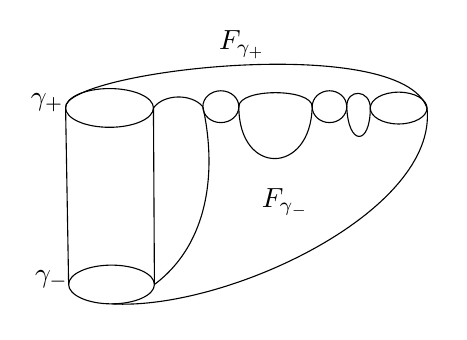
\begin{tikzpicture}[x=0.5pt,y=0.5pt,yscale=-1,xscale=1]
%uncomment if require: \path (0,300); %set diagram left start at 0, and has height of 300

%Shape: Ellipse [id:dp8909013950100437] 
\draw   (85,82) .. controls (85,74.27) and (99.21,68) .. (116.75,68) .. controls (134.29,68) and (148.5,74.27) .. (148.5,82) .. controls (148.5,89.73) and (134.29,96) .. (116.75,96) .. controls (99.21,96) and (85,89.73) .. (85,82) -- cycle ;
%Straight Lines [id:da939999364801372] 
\draw    (85,82) -- (87.2,209.6) ;
%Straight Lines [id:da32030547024849] 
\draw    (148.5,82) -- (149.2,209.6) ;
%Shape: Ellipse [id:dp22593738557210807] 
\draw   (87.2,209.6) .. controls (87.2,201.87) and (101.08,195.6) .. (118.2,195.6) .. controls (135.32,195.6) and (149.2,201.87) .. (149.2,209.6) .. controls (149.2,217.33) and (135.32,223.6) .. (118.2,223.6) .. controls (101.08,223.6) and (87.2,217.33) .. (87.2,209.6) -- cycle ;
%Shape: Ellipse [id:dp3903650035201627] 
\draw   (184.2,81.1) .. controls (184.2,74.75) and (190.02,69.6) .. (197.2,69.6) .. controls (204.38,69.6) and (210.2,74.75) .. (210.2,81.1) .. controls (210.2,87.45) and (204.38,92.6) .. (197.2,92.6) .. controls (190.02,92.6) and (184.2,87.45) .. (184.2,81.1) -- cycle ;
%Shape: Ellipse [id:dp439043297167095] 
\draw   (263.2,81.1) .. controls (263.2,74.75) and (268.8,69.6) .. (275.7,69.6) .. controls (282.6,69.6) and (288.2,74.75) .. (288.2,81.1) .. controls (288.2,87.45) and (282.6,92.6) .. (275.7,92.6) .. controls (268.8,92.6) and (263.2,87.45) .. (263.2,81.1) -- cycle ;
%Shape: Ellipse [id:dp5515211986371753] 
\draw   (305.2,82.1) .. controls (305.2,75.75) and (314.38,70.6) .. (325.7,70.6) .. controls (337.02,70.6) and (346.2,75.75) .. (346.2,82.1) .. controls (346.2,88.45) and (337.02,93.6) .. (325.7,93.6) .. controls (314.38,93.6) and (305.2,88.45) .. (305.2,82.1) -- cycle ;
%Curve Lines [id:da43171084391564163] 
\draw    (118.2,223.6) .. controls (201.2,228.6) and (354.2,156.6) .. (346.2,82.1) ;
%Curve Lines [id:da12535479193092525] 
\draw    (85,82) .. controls (82.2,55.6) and (327.2,26.6) .. (346.2,82.1) ;
%Curve Lines [id:da515259067066461] 
\draw    (288.2,81.1) .. controls (289.2,109.6) and (305.2,109.6) .. (305.2,82.1) ;
%Curve Lines [id:da3208943864453322] 
\draw    (210.2,81.1) .. controls (210.2,131.6) and (262.2,130.6) .. (263.2,81.1) ;
%Curve Lines [id:da7762191468457265] 
\draw    (210.2,81.1) .. controls (210.2,67.6) and (263.2,67.6) .. (263.2,81.1) ;
%Curve Lines [id:da23187615015116236] 
\draw    (288.2,81.1) .. controls (288.2,67.6) and (305.2,68.6) .. (305.2,82.1) ;
%Curve Lines [id:da3836381595978182] 
\draw    (148.5,82) .. controls (156.2,71.6) and (176.2,71.6) .. (184.2,81.1) ;
%Curve Lines [id:da3396096780840039] 
\draw    (149.2,209.6) .. controls (189.2,179.6) and (194.2,126.6) .. (184.2,81.1) ;

% Text Node
\draw (58,69.4) node [anchor=north west][inner sep=0.75pt]    {$\gamma _{+}$};
% Text Node
\draw (61,197.4) node [anchor=north west][inner sep=0.75pt]    {$\gamma _{-}$};
% Text Node
\draw (194,24.4) node [anchor=north west][inner sep=0.75pt]    {$F_{\gamma _{+}}$};
% Text Node
\draw (225,138.4) node [anchor=north west][inner sep=0.75pt]    {$F_{\gamma _{-}}$};

\end{tikzpicture}
\end{center}

which gives an element in $H_2(M)$.

Assume does not exist a contractible Reeb orbits. We define a chain complex $(C_*, \partial)$ where $C_*$ is a free $\mathbb{Q}[H_2(M)]$ module generated by all good Reeb orbits. For each $A\in H_2(M)$, $| A|  = -2 \langle c_1(\xi), A \rangle$, define $\partial_{\gamma_+}= \sum_{\gamma_-, A}\# \mathcal{M}(\gamma_+, \gamma_-, A) e^A \frac{1}{m(\gamma_-)}\gamma_-$ where $m(\gamma_-)$ is the multiplcity of $\gamma_-$. This gives $|\gamma_+| -| \gamma_- | -| A| =1$. Define $| \gamma| =\mu_{c_2}(\gamma)+n-3$.

\begin{definition}

$\gamma$ is \textbf{bad} if $\gamma$ is multiple cover of embedded $\gamma'$ and $\mu_{\text{cz}}(\gamma)-\mu_{\text{cz}}(\gamma')$ is odd.

\end{definition}

\begin{example}

For $\dim \mathcal{M}=3$, $\gamma$ is bad if and only if $\gamma$ is an even multiple cover of a negative hyperbolic one.

\end{example}

If there exists a contractible Reeb orbits:
\vspace{-20pt}
\begin{figure}[htbp]
  \centering
  \includegraphics[width=1\textwidth]{images/bao1.png}
  \label{fig:bi14}
\end{figure}
\vspace{-40pt} % Adjust this value to control the space

This gives the contact homology. One important variant of the contact homology is the (rational) symplectic field theory.

\begin{example}

In $\dim =3$, if $\gamma$ is hyperbolic, then
\[
\mu_{\text{cz}}(\gamma, k) = k \mu_{\text{cz}}(\gamma).
\]

Let $u$ be $J$-holomorphic. If $\text{ind }u = \mu(\gamma_+)-\mu(\gamma)-| A| $. If $u$ is $k$-fold cover of $u'$ and there are no elliptic orbits, then $\text{ind }u = k\cdot \text{ind }u'$.

If $u'$ transverses $\text{ind}$ and $\text{ind } u' \ge 1$, then $\text{ind }u \ge k$. In the definition of $\partial, \text{ind }(u)=1 \implies k=1$.

We can always eliminate elliptic orbits up to any action:
\begin{center}
    
\tikzset{every picture/.style={line width=0.75pt}} %set default line width to 0.75pt        

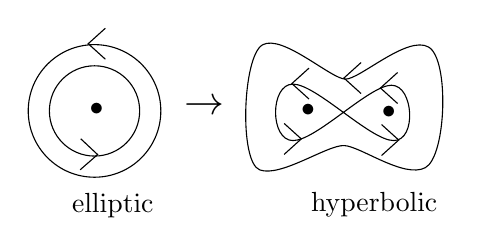
\begin{tikzpicture}[x=0.4pt,y=0.4pt,yscale=-1,xscale=1]
%uncomment if require: \path (0,300); %set diagram left start at 0, and has height of 300

%Shape: Circle [id:dp08144944578189617] 
\draw   (70.82,119.71) .. controls (70.82,86.63) and (97.63,59.82) .. (130.71,59.82) .. controls (163.79,59.82) and (190.6,86.63) .. (190.6,119.71) .. controls (190.6,152.79) and (163.79,179.6) .. (130.71,179.6) .. controls (97.63,179.6) and (70.82,152.79) .. (70.82,119.71) -- cycle ;
%Shape: Circle [id:dp39773554712775216] 
\draw   (89.93,119.71) .. controls (89.93,97.19) and (108.19,78.93) .. (130.71,78.93) .. controls (153.23,78.93) and (171.49,97.19) .. (171.49,119.71) .. controls (171.49,142.23) and (153.23,160.49) .. (130.71,160.49) .. controls (108.19,160.49) and (89.93,142.23) .. (89.93,119.71) -- cycle ;
%Shape: Polygon Curved [id:ds02793189593737866] 
\draw   (399,96.5) .. controls (419,96.5) and (422,146.5) .. (401,146.5) .. controls (380,146.5) and (331,95.5) .. (310,95.5) .. controls (289,95.5) and (289,146.5) .. (310,146.5) .. controls (331,146.5) and (379,96.5) .. (399,96.5) -- cycle ;
%Shape: Polygon Curved [id:ds03073014229495996] 
\draw   (357.5,91) .. controls (370.5,91) and (413.5,51) .. (432.5,62) .. controls (451.5,73) and (448.5,161) .. (429.5,171) .. controls (410.5,181) and (371.5,152) .. (356.5,151) .. controls (341.5,150) and (299,180) .. (280,173) .. controls (261,166) and (264.5,70) .. (282.5,60) .. controls (300.5,50) and (344.5,91) .. (357.5,91) -- cycle ;
\draw   (371.5,104) -- (356,90) -- (371.5,76) ;
\draw   (324.5,109) -- (309,95) -- (324.5,81) ;
\draw   (390,132) -- (405.5,146) -- (390,160) ;
\draw   (302,131) -- (317.5,145) -- (302,159) ;
\draw   (404.5,113) -- (389,99) -- (404.5,85) ;
\draw   (140.5,73) -- (125,59) -- (140.5,45) ;
\draw   (118.25,144.87) -- (133.5,159.14) -- (117.76,172.86) ;

% Text Node
\draw (124,110.4) node [anchor=north west][inner sep=0.75pt]    {$\bullet $};
% Text Node
\draw (315,111.4) node [anchor=north west][inner sep=0.75pt]    {$\bullet $};
% Text Node
\draw (388,113.4) node [anchor=north west][inner sep=0.75pt]    {$\bullet $};
% Text Node
\draw (210,107.4) node [anchor=north west][inner sep=0.75pt]  [font=\Large]  {$\rightarrow $};
% Text Node
\draw (108,192) node [anchor=north west][inner sep=0.75pt]   [align=left] {elliptic};
% Text Node
\draw (324,191) node [anchor=north west][inner sep=0.75pt]   [align=left] {hyperbolic};

\end{tikzpicture}

\end{center}

These two images have the same contact structure, but different contact forms.

\end{example}
\chapter{Semi-Global Kuranishi Structure and Full Contact Homology}
\label{b3}
\abstract{In this lecture, we introduce the semi-global Kuranishi structure. We explore its application in relation to obstruction bundle gluing, including computations of simple examples. The discussion will culminate in the rigorous definition of full contact homology, facilitated by the semi-global Kuranishi structure.}

\section{Introduction}
Suppose $(W,\,d\alpha)$ is an exact symplectic manifold with $\partial W=W_+ + W_-, \alpha|_{W_\pm}=W_{\pm}$, and $J$ an almost complex surface on $\hat{W}$. To count $\text{ind}=0$ $J$-holomorphic cylinders, we obtain a chain map
\[
\Phi: c_*(W_+, \alpha_+, J_+) \to c_*(w_-, \alpha_-, J_-)
\]

Given a 1-parameter family of this data $(W^2, \,d\alpha^2, J^2)$ we want $ \Phi_0 < \Phi_1$ to induce the same map on homology:
\[
\mathcal{M}(\gamma_+, \gamma_-) = \bigsqcup_\iota \{ \iota \}\times \mathcal{M}_{J^2}^{\text{ind}=0} (\gamma_+, \gamma_-).
\]

We want to show that there exists a linear map $K: c_+(W_+, \alpha_+, J_+) \to c_*(W_-, \alpha_-, J_-)$ such that $\Phi_0-\Phi_1 = K\partial + \partial K$.

We have:
\newpage
\vspace{-20pt}
\begin{center}
    \begin{figure}[htbp]
  \centering
  \includegraphics[width=1\textwidth]{images/bao2.png}
  \label{fig:bi14}
\end{figure}
\end{center}
\vspace{-50pt}
For the right most cylinder, we can attach $\mathcal{U}$ to the top half and $\mathcal{M}$ to the bottom half.

For each $\mathcal{U}$, we have a map $\mathcal{S}^{-1}: \mathcal{O}\to [R,\infty)\times M$ and a vector space attached to $\mathcal{O}$ defined by $\ker D_u^*/\mathbb{R} \langle Y \rangle$ where $Y$ comes from variation of $J^2$ and $\mathcal{S}^{-1}(0)$ is the set of curves in $M$ that glue with $\mathcal{U}$.

\section{Semi-Global Kuranishi Structure}

We start with Morse homology case. Let $X$ be a closed manifold, $f: X\to \mathbb{R}$ be a Morse function, $g$ a Riemannian metric, $\phi^t$ the time-$t$ flow of $-\text{grad}_f$, $p\in \text{Crit}(f)$, $\mathcal{D}_p$ be the descending manifold of $p$, and $\mathcal{A}_p$ be the ascending manifold of $p$.

For any $p, q \in \text{Crit}(f)$, 
\[\mathcal{M}(p,q)= \left( \mathcal{A}+q \cap \mathcal{D}_p \right)/\mathbb{R}.
\]

\begin{definition}

An \textbf{interior semi-global Kuranishi chart} is a quadruple $(K, \pi_v: E\to V, \mathcal{L}:V\to E, \psi)$ where
\begin{enumerate}
\item $K\subset M$ is a capacity.
\item $\pi_V: E\to V$ is a finite rank vector bundle of a finite dimensional manifold.
\item $\mathcal{L}$ is a section.
\item $\psi: \mathcal{L}^{-1}(0) \to M$ is homeomorphic onto an open sbuset of $M$ containing $K$.
\item $\dim V - \text{rank} E =\text{vir} \dim\mathcal{M}$
\end{enumerate}

\end{definition}

We order the moduli space $\mathcal{M}_1, \mathcal{M}_2,...$ such that the energy increase. Let
\[
\mathcal{M}_i=\mathcal{M}(p_i, q_i), \qquad E(\mathcal{M}_i)=f(p_i)-f(q_i).
\]
and suppose we have an index tuple $I=(i_1,...,i_n)$ such that $p_{i_m}=q_{i_{m+1}}$. Suppose $S\subset I$ is a subindex tuple. Then $I/S$ is the index tuple obtained by replacing $S$ by an integer which is the index of $\mathcal{M}(p_{s_1}, q_{s_k})$ if $S=(s_1,...,s_k)$, and $\vec{S}\subset I$ is a disjoint union of subindex tuples. We say $I<J$ if there exists $\vec{S} \subset J$ such that $I=J/\vec{S}$.

\begin{definition}

A \textbf{semi-global Kuranishi structure for $\mathcal{M}_1, ..., \mathcal{M}_p$} for any $1\le i \le p$ such that
\begin{enumerate}
\item For each $I$, such that $I/I =i$, $C_I=(\pi_I: E_I \to V_I, \mathcal{L}_: V_I\to E_I, \psi_I: \mathcal{L}_I^{-1}(0) \to M_i )$.
\item For each $I' <I$, we have the restriction inclusion: for $V_{I'I} \subset V_{I'}$ open, we have
   \[\begin{tikzcd}
	& {E_{I'}|_{V_{I'I}}} && {E_I} \\
	\\
	{V_{I'}} & {V_{I'I}} && {V_I}
	\arrow["{{\phi_{I'I}^\#}}", from=1-2, to=1-4]
	\arrow[from=1-2, to=3-2]
	\arrow[from=1-4, to=3-4]
	\arrow["\supset"{description}, draw=none, from=3-1, to=3-2]
	\arrow["{{\mathcal{L}_{I'}}}", curve={height=-18pt}, from=3-2, to=1-2]
	\arrow["{{\phi_{II'}}}", hook, from=3-2, to=3-4]
	\arrow["{{\mathcal{L}_I}}"', curve={height=18pt}, from=3-4, to=1-4]
\end{tikzcd}\]
where the top map is injective and the bottom map is an embedding
\item $\mathcal{L}_I \circ \phi_{I' I} = \phi^\#_{I'I} \mathcal{L}_{I'}|_{V_{II'}}$
\item $(\mathcal{L}_I)_*$ descends to an isomorphism:
        \[
        (\mathcal{L})_I : TV_I/TV_{I\cdot I} \stackrel{\cong}{\longrightarrow} E_I/E_I
        \]
\item Composition of $(\phi_{I'I}, \phi^\#)$ is associative
\item $\mathcal{M}_i = \bigcup_{I, I/I = i} \psi_I(\mathcal{L}_I^{-1}(0))$
\end{enumerate}

\end{definition}

\section{Strata Compatibility}

\begin{definition}

For $I=(i_1,...,i_m)$ define
\begin{align*}
\mathbb{V}_I&=V_{i_1}\times ... \times V_{i_m} \times [R, \infty)^{m-1}, \\
\mathbb{E}_I &= E_{i_1} \oplus ... \oplus E_{i_m}.
\end{align*}
Suppose that $G_I$ a diffeomorphism onto its image, $G_I^\#$ a bundle isomorphism, and $\mathcal{L}_I$ are $C'$-close as $T_1,....,T_{m-1}\to \infty$.

For all $i$, a bundle map satisfies the \textbf{strata compatibility} conditions if the following map commutes
\[\begin{tikzcd}
	{\mathbb{E}_I} && {E_I} \\
	\\
	{\mathbb{V}_I} && {V_I}
	\arrow["{G_I^\#}", from=1-1, to=1-3]
	\arrow[from=1-1, to=3-1]
	\arrow[from=1-3, to=3-3]
	\arrow["{(\mathcal{L}_1, \mathcal{L}_2,..., \mathcal{L}_m)}", curve={height=-18pt}, from=3-1, to=1-1]
	\arrow["{G_I}"', from=3-1, to=3-3]
	\arrow["{{\mathcal{L}_I}}"', curve={height=18pt}, from=3-3, to=1-3]
\end{tikzcd}\]
\end{definition}

Here, the perturbation section is 
\[
\sigma=\left\{G_I: V_I\to F_I \mid I/I = i \right\}
\]
where $\sigma_I$ transverses $\mathcal{L}_I$, $\sigma_I$ is small, the section is compatible with $(\phi_{I'I},\phi_{I'I}^\#)$, and both $\sigma_I$ and $(\sigma_{i_1,i_2,...,i_n})$ are $C^1$-close as $T_1,...,T_{n-1}\to \infty$.

The perturbed moduli space is
\[
Z_i = \coprod_{I/I=i} \mathcal{L}_I^{-1}(\sigma_I)/\sim
\]

\section{Construction of Semi-Global Kuranishi Structures for Cylindrical Contact Homology}

Suppose we have an interior chart $\mathcal{E}\to \mathcal{B}$ and $\overline{\partial}$ on the inverse.

\begin{theorem}

Given any compact $K\subset \mathcal{M}$, there exists an integer and a neighborhood $N(K)\subset B$ and a rank $\ell$ sub-bundle $E\subset \mathcal{E}$ defined over $N(K)$ such that $\overline{\partial}$ transverses $E$ over $N(K)$.

\end{theorem}

\begin{proof}
Pick $\epsilon \gg 0$ small. Find $s_0 \in \mathbb{R}$ such that $\mathcal{A}(u(s-s_0))= \mathcal{A}(\gamma_+)-\epsilon$. Choose $J$ such that $\overline{\partial}_J u = \partial_S u+Au=0$ (where $A$ is a linear self-adjoint operator) is a linear near $\infty$.
\end{proof}

Let $f_i, \lambda_i$ be eigenvectors and eigenvalues of $A$ ordered such that $\lambda_{-2} \le \lambda_{-1} < 0 < \lambda_1\le \lambda_2 \le ...$ and consider
\[
\tilde{f}_j(s,t)=\beta(s)f_k(t)\otimes (\,ds -i\,dt).
\]

Then let $E=\text{span}\{\tilde{f}_1,...,\tilde{f}_\ell\}$. The claim is that $E$ transverses $\overline{\partial}$.  we have $V=\overline{\partial}^{-1}(E)$.

This involves proving the following diagram commutes:

\[\begin{tikzcd}
	{\mathcal{O}_+\oplus \mathcal{O}_-} &&& {\mathcal{O}_{+-}} \\
	\\
	{\mathcal{M}_+ \times \mathcal{M}_- \times [\mathbb{R}, \infty)} &&& V
	\arrow["{G_\#}"', from=1-1, to=1-4]
	\arrow[from=1-1, to=3-1]
	\arrow[from=1-4, to=3-4]
	\arrow["{(0,0)}", curve={height=-24pt}, from=3-1, to=1-1]
	\arrow["G"', from=3-1, to=3-4]
	\arrow["{\mathcal{L}}"', curve={height=18pt}, from=3-4, to=1-4]
\end{tikzcd}\]

%%%%%%%%%%%%%%%%%%%%%part.tex%%%%%%%%%%%%%%%%%%%%%%%%%%%%%%%%%%
% 
% sample part title
%
% Use this file as a template for your own input.
%
%%%%%%%%%%%%%%%%%%%%%%%% Springer %%%%%%%%%%%%%%%%%%%%%%%%%%

\begin{partbacktext}
\part{Mike Usher: Quantitative Symplectic Geometry}

There were three lectures:\\

\begin{enumerate}

    \item \href{#u1}{Day 1: Symplectic Embedding Obstructions and Constructions}

    The question of which subsets of $\mathbb{R}^{2n}$ embed symplectically into which others has turned out to be quite rich and has led to the development of many techniques over the past 40 years. In my first lecture, I will explain proofs of classic results of Gromov that give obstructions to symplectic squeezing and packing, and will contrast this with cases where an explicit construction allows one to give a non-obvious positive answer to a symplectic embedding question.

    \item \href{#u2}{Day 2: Capacities and Symplectic Homology}

    The second lecture will formally introduce the notion of a symplectic capacity, and will discuss two examples of these: the Hofer-Zehnder capacity based on periodic orbits of Hamiltonian systems, and the Floer-Hofer-Wysocki capacity based on symplectic homology.
    
    \item \href{#u3}{Day 3: Obstructing Embeddings Using Equivariant Symplectic Homology}

    The third lecture will explain how $S^1$-equivariant symplectic homology supplies additional restrictions on symplectic embeddings, both via a sequence of capacities coming from spectral invariants associated to various homology classes, and via chain-level information that vanishes in homology but can in some cases be used to show that two known embeddings are not symplectically isotopic.

\end{enumerate}

\end{partbacktext}
\chapter{Symplectic Embedding Obstructions and Constructions}
\label{u1}

\abstract{The question of which subsets of $\mathbb{R}^{2n}$ embed symplectically into which others has turned out to be quite rich and has led to the development of many techniques over the past 40 years. In my first lecture, I will explain proofs of classic results of Gromov that give obstructions to symplectic squeezing and packing, and will contrast this with cases where an explicit construction allows one to give a non-obvious positive answer to a symplectic embedding question.}
\section{Introduction}

Here are some examples of questions that symplectic geometers care about:
\begin{enumerate}
\item Suppose $X(\vec{r})$ and $Y(\vec{s})$ are symplectic manifolds depending on parameters $\vec{r}$ and $\vec{s}$. For what values of $\vec{r}$ and $\vec{s}$ do there exist symplectic embeddings $X(\vec{r})\hookrightarrow Y(\vec{s})$?  For example, do there exist symplectic embeddings $X(\vec{r})\hookrightarrow Y(\vec{s})$ where
\[
    X(\vec{r}) = X(a)=B^{2n}(a)=\left\{ (\vec{x}, \vec{y})\in \mathbb{R}^{2n} \mid  \pi \sum(x_j^2+y_j^2) \le a \right\}
\]
\[
    Y(\vec{s}) = E^{2n}(s_1,...,s_n) = \left\{ (\vec{x}, \vec{y}) \in \mathbb{R}^{2n} \mid  \pi \sum \dfrac{(x_j^2+y_j^2)}{s_j}\le 1 \right\}
\]
with $a>0$?
\item If $X\subset \mathbb{R}^{2n}$ is a domain with contact type boundary, what can be said about the action of closed characteristics on $\partial X$? What is the connection between this question and the previous one?
\item For $\phi: M\to M$ a Hamiltonian diffeomorphism, what happens to the actions of fixed points of $\phi^k$, denoted $\# \text{Fix}\left(\phi^k\right)$, and the Hofer norm $\mid \mid \phi^k\mid \mid_{\text{Hofer}}$ as $k\to \infty$?
\end{enumerate}

For the rest of this talk, we will mostly focus on the first question, partially because the first result that got mathematicians interested in studying quantitative symplectic geometry arose from this problem.

\begin{theorem}
[Gromov's Non-Squeezing Theorem, 1985]

Let
\[
B^{2n}(a) = \left\{ (\vec{x}, \vec{y}) \in \mathbb{R}^{2n} \mid  \pi \sum (x_j^2+y_j^2) \le a\right\}
\]
and
\[
Z^{2n}(A) = \left\{ (\vec{x}, \vec{y}) \in \mathbb{R}^{2n} \mid  \pi(x_j^2+y_j^2) \le A \right\}=B^2(A) \times \mathbb{R}^{2n-2}.
\]
Then there exists a symplectic embedding $B^{2n}(a) \hookrightarrow Z^{2n}(A)$ only if $a\le A$.

\end{theorem}

Basically, this result tells us that we cannot squeeze a ball into a cylinder of smaller radius while preserving the symplectic structure.

\section{Proof of Gromov's Non-Squeezing Theorem}

We present a proof sketch.

Suppose there exists a symplectic embedding $\phi: B^{2n}(a) \hookrightarrow Z^{2n}(A)$. Let $\epsilon >0$. We want to show that $a\le A$, so it suffices to show that $a-\epsilon < A+\epsilon$.

Choose $L$ such that $\text{Im}(\phi) \subset B^2(A)\times (-L,L)^{2n-2}$. Regard $B^2(A)$ as a subset of $S^2(A+\epsilon)$, the 2-sphere with area $A+\epsilon$. Then $\phi$ can be regarded as having image in $(M, \omega)=(S^2(A+\epsilon)\times \mathbb{R}^{2n}/2L\mathbb{Z}^{2n-2})$ with symplectic form $\omega_{\text{std}}\oplus \omega_{\text{std}}$.

There are 2 key facts:

\begin{enumerate}
\item For any $\omega$-compatible almost complex structure $J$ on $M$, there exists a $J$-holomorphic map $u:S^2 \to M$ such that $\phi\left(\vec{0}\right)\subset \text{Im}(u)$ and $u_*[S^2]=[S^2\times \{\text{pts}\}] \in H_c(M)$. In particular, this applies to $J$'s agreeing on $\phi(B^{2n}(a-\frac{\epsilon}{2}))$ with $\phi_*J_0$, where $J_0$ is the standard complex structure on $B^{2n}(u-\frac{\epsilon}{2})$.
\item For a $J_0$-holomorphic map $v: \sum \to B^{2n}(c)$ where $\sum$ is a compact surface with boundary and $c \in (a - \epsilon, a - \frac{\epsilon}{2})$ such that $v(\partial \sum) \subset \partial B^{2n}(c)$ and $\vec{0} \subset \text{Im}(v)$, then $\text{Area}(v) \ge c$.
\end{enumerate}

Together, these two facts prove the desired claim: assuming we have both key facts, for generic $c \in (a-\frac{\epsilon}{2}, a-\epsilon)$, take $\sum u^{-1}(\phi(B^{2n}(c)))$ and take $v:\sum \to B^{2n}(c)$ with $v= \phi^{-1} \cdot u\mid_\Sigma$. Then
\begin{align*}
c&\le a-\dfrac{\epsilon}{2} \\
&\le \text{Area}(v) = \int_\Sigma v^*\omega_0= \int_\Sigma u^*\omega=\text{Area}(u\mid_\Sigma) \\
& \le \text{Area}(u) = A+\epsilon \\
\end{align*}
The idea of the proof of $(1)$ is as follows:

\begin{proof}
For any $\omega$-compatible $J$, consider 
\[
M_J = \left\{ u:S^2 \to M \mid  u_*[S^2]=S^2 \times \{ \text{pt}\}, U(0,0,1) = \phi\left(u\left(\vec{0}\right)\right)\right\}.
\]

If $J$ is the standard complex structure $J_0$, $M_{J_0}$ has one element. For contradiction, suppose $M_{J_1} = \phi$. For a generic path $\{J_t\}_{0\le t \le 1}$,
\[
\bigcup_{t\in [0,1]} \{t\}\times M_{J_t}
\]
would be a compact 1-manifold with boundary equal to $M_{J_0}$. But compact 1-manifolds have an even number of boundary points, contradiction.
\end{proof}

We will not prove $(2)$.

\section{4-Dimensional Packing Problem}

\begin{problem}
[4-Dimensional Packing Problem]

Given $k\in \mathbb{N}, a>0$, does there exist a symplectic embedding $\amalg_k B^4(a) \hookrightarrow B^4(1)$?

\end{problem}

But we have the following relation:

\begin{proposition}
[McDuff-Polterovich]

\[
B^4(1) = \mathbb{CP}^1
\]

\end{proposition}

So we can also study symplectic embeddings $\amalg_k B^4(a) \hookrightarrow \mathbb{CP}^1$ instead.

We have $\text{Vol}(\amalg_k B^4(a))=k \frac{a^2}{2}$ and $\text{Vol}(B^4(1)) = \frac{1}{2}$ so the fraction of volume filled is $ka^2$ - can this $a$ be close to $1$?

\begin{theorem}
[2-Ball Theorem]

If $k=2$, this embedding exists only if $a\le \frac{1}{2}$.

\end{theorem}

\begin{proof}
We present two proofs:

\begin{enumerate}
\item If $\varphi_1, \varphi_2: B^{4}(a)\hookrightarrow \mathbb{CP}^{2}(1)$ are symplectic embeddings with disjoint images, find a holomorphic curve for a $J$ agreeing with $\phi_{1*}J_0, \phi_{2*} J_0$ on images, passing through $\phi_j(\vec{0})$ and representing $\mathbb{CP}^1$ in $H_2$. Then
\[
1=\text{Area}(u) \ge a+a \implies a \le \frac{1}{2}.
\]
\item Blowup the images from the balls, giving a symplectic form on $\mathbb{CP}^2 \# 2 \overline{\mathbb{CP}^2}$ such that $[\mathbb{CP}^1]$ has area $1$ and $\# 2 \overline{\mathbb{CP}^2}$ are exceptional divisors on $E_1,E_2$, and $E_1, E_2$ have area $a$. But $[\mathbb{CP}^1]-E_1-E_2$ is represented by holomorphic spheres which have area $\ge 0$, which implies $1-2a\ge 0\implies a\le \frac{1}{2}$.
\end{enumerate}
\end{proof}
\chapter{Cylindrical Contact Homology in Dimension Three via Obstruction Bundle Gluing}
\label{b2}

\abstract{This lecture addresses the transversality issues associated with the moduli space of $J$-holomorphic curves. We specifically focus on cylindrical contact homology in the 3-dimensional case. The lecture will cover the resolution of transversality issues using obstruction bundle gluing techniques.}
\section{Compactification}

Let $\tilde{\mathcal{M}}(\gamma_+, \gamma_-): \left\{J\text{-holomorphic curves }\mathbb{R}\times S^1 \to \mathbb{R}\times M \right\}/\text{out of domain}$. There are asymptotic markers $\gamma_+$ and $\gamma_-$ on $\mathbb{R}\times M$, and at the points at $\infty$ of $\mathbb{R}\times S^1$ are markers in a way such that markers are mapped to markers. At each embedded Reeb orbit, choose a starting point. Define $\mathcal{M}=\tilde{\mathcal{M}}/\mathbb{R}$, which acts on $\mathbb{R}\times M$ by translation.

A sequence of $J$-holomorphic cylinder can converge to broken ones: we can break a cylinder $\mathbb{R}\times M$ into two cylinders $\mathbb{R}\times M$:

\begin{center}

\tikzset{every picture/.style={line width=0.75pt}} %set default line width to 0.75pt        

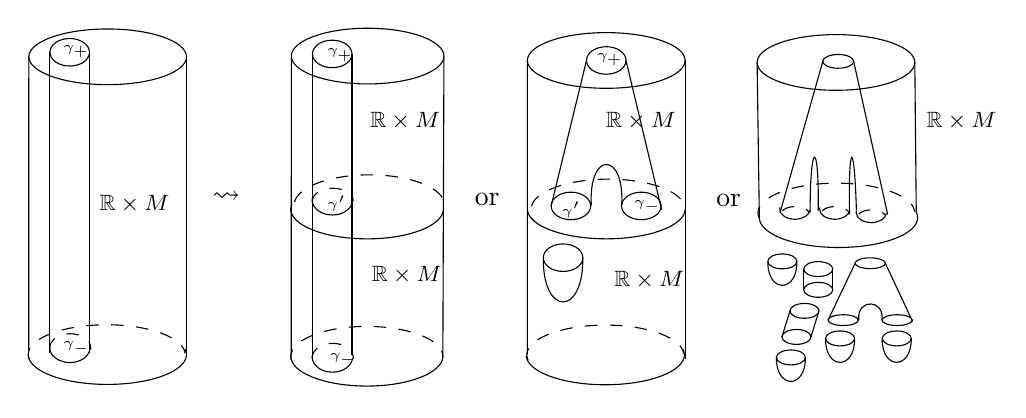
\begin{tikzpicture}[x=0.6pt,y=0.6pt,yscale=-1,xscale=1]
%uncomment if require: \path (0,300); %set diagram left start at 0, and has height of 300

%Shape: Ellipse [id:dp056395190934285244] 
\draw   (30.05,42.21) .. controls (30.05,32.95) and (51.31,25.44) .. (77.54,25.44) .. controls (103.76,25.44) and (125.02,32.95) .. (125.02,42.21) .. controls (125.02,51.48) and (103.76,58.98) .. (77.54,58.98) .. controls (51.31,58.98) and (30.05,51.48) .. (30.05,42.21) -- cycle ;
%Shape: Arc [id:dp6990177911205233] 
\draw  [draw opacity=0] (124.2,218.19) .. controls (124.74,219.28) and (125.02,220.4) .. (125.02,221.54) .. controls (125.02,231.47) and (103.68,239.51) .. (77.36,239.51) .. controls (51.54,239.51) and (30.52,231.77) .. (29.72,222.11) -- (77.36,221.54) -- cycle ; \draw   (124.2,218.19) .. controls (124.74,219.28) and (125.02,220.4) .. (125.02,221.54) .. controls (125.02,231.47) and (103.68,239.51) .. (77.36,239.51) .. controls (51.54,239.51) and (30.52,231.77) .. (29.72,222.11) ;  
%Straight Lines [id:da0017531833743447134] 
\draw    (30.05,41.97) -- (30.01,219.17) ;
%Straight Lines [id:da06191856902561077] 
\draw    (125.02,42.21) -- (125.02,221.93) ;
%Shape: Arc [id:dp7515744636820547] 
\draw  [draw opacity=0][dash pattern={on 4.5pt off 4.5pt}] (30.51,224.86) .. controls (29.98,223.78) and (29.7,222.67) .. (29.7,221.54) .. controls (29.7,211.61) and (50.85,203.57) .. (76.94,203.57) .. controls (102.32,203.57) and (123.02,211.19) .. (124.12,220.74) -- (76.94,221.54) -- cycle ; \draw  [dash pattern={on 4.5pt off 4.5pt}] (30.51,224.86) .. controls (29.98,223.78) and (29.7,222.67) .. (29.7,221.54) .. controls (29.7,211.61) and (50.85,203.57) .. (76.94,203.57) .. controls (102.32,203.57) and (123.02,211.19) .. (124.12,220.74) ;  
%Shape: Ellipse [id:dp170371749578063] 
\draw   (42.78,39.48) .. controls (42.78,34.9) and (48.11,31.19) .. (54.68,31.19) .. controls (61.25,31.19) and (66.58,34.9) .. (66.58,39.48) .. controls (66.58,44.06) and (61.25,47.77) .. (54.68,47.77) .. controls (48.11,47.77) and (42.78,44.06) .. (42.78,39.48) -- cycle ;
%Straight Lines [id:da7961683638948691] 
\draw    (42.78,39.48) -- (42.78,220.58) ;
%Straight Lines [id:da10134655093172151] 
\draw    (66.58,39.48) -- (66.58,220.58) ;
%Shape: Ellipse [id:dp0975147561159333] 
\draw   (188.15,41.77) .. controls (188.15,32.51) and (208.73,25) .. (234.11,25) .. controls (259.48,25) and (280.06,32.51) .. (280.06,41.77) .. controls (280.06,51.04) and (259.48,58.55) .. (234.11,58.55) .. controls (208.73,58.55) and (188.15,51.04) .. (188.15,41.77) -- cycle ;
%Shape: Arc [id:dp3077894307206215] 
\draw  [draw opacity=0] (279.39,222.94) .. controls (278.85,232.68) and (258.56,240.51) .. (233.6,240.51) .. controls (208.31,240.51) and (187.8,232.47) .. (187.8,222.54) .. controls (187.8,221.51) and (188.02,220.51) .. (188.44,219.53) -- (233.6,222.54) -- cycle ; \draw   (279.39,222.94) .. controls (278.85,232.68) and (258.56,240.51) .. (233.6,240.51) .. controls (208.31,240.51) and (187.8,232.47) .. (187.8,222.54) .. controls (187.8,221.51) and (188.02,220.51) .. (188.44,219.53) ;  
%Straight Lines [id:da4345493582140463] 
\draw    (188.15,42.97) -- (188.11,220.17) ;
%Straight Lines [id:da7275152931898132] 
\draw    (280.06,41.77) -- (279.4,223.71) ;
%Shape: Arc [id:dp15000914940586108] 
\draw  [draw opacity=0][dash pattern={on 4.5pt off 4.5pt}] (188.53,225.76) .. controls (188.05,224.72) and (187.8,223.64) .. (187.8,222.54) .. controls (187.8,212.61) and (208.3,204.57) .. (233.6,204.57) .. controls (258.89,204.57) and (279.39,212.61) .. (279.39,222.54) .. controls (279.39,222.67) and (279.39,222.8) .. (279.38,222.92) -- (233.6,222.54) -- cycle ; \draw  [dash pattern={on 4.5pt off 4.5pt}] (188.53,225.76) .. controls (188.05,224.72) and (187.8,223.64) .. (187.8,222.54) .. controls (187.8,212.61) and (208.3,204.57) .. (233.6,204.57) .. controls (258.89,204.57) and (279.39,212.61) .. (279.39,222.54) .. controls (279.39,222.67) and (279.39,222.8) .. (279.38,222.92) ;  
%Shape: Ellipse [id:dp7257031377511021] 
\draw   (200.88,40.48) .. controls (200.88,35.9) and (206.21,32.19) .. (212.78,32.19) .. controls (219.35,32.19) and (224.68,35.9) .. (224.68,40.48) .. controls (224.68,45.06) and (219.35,48.77) .. (212.78,48.77) .. controls (206.21,48.77) and (200.88,45.06) .. (200.88,40.48) -- cycle ;
%Straight Lines [id:da41430031772787657] 
\draw    (200.88,40.48) -- (200.88,221.58) ;
%Straight Lines [id:da8322496496190563] 
\draw    (224.68,40.48) -- (224.68,221.58) ;
%Shape: Arc [id:dp9948607311319655] 
\draw  [draw opacity=0] (279.72,134.27) .. controls (279.18,144.02) and (258.81,151.85) .. (233.76,151.85) .. controls (208.38,151.85) and (187.8,143.81) .. (187.8,133.88) .. controls (187.8,132.85) and (188.02,131.84) .. (188.45,130.86) -- (233.76,133.88) -- cycle ; \draw   (279.72,134.27) .. controls (279.18,144.02) and (258.81,151.85) .. (233.76,151.85) .. controls (208.38,151.85) and (187.8,143.81) .. (187.8,133.88) .. controls (187.8,132.85) and (188.02,131.84) .. (188.45,130.86) ;  
%Shape: Arc [id:dp47440163389587364] 
\draw  [draw opacity=0][dash pattern={on 4.5pt off 4.5pt}] (190.15,129.6) .. controls (192.26,120.45) and (211.6,113.29) .. (235.15,113.29) .. controls (260.12,113.29) and (280.35,121.34) .. (280.35,131.26) .. controls (280.35,132.27) and (280.14,133.26) .. (279.74,134.23) -- (235.15,131.26) -- cycle ; \draw  [dash pattern={on 4.5pt off 4.5pt}] (190.15,129.6) .. controls (192.26,120.45) and (211.6,113.29) .. (235.15,113.29) .. controls (260.12,113.29) and (280.35,121.34) .. (280.35,131.26) .. controls (280.35,132.27) and (280.14,133.26) .. (279.74,134.23) ;  
%Shape: Arc [id:dp6804839012339676] 
\draw  [draw opacity=0] (225.01,223.83) .. controls (224.48,228.48) and (219.25,232.13) .. (212.89,232.13) .. controls (206.17,232.13) and (200.72,228.07) .. (200.72,223.05) .. controls (200.72,222.56) and (200.77,222.07) .. (200.87,221.6) -- (212.89,223.05) -- cycle ; \draw   (225.01,223.83) .. controls (224.48,228.48) and (219.25,232.13) .. (212.89,232.13) .. controls (206.17,232.13) and (200.72,228.07) .. (200.72,223.05) .. controls (200.72,222.56) and (200.77,222.07) .. (200.87,221.6) ;  
%Shape: Arc [id:dp4500398352394417] 
\draw  [draw opacity=0][dash pattern={on 4.5pt off 4.5pt}] (200.83,224.21) .. controls (200.78,223.92) and (200.76,223.62) .. (200.76,223.33) .. controls (200.76,218.61) and (206.29,214.78) .. (213.11,214.78) .. controls (219.93,214.78) and (225.46,218.61) .. (225.46,223.33) .. controls (225.46,223.6) and (225.45,223.88) .. (225.41,224.15) -- (213.11,223.33) -- cycle ; \draw  [dash pattern={on 4.5pt off 4.5pt}] (200.83,224.21) .. controls (200.78,223.92) and (200.76,223.62) .. (200.76,223.33) .. controls (200.76,218.61) and (206.29,214.78) .. (213.11,214.78) .. controls (219.93,214.78) and (225.46,218.61) .. (225.46,223.33) .. controls (225.46,223.6) and (225.45,223.88) .. (225.41,224.15) ;  
%Shape: Arc [id:dp10273519473058612] 
\draw  [draw opacity=0] (224.88,126.86) .. controls (225,127.36) and (225.05,127.88) .. (225.05,128.4) .. controls (225.05,133.42) and (219.61,137.48) .. (212.89,137.48) .. controls (206.17,137.48) and (200.72,133.42) .. (200.72,128.4) .. controls (200.72,127.91) and (200.77,127.42) .. (200.87,126.95) -- (212.89,128.4) -- cycle ; \draw   (224.88,126.86) .. controls (225,127.36) and (225.05,127.88) .. (225.05,128.4) .. controls (225.05,133.42) and (219.61,137.48) .. (212.89,137.48) .. controls (206.17,137.48) and (200.72,133.42) .. (200.72,128.4) .. controls (200.72,127.91) and (200.77,127.42) .. (200.87,126.95) ;  
%Shape: Arc [id:dp9560702304930155] 
\draw  [draw opacity=0][dash pattern={on 4.5pt off 4.5pt}] (200.84,130.15) .. controls (200.79,129.87) and (200.76,129.57) .. (200.76,129.28) .. controls (200.76,124.89) and (206.29,121.33) .. (213.11,121.33) .. controls (219.82,121.33) and (225.28,124.77) .. (225.46,129.06) -- (213.11,129.28) -- cycle ; \draw  [dash pattern={on 4.5pt off 4.5pt}] (200.84,130.15) .. controls (200.79,129.87) and (200.76,129.57) .. (200.76,129.28) .. controls (200.76,124.89) and (206.29,121.33) .. (213.11,121.33) .. controls (219.82,121.33) and (225.28,124.77) .. (225.46,129.06) ;  
%Shape: Arc [id:dp7266228856012471] 
\draw  [draw opacity=0] (66.91,218.04) .. controls (66.38,222.69) and (61.16,226.34) .. (54.79,226.34) .. controls (48.07,226.34) and (42.62,222.27) .. (42.62,217.26) .. controls (42.62,216.76) and (42.67,216.28) .. (42.78,215.81) -- (54.79,217.26) -- cycle ; \draw   (66.91,218.04) .. controls (66.38,222.69) and (61.16,226.34) .. (54.79,226.34) .. controls (48.07,226.34) and (42.62,222.27) .. (42.62,217.26) .. controls (42.62,216.76) and (42.67,216.28) .. (42.78,215.81) ;  
%Shape: Arc [id:dp3689040331833249] 
\draw  [draw opacity=0][dash pattern={on 4.5pt off 4.5pt}] (42.73,218.41) .. controls (42.68,218.12) and (42.66,217.83) .. (42.66,217.53) .. controls (42.66,212.81) and (48.19,208.99) .. (55.01,208.99) .. controls (61.84,208.99) and (67.37,212.81) .. (67.37,217.53) .. controls (67.37,217.81) and (67.35,218.08) .. (67.31,218.35) -- (55.01,217.53) -- cycle ; \draw  [dash pattern={on 4.5pt off 4.5pt}] (42.73,218.41) .. controls (42.68,218.12) and (42.66,217.83) .. (42.66,217.53) .. controls (42.66,212.81) and (48.19,208.99) .. (55.01,208.99) .. controls (61.84,208.99) and (67.37,212.81) .. (67.37,217.53) .. controls (67.37,217.81) and (67.35,218.08) .. (67.31,218.35) ;  
%Shape: Ellipse [id:dp0661139858681199] 
\draw   (330.32,44.41) .. controls (330.32,35.15) and (351.58,27.64) .. (377.81,27.64) .. controls (404.03,27.64) and (425.29,35.15) .. (425.29,44.41) .. controls (425.29,53.67) and (404.03,61.18) .. (377.81,61.18) .. controls (351.58,61.18) and (330.32,53.67) .. (330.32,44.41) -- cycle ;
%Shape: Arc [id:dp8033107315109083] 
\draw  [draw opacity=0] (424.04,218.39) .. controls (424.58,219.47) and (424.87,220.59) .. (424.87,221.74) .. controls (424.87,231.66) and (403.53,239.71) .. (377.21,239.71) .. controls (351.39,239.71) and (330.36,231.97) .. (329.57,222.3) -- (377.21,221.74) -- cycle ; \draw   (424.04,218.39) .. controls (424.58,219.47) and (424.87,220.59) .. (424.87,221.74) .. controls (424.87,231.66) and (403.53,239.71) .. (377.21,239.71) .. controls (351.39,239.71) and (330.36,231.97) .. (329.57,222.3) ;  
%Straight Lines [id:da09066507708598825] 
\draw    (330.32,44.41) -- (330.28,221.6) ;
%Straight Lines [id:da3413965171016031] 
\draw    (425.29,44.41) -- (425.29,224.13) ;
%Shape: Arc [id:dp36547829111768615] 
\draw  [draw opacity=0][dash pattern={on 4.5pt off 4.5pt}] (330.78,225.06) .. controls (330.25,223.98) and (329.97,222.87) .. (329.97,221.74) .. controls (329.97,211.81) and (351.12,203.77) .. (377.21,203.77) .. controls (402.59,203.77) and (423.3,211.38) .. (424.39,220.94) -- (377.21,221.74) -- cycle ; \draw  [dash pattern={on 4.5pt off 4.5pt}] (330.78,225.06) .. controls (330.25,223.98) and (329.97,222.87) .. (329.97,221.74) .. controls (329.97,211.81) and (351.12,203.77) .. (377.21,203.77) .. controls (402.59,203.77) and (423.3,211.38) .. (424.39,220.94) ;  
%Shape: Ellipse [id:dp8629704518272938] 
\draw   (365.91,44.41) .. controls (365.91,39.83) and (371.24,36.12) .. (377.81,36.12) .. controls (384.38,36.12) and (389.71,39.83) .. (389.71,44.41) .. controls (389.71,48.99) and (384.38,52.7) .. (377.81,52.7) .. controls (371.24,52.7) and (365.91,48.99) .. (365.91,44.41) -- cycle ;
%Straight Lines [id:da8452678956957251] 
\draw    (365.91,44.41) -- (344.63,132.03) ;
%Straight Lines [id:da19999367359767395] 
\draw    (389.71,44.41) -- (411.17,134.3) ;
%Curve Lines [id:da16572232996503655] 
\draw    (368.81,131.66) .. controls (366.95,98.15) and (389.34,99.35) .. (387.05,132.03) ;
%Shape: Arc [id:dp6457528380286801] 
\draw  [draw opacity=0] (425.29,134.26) .. controls (424.72,144) and (403.68,151.83) .. (377.8,151.83) .. controls (351.71,151.83) and (330.53,143.87) .. (330.3,134.01) -- (377.8,133.85) -- cycle ; \draw   (425.29,134.26) .. controls (424.72,144) and (403.68,151.83) .. (377.8,151.83) .. controls (351.71,151.83) and (330.53,143.87) .. (330.3,134.01) ;  
%Shape: Arc [id:dp19216152259248287] 
\draw  [draw opacity=0][dash pattern={on 4.5pt off 4.5pt}] (332.81,132.15) .. controls (335.03,123.02) and (354.84,115.88) .. (378.95,115.88) .. controls (403.7,115.88) and (423.92,123.41) .. (425.23,132.88) -- (378.95,133.85) -- cycle ; \draw  [dash pattern={on 4.5pt off 4.5pt}] (332.81,132.15) .. controls (335.03,123.02) and (354.84,115.88) .. (378.95,115.88) .. controls (403.7,115.88) and (423.92,123.41) .. (425.23,132.88) ;  
%Shape: Ellipse [id:dp16448002790374439] 
\draw   (344.63,132.03) .. controls (344.63,127.45) and (349.95,123.74) .. (356.53,123.74) .. controls (363.1,123.74) and (368.43,127.45) .. (368.43,132.03) .. controls (368.43,136.61) and (363.1,140.32) .. (356.53,140.32) .. controls (349.95,140.32) and (344.63,136.61) .. (344.63,132.03) -- cycle ;
%Shape: Ellipse [id:dp9809662464110647] 
\draw   (387.05,132.03) .. controls (387.05,127.45) and (392.37,123.74) .. (398.94,123.74) .. controls (405.52,123.74) and (410.84,127.45) .. (410.84,132.03) .. controls (410.84,136.61) and (405.52,140.32) .. (398.94,140.32) .. controls (392.37,140.32) and (387.05,136.61) .. (387.05,132.03) -- cycle ;
%Shape: Ellipse [id:dp08366558813265468] 
\draw   (339.91,163.18) .. controls (339.91,158.6) and (345.24,154.89) .. (351.81,154.89) .. controls (358.39,154.89) and (363.71,158.6) .. (363.71,163.18) .. controls (363.71,167.76) and (358.39,171.47) .. (351.81,171.47) .. controls (345.24,171.47) and (339.91,167.76) .. (339.91,163.18) -- cycle ;
%Curve Lines [id:da09367632050515562] 
\draw    (339.91,163.18) .. controls (339.4,198.73) and (364.14,198.73) .. (363.71,163.18) ;
%Shape: Ellipse [id:dp8188508828087644] 
\draw   (468.66,45.61) .. controls (468.66,36.34) and (489.92,28.83) .. (516.14,28.83) .. controls (542.37,28.83) and (563.63,36.34) .. (563.63,45.61) .. controls (563.63,54.87) and (542.37,62.38) .. (516.14,62.38) .. controls (489.92,62.38) and (468.66,54.87) .. (468.66,45.61) -- cycle ;
%Shape: Arc [id:dp8117575286418532] 
\draw  [draw opacity=0] (564.51,135.73) .. controls (565.05,136.81) and (565.33,137.93) .. (565.33,139.08) .. controls (565.33,149) and (543.99,157.05) .. (517.67,157.05) .. controls (491.85,157.05) and (470.83,149.31) .. (470.04,139.64) -- (517.67,139.08) -- cycle ; \draw   (564.51,135.73) .. controls (565.05,136.81) and (565.33,137.93) .. (565.33,139.08) .. controls (565.33,149) and (543.99,157.05) .. (517.67,157.05) .. controls (491.85,157.05) and (470.83,149.31) .. (470.04,139.64) ;  
%Straight Lines [id:da331799661099899] 
\draw    (468.66,45.37) -- (470.01,139.6) ;
%Straight Lines [id:da9563297554519652] 
\draw    (563.63,45.61) -- (564.51,135.73) ;
%Shape: Arc [id:dp08014198609210887] 
\draw  [draw opacity=0][dash pattern={on 4.5pt off 4.5pt}] (470.01,139.6) .. controls (469.48,138.52) and (469.21,137.41) .. (469.21,136.28) .. controls (469.21,126.35) and (490.35,118.31) .. (516.44,118.31) .. controls (541.82,118.31) and (562.53,125.92) .. (563.63,135.48) -- (516.44,136.28) -- cycle ; \draw  [dash pattern={on 4.5pt off 4.5pt}] (470.01,139.6) .. controls (469.48,138.52) and (469.21,137.41) .. (469.21,136.28) .. controls (469.21,126.35) and (490.35,118.31) .. (516.44,118.31) .. controls (541.82,118.31) and (562.53,125.92) .. (563.63,135.48) ;  
%Shape: Ellipse [id:dp11318015897818423] 
\draw   (508.22,44.95) .. controls (508.22,42.66) and (512.38,40.81) .. (517.51,40.81) .. controls (522.64,40.81) and (526.8,42.66) .. (526.8,44.95) .. controls (526.8,47.24) and (522.64,49.09) .. (517.51,49.09) .. controls (512.38,49.09) and (508.22,47.24) .. (508.22,44.95) -- cycle ;
%Shape: Arc [id:dp5481702992712509] 
\draw  [draw opacity=0] (546.51,136.57) .. controls (546.06,139.65) and (542.17,142.05) .. (537.43,142.05) .. controls (532.39,142.05) and (528.31,139.34) .. (528.31,135.99) .. controls (528.31,135.62) and (528.36,135.25) .. (528.46,134.9) -- (537.43,135.99) -- cycle ; \draw   (546.51,136.57) .. controls (546.06,139.65) and (542.17,142.05) .. (537.43,142.05) .. controls (532.39,142.05) and (528.31,139.34) .. (528.31,135.99) .. controls (528.31,135.62) and (528.36,135.25) .. (528.46,134.9) ;  
%Shape: Arc [id:dp03984534439684717] 
\draw  [draw opacity=0][dash pattern={on 4.5pt off 4.5pt}] (529.88,136.9) .. controls (531.49,135.39) and (534.33,134.38) .. (537.57,134.38) .. controls (541.2,134.38) and (544.33,135.64) .. (545.79,137.47) -- (537.57,139.78) -- cycle ; \draw  [dash pattern={on 4.5pt off 4.5pt}] (529.88,136.9) .. controls (531.49,135.39) and (534.33,134.38) .. (537.57,134.38) .. controls (541.2,134.38) and (544.33,135.64) .. (545.79,137.47) ;  
%Straight Lines [id:da3617949510353735] 
\draw    (508.22,44.95) -- (482.46,136.1) ;
%Straight Lines [id:da649340590604436] 
\draw    (526.8,44.95) -- (547.3,137.17) ;
%Curve Lines [id:da8727790296078328] 
\draw    (500.59,136) .. controls (500.55,91.73) and (506.07,91.73) .. (505.46,134.9) ;
%Curve Lines [id:da4875409262510293] 
\draw    (524.3,137.17) .. controls (523.55,91.73) and (527.23,91.73) .. (528.46,134.9) ;
%Shape: Ellipse [id:dp7111828464384535] 
\draw   (475.13,165.41) .. controls (475.13,162.93) and (479.04,160.93) .. (483.87,160.93) .. controls (488.7,160.93) and (492.61,162.93) .. (492.61,165.41) .. controls (492.61,167.89) and (488.7,169.89) .. (483.87,169.89) .. controls (479.04,169.89) and (475.13,167.89) .. (475.13,165.41) -- cycle ;
%Curve Lines [id:da9672709945361355] 
\draw    (475.13,165.41) .. controls (474.75,184.63) and (492.92,184.63) .. (492.61,165.41) ;
%Shape: Ellipse [id:dp8770495266103071] 
\draw   (496.76,170.05) .. controls (496.76,167.57) and (500.67,165.56) .. (505.5,165.56) .. controls (510.33,165.56) and (514.24,167.57) .. (514.24,170.05) .. controls (514.24,172.52) and (510.33,174.53) .. (505.5,174.53) .. controls (500.67,174.53) and (496.76,172.52) .. (496.76,170.05) -- cycle ;
%Shape: Ellipse [id:dp4700005658957731] 
\draw   (496.76,182.56) .. controls (496.76,180.08) and (500.67,178.07) .. (505.5,178.07) .. controls (510.33,178.07) and (514.24,180.08) .. (514.24,182.56) .. controls (514.24,185.03) and (510.33,187.04) .. (505.5,187.04) .. controls (500.67,187.04) and (496.76,185.03) .. (496.76,182.56) -- cycle ;
%Shape: Ellipse [id:dp3742015758632733] 
\draw   (488.45,195.21) .. controls (488.45,192.74) and (492.36,190.73) .. (497.19,190.73) .. controls (502.01,190.73) and (505.93,192.74) .. (505.93,195.21) .. controls (505.93,197.69) and (502.01,199.69) .. (497.19,199.69) .. controls (492.36,199.69) and (488.45,197.69) .. (488.45,195.21) -- cycle ;
%Shape: Ellipse [id:dp05712935955362908] 
\draw   (483.6,210.9) .. controls (483.6,208.43) and (487.51,206.42) .. (492.34,206.42) .. controls (497.16,206.42) and (501.08,208.43) .. (501.08,210.9) .. controls (501.08,213.38) and (497.16,215.39) .. (492.34,215.39) .. controls (487.51,215.39) and (483.6,213.38) .. (483.6,210.9) -- cycle ;
%Straight Lines [id:da2384391731418305] 
\draw    (496.76,170.05) -- (496.76,182.56) ;
%Straight Lines [id:da33392656495348927] 
\draw    (514.24,170.05) -- (514.24,182.56) ;
%Straight Lines [id:da566045394847106] 
\draw    (505.93,195.21) -- (501.08,210.9) ;
%Straight Lines [id:da5614446278591068] 
\draw    (488.45,195.21) -- (483.6,210.9) ;
%Shape: Ellipse [id:dp035227786182282506] 
\draw   (480.27,223.26) .. controls (480.27,220.78) and (484.18,218.77) .. (489.01,218.77) .. controls (493.84,218.77) and (497.75,220.78) .. (497.75,223.26) .. controls (497.75,225.73) and (493.84,227.74) .. (489.01,227.74) .. controls (484.18,227.74) and (480.27,225.73) .. (480.27,223.26) -- cycle ;
%Curve Lines [id:da7379429542962657] 
\draw    (480.27,223.26) .. controls (479.89,242.47) and (498.06,242.47) .. (497.75,223.26) ;
%Shape: Ellipse [id:dp5542296065150325] 
\draw   (509.9,211.8) .. controls (509.9,209.33) and (513.82,207.32) .. (518.64,207.32) .. controls (523.47,207.32) and (527.38,209.33) .. (527.38,211.8) .. controls (527.38,214.28) and (523.47,216.29) .. (518.64,216.29) .. controls (513.82,216.29) and (509.9,214.28) .. (509.9,211.8) -- cycle ;
%Curve Lines [id:da7423459609744811] 
\draw    (509.9,211.8) .. controls (509.53,231.02) and (527.7,231.02) .. (527.38,211.8) ;
%Shape: Ellipse [id:dp24342029029087775] 
\draw   (544,211.8) .. controls (544,209.33) and (547.91,207.32) .. (552.74,207.32) .. controls (557.56,207.32) and (561.48,209.33) .. (561.48,211.8) .. controls (561.48,214.28) and (557.56,216.29) .. (552.74,216.29) .. controls (547.91,216.29) and (544,214.28) .. (544,211.8) -- cycle ;
%Curve Lines [id:da21595115366288664] 
\draw    (544,211.8) .. controls (543.62,231.02) and (561.79,231.02) .. (561.48,211.8) ;
%Shape: Ellipse [id:dp9507589820584572] 
\draw   (527.68,166.53) .. controls (527.68,164.74) and (531.76,163.28) .. (536.79,163.28) .. controls (541.82,163.28) and (545.9,164.74) .. (545.9,166.53) .. controls (545.9,168.32) and (541.82,169.77) .. (536.79,169.77) .. controls (531.76,169.77) and (527.68,168.32) .. (527.68,166.53) -- cycle ;
%Straight Lines [id:da7901347005685313] 
\draw    (527.68,166.53) -- (511.39,200.8) ;
%Straight Lines [id:da056288864133154926] 
\draw    (545.9,166.53) -- (562.33,201.69) ;
%Curve Lines [id:da988145377883118] 
\draw    (529.9,200.65) .. controls (528.48,187.55) and (545.61,188.02) .. (543.86,200.8) ;
%Shape: Ellipse [id:dp23604569535188302] 
\draw   (511.39,200.8) .. controls (511.39,199.01) and (515.47,197.55) .. (520.5,197.55) .. controls (525.53,197.55) and (529.61,199.01) .. (529.61,200.8) .. controls (529.61,202.59) and (525.53,204.04) .. (520.5,204.04) .. controls (515.47,204.04) and (511.39,202.59) .. (511.39,200.8) -- cycle ;
%Shape: Ellipse [id:dp7261778653447537] 
\draw   (543.86,200.8) .. controls (543.86,199.01) and (547.94,197.55) .. (552.97,197.55) .. controls (558,197.55) and (562.08,199.01) .. (562.08,200.8) .. controls (562.08,202.59) and (558,204.04) .. (552.97,204.04) .. controls (547.94,204.04) and (543.86,202.59) .. (543.86,200.8) -- cycle ;
%Shape: Arc [id:dp3746223374313047] 
\draw  [draw opacity=0] (524.51,134.57) .. controls (524.06,137.65) and (520.17,140.05) .. (515.43,140.05) .. controls (510.39,140.05) and (506.31,137.34) .. (506.31,133.99) .. controls (506.31,133.62) and (506.36,133.25) .. (506.46,132.9) -- (515.43,133.99) -- cycle ; \draw   (524.51,134.57) .. controls (524.06,137.65) and (520.17,140.05) .. (515.43,140.05) .. controls (510.39,140.05) and (506.31,137.34) .. (506.31,133.99) .. controls (506.31,133.62) and (506.36,133.25) .. (506.46,132.9) ;  
%Shape: Arc [id:dp21450518339030733] 
\draw  [draw opacity=0][dash pattern={on 4.5pt off 4.5pt}] (507.88,134.9) .. controls (509.49,133.39) and (512.33,132.38) .. (515.57,132.38) .. controls (519.2,132.38) and (522.33,133.64) .. (523.79,135.47) -- (515.57,137.78) -- cycle ; \draw  [dash pattern={on 4.5pt off 4.5pt}] (507.88,134.9) .. controls (509.49,133.39) and (512.33,132.38) .. (515.57,132.38) .. controls (519.2,132.38) and (522.33,133.64) .. (523.79,135.47) ;  
%Shape: Arc [id:dp37481817018727304] 
\draw  [draw opacity=0] (500.51,134.57) .. controls (500.06,137.65) and (496.17,140.05) .. (491.43,140.05) .. controls (486.39,140.05) and (482.31,137.34) .. (482.31,133.99) .. controls (482.31,133.62) and (482.36,133.25) .. (482.46,132.9) -- (491.43,133.99) -- cycle ; \draw   (500.51,134.57) .. controls (500.06,137.65) and (496.17,140.05) .. (491.43,140.05) .. controls (486.39,140.05) and (482.31,137.34) .. (482.31,133.99) .. controls (482.31,133.62) and (482.36,133.25) .. (482.46,132.9) ;  
%Shape: Arc [id:dp03724951552805966] 
\draw  [draw opacity=0][dash pattern={on 4.5pt off 4.5pt}] (483.88,134.9) .. controls (485.49,133.39) and (488.33,132.38) .. (491.57,132.38) .. controls (495.2,132.38) and (498.33,133.64) .. (499.79,135.47) -- (491.57,137.78) -- cycle ; \draw  [dash pattern={on 4.5pt off 4.5pt}] (483.88,134.9) .. controls (485.49,133.39) and (488.33,132.38) .. (491.57,132.38) .. controls (495.2,132.38) and (498.33,133.64) .. (499.79,135.47) ;  

% Text Node
\draw (139.08,121.83) node [anchor=north west][inner sep=0.75pt]    {$\rightsquigarrow $};
% Text Node
\draw (71.12,123.83) node [anchor=north west][inner sep=0.75pt]  [font=\footnotesize]  {$\mathbb{R} \times M$};
% Text Node
\draw (208.07,35.68) node [anchor=north west][inner sep=0.75pt]  [font=\tiny]  {$\gamma _{+}$};
% Text Node
\draw (49.15,212.24) node [anchor=north west][inner sep=0.75pt]  [font=\tiny]  {$\gamma _{-}$};
% Text Node
\draw (209.61,219.23) node [anchor=north west][inner sep=0.75pt]  [font=\tiny]  {$\gamma _{-}$};
% Text Node
\draw (208.07,124.24) node [anchor=north west][inner sep=0.75pt]  [font=\tiny]  {$\gamma '$};
% Text Node
\draw (297.07,122.73) node [anchor=north west][inner sep=0.75pt]   [align=left] {or};
% Text Node
\draw (49.15,33.72) node [anchor=north west][inner sep=0.75pt]  [font=\tiny]  {$\gamma _{+}$};
% Text Node
\draw (392.94,127.04) node [anchor=north west][inner sep=0.75pt]  [font=\tiny]  {$\gamma _{-}$};
% Text Node
\draw (349.35,128.14) node [anchor=north west][inner sep=0.75pt]  [font=\tiny]  {$\gamma '$};
% Text Node
\draw (370.56,38.38) node [anchor=north west][inner sep=0.75pt]  [font=\tiny]  {$\gamma _{+}$};
% Text Node
\draw (442.53,123.33) node [anchor=north west][inner sep=0.75pt]   [align=left] {or};
% Text Node
\draw (235.12,166.83) node [anchor=north west][inner sep=0.75pt]  [font=\footnotesize]  {$\mathbb{R} \times M$};
% Text Node
\draw (234.12,73.83) node [anchor=north west][inner sep=0.75pt]  [font=\footnotesize]  {$\mathbb{R} \times M$};
% Text Node
\draw (376.12,73.83) node [anchor=north west][inner sep=0.75pt]  [font=\footnotesize]  {$\mathbb{R} \times M$};
% Text Node
\draw (381.12,169.83) node [anchor=north west][inner sep=0.75pt]  [font=\footnotesize]  {$\mathbb{R} \times M$};
% Text Node
\draw (569.12,73.83) node [anchor=north west][inner sep=0.75pt]  [font=\footnotesize]  {$\mathbb{R} \times M$};


\end{tikzpicture}

\end{center}

where for the rightmost diagram, each of the bottom components is a map to $\mathbb{R}^n$.

\begin{definition}

Let $(F,j)$ be a Riemann surface, $\dot{F}=F$ a finite subset, and $u:(\dot{F},j)\stackrel{J-\text{holomorphic}}{\to} (\mathbb{R}\times M, J)$. Then the \textbf{Hofer energy} is
\[
E(u)=\sup_{\phi \in \mathcal{C}} \int_{\dot{F}} u^* d(\phi, \alpha)
\]
where
\[
\mathcal{C} = \left\{ \phi: \mathbb{R} \to [1,2] \mid
\begin{cases}
\phi(s) = 1 & \text{if } s \ll 0, \\
\phi(s) = 2 & \text{if } s \gg 0, \\
\phi'(s) \ge 0 & \text{for all } s \in \mathbb{R}
\end{cases}
\right\}
\]

\end{definition}

\begin{proposition}

\begin{align*}
E(u)&= 2\sum_{i=1}^{k_+} \mathcal{A}(\gamma_{+,i})-\sum_{i=1}^{k_-} \mathcal{A}(\gamma_{-,i}) \\
&\ge 0.
\end{align*}

\end{proposition}

\section{Grading}

\begin{theorem}

If $u: (\dot{E}, j)\to \mathbb{R}\times M$ is $J$-holomorphic, the following are equivalent:
\begin{itemize}
\item $E(u)<\infty$
\item For any puncture $p$ of $\dot{F}$, either $p$ is removable or $u$ converges to some Reeb orbit along $P$.
\end{itemize}

\end{theorem}

Assume the $H_1(M; \mathbb{Z})$ is torsion free. If $H_1(M)=0$, then for each Reeb orbit $\gamma$, fix a surface $F_\gamma \subset M$ spanning $\gamma$. If $H_1(M; \mathbb{Z})\neq 0$, choose a basis of $H_1(M)$ and represent it by oriented curves $c_1,...c_k$. Choose a trivialization of $\xi/c_1$. For any Reeb orbit $\gamma$, choose $F_\gamma$ such that $[\partial F_\gamma]=[\gamma]-\sum n_i [c_i]$. Choose a trivialization of $\xi \mid_{\gamma}$ so that it extends over $F_\gamma$ and agrees with the trivialization of $\xi/c_i$. This defines a Conley-Zehder index for each $\gamma$.

For each $J$-holomorphic cylinder $u$, we can attach $F_{\gamma_+}$ and $F_{\gamma_-}$:
\begin{center}
\tikzset{every picture/.style={line width=0.75pt}} %set default line width to 0.75pt        

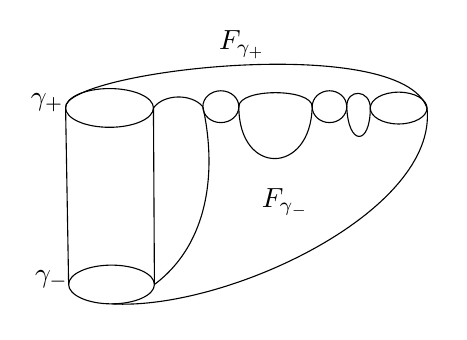
\begin{tikzpicture}[x=0.5pt,y=0.5pt,yscale=-1,xscale=1]
%uncomment if require: \path (0,300); %set diagram left start at 0, and has height of 300

%Shape: Ellipse [id:dp8909013950100437] 
\draw   (85,82) .. controls (85,74.27) and (99.21,68) .. (116.75,68) .. controls (134.29,68) and (148.5,74.27) .. (148.5,82) .. controls (148.5,89.73) and (134.29,96) .. (116.75,96) .. controls (99.21,96) and (85,89.73) .. (85,82) -- cycle ;
%Straight Lines [id:da939999364801372] 
\draw    (85,82) -- (87.2,209.6) ;
%Straight Lines [id:da32030547024849] 
\draw    (148.5,82) -- (149.2,209.6) ;
%Shape: Ellipse [id:dp22593738557210807] 
\draw   (87.2,209.6) .. controls (87.2,201.87) and (101.08,195.6) .. (118.2,195.6) .. controls (135.32,195.6) and (149.2,201.87) .. (149.2,209.6) .. controls (149.2,217.33) and (135.32,223.6) .. (118.2,223.6) .. controls (101.08,223.6) and (87.2,217.33) .. (87.2,209.6) -- cycle ;
%Shape: Ellipse [id:dp3903650035201627] 
\draw   (184.2,81.1) .. controls (184.2,74.75) and (190.02,69.6) .. (197.2,69.6) .. controls (204.38,69.6) and (210.2,74.75) .. (210.2,81.1) .. controls (210.2,87.45) and (204.38,92.6) .. (197.2,92.6) .. controls (190.02,92.6) and (184.2,87.45) .. (184.2,81.1) -- cycle ;
%Shape: Ellipse [id:dp439043297167095] 
\draw   (263.2,81.1) .. controls (263.2,74.75) and (268.8,69.6) .. (275.7,69.6) .. controls (282.6,69.6) and (288.2,74.75) .. (288.2,81.1) .. controls (288.2,87.45) and (282.6,92.6) .. (275.7,92.6) .. controls (268.8,92.6) and (263.2,87.45) .. (263.2,81.1) -- cycle ;
%Shape: Ellipse [id:dp5515211986371753] 
\draw   (305.2,82.1) .. controls (305.2,75.75) and (314.38,70.6) .. (325.7,70.6) .. controls (337.02,70.6) and (346.2,75.75) .. (346.2,82.1) .. controls (346.2,88.45) and (337.02,93.6) .. (325.7,93.6) .. controls (314.38,93.6) and (305.2,88.45) .. (305.2,82.1) -- cycle ;
%Curve Lines [id:da43171084391564163] 
\draw    (118.2,223.6) .. controls (201.2,228.6) and (354.2,156.6) .. (346.2,82.1) ;
%Curve Lines [id:da12535479193092525] 
\draw    (85,82) .. controls (82.2,55.6) and (327.2,26.6) .. (346.2,82.1) ;
%Curve Lines [id:da515259067066461] 
\draw    (288.2,81.1) .. controls (289.2,109.6) and (305.2,109.6) .. (305.2,82.1) ;
%Curve Lines [id:da3208943864453322] 
\draw    (210.2,81.1) .. controls (210.2,131.6) and (262.2,130.6) .. (263.2,81.1) ;
%Curve Lines [id:da7762191468457265] 
\draw    (210.2,81.1) .. controls (210.2,67.6) and (263.2,67.6) .. (263.2,81.1) ;
%Curve Lines [id:da23187615015116236] 
\draw    (288.2,81.1) .. controls (288.2,67.6) and (305.2,68.6) .. (305.2,82.1) ;
%Curve Lines [id:da3836381595978182] 
\draw    (148.5,82) .. controls (156.2,71.6) and (176.2,71.6) .. (184.2,81.1) ;
%Curve Lines [id:da3396096780840039] 
\draw    (149.2,209.6) .. controls (189.2,179.6) and (194.2,126.6) .. (184.2,81.1) ;

% Text Node
\draw (58,69.4) node [anchor=north west][inner sep=0.75pt]    {$\gamma _{+}$};
% Text Node
\draw (61,197.4) node [anchor=north west][inner sep=0.75pt]    {$\gamma _{-}$};
% Text Node
\draw (194,24.4) node [anchor=north west][inner sep=0.75pt]    {$F_{\gamma _{+}}$};
% Text Node
\draw (225,138.4) node [anchor=north west][inner sep=0.75pt]    {$F_{\gamma _{-}}$};

\end{tikzpicture}
\end{center}

which gives an element in $H_2(M)$.

Assume does not exist a contractible Reeb orbits. We define a chain complex $(C_*, \partial)$ where $C_*$ is a free $\mathbb{Q}[H_2(M)]$ module generated by all good Reeb orbits. For each $A\in H_2(M)$, $| A|  = -2 \langle c_1(\xi), A \rangle$, define $\partial_{\gamma_+}= \sum_{\gamma_-, A}\# \mathcal{M}(\gamma_+, \gamma_-, A) e^A \frac{1}{m(\gamma_-)}\gamma_-$ where $m(\gamma_-)$ is the multiplcity of $\gamma_-$. This gives $|\gamma_+| -| \gamma_- | -| A| =1$. Define $| \gamma| =\mu_{c_2}(\gamma)+n-3$.

\begin{definition}

$\gamma$ is \textbf{bad} if $\gamma$ is multiple cover of embedded $\gamma'$ and $\mu_{\text{cz}}(\gamma)-\mu_{\text{cz}}(\gamma')$ is odd.

\end{definition}

\begin{example}

For $\dim \mathcal{M}=3$, $\gamma$ is bad if and only if $\gamma$ is an even multiple cover of a negative hyperbolic one.

\end{example}

If there exists a contractible Reeb orbits:
\vspace{-20pt}
\begin{figure}[htbp]
  \centering
  \includegraphics[width=1\textwidth]{images/bao1.png}
  \label{fig:bi14}
\end{figure}
\vspace{-40pt} % Adjust this value to control the space

This gives the contact homology. One important variant of the contact homology is the (rational) symplectic field theory.

\begin{example}

In $\dim =3$, if $\gamma$ is hyperbolic, then
\[
\mu_{\text{cz}}(\gamma, k) = k \mu_{\text{cz}}(\gamma).
\]

Let $u$ be $J$-holomorphic. If $\text{ind }u = \mu(\gamma_+)-\mu(\gamma)-| A| $. If $u$ is $k$-fold cover of $u'$ and there are no elliptic orbits, then $\text{ind }u = k\cdot \text{ind }u'$.

If $u'$ transverses $\text{ind}$ and $\text{ind } u' \ge 1$, then $\text{ind }u \ge k$. In the definition of $\partial, \text{ind }(u)=1 \implies k=1$.

We can always eliminate elliptic orbits up to any action:
\begin{center}
    
\tikzset{every picture/.style={line width=0.75pt}} %set default line width to 0.75pt        

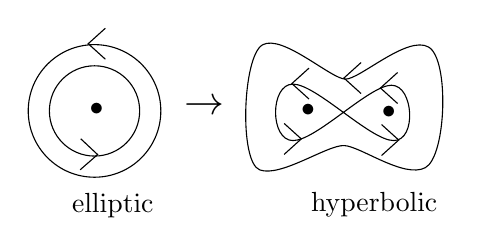
\begin{tikzpicture}[x=0.4pt,y=0.4pt,yscale=-1,xscale=1]
%uncomment if require: \path (0,300); %set diagram left start at 0, and has height of 300

%Shape: Circle [id:dp08144944578189617] 
\draw   (70.82,119.71) .. controls (70.82,86.63) and (97.63,59.82) .. (130.71,59.82) .. controls (163.79,59.82) and (190.6,86.63) .. (190.6,119.71) .. controls (190.6,152.79) and (163.79,179.6) .. (130.71,179.6) .. controls (97.63,179.6) and (70.82,152.79) .. (70.82,119.71) -- cycle ;
%Shape: Circle [id:dp39773554712775216] 
\draw   (89.93,119.71) .. controls (89.93,97.19) and (108.19,78.93) .. (130.71,78.93) .. controls (153.23,78.93) and (171.49,97.19) .. (171.49,119.71) .. controls (171.49,142.23) and (153.23,160.49) .. (130.71,160.49) .. controls (108.19,160.49) and (89.93,142.23) .. (89.93,119.71) -- cycle ;
%Shape: Polygon Curved [id:ds02793189593737866] 
\draw   (399,96.5) .. controls (419,96.5) and (422,146.5) .. (401,146.5) .. controls (380,146.5) and (331,95.5) .. (310,95.5) .. controls (289,95.5) and (289,146.5) .. (310,146.5) .. controls (331,146.5) and (379,96.5) .. (399,96.5) -- cycle ;
%Shape: Polygon Curved [id:ds03073014229495996] 
\draw   (357.5,91) .. controls (370.5,91) and (413.5,51) .. (432.5,62) .. controls (451.5,73) and (448.5,161) .. (429.5,171) .. controls (410.5,181) and (371.5,152) .. (356.5,151) .. controls (341.5,150) and (299,180) .. (280,173) .. controls (261,166) and (264.5,70) .. (282.5,60) .. controls (300.5,50) and (344.5,91) .. (357.5,91) -- cycle ;
\draw   (371.5,104) -- (356,90) -- (371.5,76) ;
\draw   (324.5,109) -- (309,95) -- (324.5,81) ;
\draw   (390,132) -- (405.5,146) -- (390,160) ;
\draw   (302,131) -- (317.5,145) -- (302,159) ;
\draw   (404.5,113) -- (389,99) -- (404.5,85) ;
\draw   (140.5,73) -- (125,59) -- (140.5,45) ;
\draw   (118.25,144.87) -- (133.5,159.14) -- (117.76,172.86) ;

% Text Node
\draw (124,110.4) node [anchor=north west][inner sep=0.75pt]    {$\bullet $};
% Text Node
\draw (315,111.4) node [anchor=north west][inner sep=0.75pt]    {$\bullet $};
% Text Node
\draw (388,113.4) node [anchor=north west][inner sep=0.75pt]    {$\bullet $};
% Text Node
\draw (210,107.4) node [anchor=north west][inner sep=0.75pt]  [font=\Large]  {$\rightarrow $};
% Text Node
\draw (108,192) node [anchor=north west][inner sep=0.75pt]   [align=left] {elliptic};
% Text Node
\draw (324,191) node [anchor=north west][inner sep=0.75pt]   [align=left] {hyperbolic};

\end{tikzpicture}

\end{center}

These two images have the same contact structure, but different contact forms.

\end{example}
\chapter{Semi-Global Kuranishi Structure and Full Contact Homology}
\label{b3}
\abstract{In this lecture, we introduce the semi-global Kuranishi structure. We explore its application in relation to obstruction bundle gluing, including computations of simple examples. The discussion will culminate in the rigorous definition of full contact homology, facilitated by the semi-global Kuranishi structure.}

\section{Introduction}
Suppose $(W,\,d\alpha)$ is an exact symplectic manifold with $\partial W=W_+ + W_-, \alpha|_{W_\pm}=W_{\pm}$, and $J$ an almost complex surface on $\hat{W}$. To count $\text{ind}=0$ $J$-holomorphic cylinders, we obtain a chain map
\[
\Phi: c_*(W_+, \alpha_+, J_+) \to c_*(w_-, \alpha_-, J_-)
\]

Given a 1-parameter family of this data $(W^2, \,d\alpha^2, J^2)$ we want $ \Phi_0 < \Phi_1$ to induce the same map on homology:
\[
\mathcal{M}(\gamma_+, \gamma_-) = \bigsqcup_\iota \{ \iota \}\times \mathcal{M}_{J^2}^{\text{ind}=0} (\gamma_+, \gamma_-).
\]

We want to show that there exists a linear map $K: c_+(W_+, \alpha_+, J_+) \to c_*(W_-, \alpha_-, J_-)$ such that $\Phi_0-\Phi_1 = K\partial + \partial K$.

We have:
\newpage
\vspace{-20pt}
\begin{center}
    \begin{figure}[htbp]
  \centering
  \includegraphics[width=1\textwidth]{images/bao2.png}
  \label{fig:bi14}
\end{figure}
\end{center}
\vspace{-50pt}
For the right most cylinder, we can attach $\mathcal{U}$ to the top half and $\mathcal{M}$ to the bottom half.

For each $\mathcal{U}$, we have a map $\mathcal{S}^{-1}: \mathcal{O}\to [R,\infty)\times M$ and a vector space attached to $\mathcal{O}$ defined by $\ker D_u^*/\mathbb{R} \langle Y \rangle$ where $Y$ comes from variation of $J^2$ and $\mathcal{S}^{-1}(0)$ is the set of curves in $M$ that glue with $\mathcal{U}$.

\section{Semi-Global Kuranishi Structure}

We start with Morse homology case. Let $X$ be a closed manifold, $f: X\to \mathbb{R}$ be a Morse function, $g$ a Riemannian metric, $\phi^t$ the time-$t$ flow of $-\text{grad}_f$, $p\in \text{Crit}(f)$, $\mathcal{D}_p$ be the descending manifold of $p$, and $\mathcal{A}_p$ be the ascending manifold of $p$.

For any $p, q \in \text{Crit}(f)$, 
\[\mathcal{M}(p,q)= \left( \mathcal{A}+q \cap \mathcal{D}_p \right)/\mathbb{R}.
\]

\begin{definition}

An \textbf{interior semi-global Kuranishi chart} is a quadruple $(K, \pi_v: E\to V, \mathcal{L}:V\to E, \psi)$ where
\begin{enumerate}
\item $K\subset M$ is a capacity.
\item $\pi_V: E\to V$ is a finite rank vector bundle of a finite dimensional manifold.
\item $\mathcal{L}$ is a section.
\item $\psi: \mathcal{L}^{-1}(0) \to M$ is homeomorphic onto an open sbuset of $M$ containing $K$.
\item $\dim V - \text{rank} E =\text{vir} \dim\mathcal{M}$
\end{enumerate}

\end{definition}

We order the moduli space $\mathcal{M}_1, \mathcal{M}_2,...$ such that the energy increase. Let
\[
\mathcal{M}_i=\mathcal{M}(p_i, q_i), \qquad E(\mathcal{M}_i)=f(p_i)-f(q_i).
\]
and suppose we have an index tuple $I=(i_1,...,i_n)$ such that $p_{i_m}=q_{i_{m+1}}$. Suppose $S\subset I$ is a subindex tuple. Then $I/S$ is the index tuple obtained by replacing $S$ by an integer which is the index of $\mathcal{M}(p_{s_1}, q_{s_k})$ if $S=(s_1,...,s_k)$, and $\vec{S}\subset I$ is a disjoint union of subindex tuples. We say $I<J$ if there exists $\vec{S} \subset J$ such that $I=J/\vec{S}$.

\begin{definition}

A \textbf{semi-global Kuranishi structure for $\mathcal{M}_1, ..., \mathcal{M}_p$} for any $1\le i \le p$ such that
\begin{enumerate}
\item For each $I$, such that $I/I =i$, $C_I=(\pi_I: E_I \to V_I, \mathcal{L}_: V_I\to E_I, \psi_I: \mathcal{L}_I^{-1}(0) \to M_i )$.
\item For each $I' <I$, we have the restriction inclusion: for $V_{I'I} \subset V_{I'}$ open, we have
   \[\begin{tikzcd}
	& {E_{I'}|_{V_{I'I}}} && {E_I} \\
	\\
	{V_{I'}} & {V_{I'I}} && {V_I}
	\arrow["{{\phi_{I'I}^\#}}", from=1-2, to=1-4]
	\arrow[from=1-2, to=3-2]
	\arrow[from=1-4, to=3-4]
	\arrow["\supset"{description}, draw=none, from=3-1, to=3-2]
	\arrow["{{\mathcal{L}_{I'}}}", curve={height=-18pt}, from=3-2, to=1-2]
	\arrow["{{\phi_{II'}}}", hook, from=3-2, to=3-4]
	\arrow["{{\mathcal{L}_I}}"', curve={height=18pt}, from=3-4, to=1-4]
\end{tikzcd}\]
where the top map is injective and the bottom map is an embedding
\item $\mathcal{L}_I \circ \phi_{I' I} = \phi^\#_{I'I} \mathcal{L}_{I'}|_{V_{II'}}$
\item $(\mathcal{L}_I)_*$ descends to an isomorphism:
        \[
        (\mathcal{L})_I : TV_I/TV_{I\cdot I} \stackrel{\cong}{\longrightarrow} E_I/E_I
        \]
\item Composition of $(\phi_{I'I}, \phi^\#)$ is associative
\item $\mathcal{M}_i = \bigcup_{I, I/I = i} \psi_I(\mathcal{L}_I^{-1}(0))$
\end{enumerate}

\end{definition}

\section{Strata Compatibility}

\begin{definition}

For $I=(i_1,...,i_m)$ define
\begin{align*}
\mathbb{V}_I&=V_{i_1}\times ... \times V_{i_m} \times [R, \infty)^{m-1}, \\
\mathbb{E}_I &= E_{i_1} \oplus ... \oplus E_{i_m}.
\end{align*}
Suppose that $G_I$ a diffeomorphism onto its image, $G_I^\#$ a bundle isomorphism, and $\mathcal{L}_I$ are $C'$-close as $T_1,....,T_{m-1}\to \infty$.

For all $i$, a bundle map satisfies the \textbf{strata compatibility} conditions if the following map commutes
\[\begin{tikzcd}
	{\mathbb{E}_I} && {E_I} \\
	\\
	{\mathbb{V}_I} && {V_I}
	\arrow["{G_I^\#}", from=1-1, to=1-3]
	\arrow[from=1-1, to=3-1]
	\arrow[from=1-3, to=3-3]
	\arrow["{(\mathcal{L}_1, \mathcal{L}_2,..., \mathcal{L}_m)}", curve={height=-18pt}, from=3-1, to=1-1]
	\arrow["{G_I}"', from=3-1, to=3-3]
	\arrow["{{\mathcal{L}_I}}"', curve={height=18pt}, from=3-3, to=1-3]
\end{tikzcd}\]
\end{definition}

Here, the perturbation section is 
\[
\sigma=\left\{G_I: V_I\to F_I \mid I/I = i \right\}
\]
where $\sigma_I$ transverses $\mathcal{L}_I$, $\sigma_I$ is small, the section is compatible with $(\phi_{I'I},\phi_{I'I}^\#)$, and both $\sigma_I$ and $(\sigma_{i_1,i_2,...,i_n})$ are $C^1$-close as $T_1,...,T_{n-1}\to \infty$.

The perturbed moduli space is
\[
Z_i = \coprod_{I/I=i} \mathcal{L}_I^{-1}(\sigma_I)/\sim
\]

\section{Construction of Semi-Global Kuranishi Structures for Cylindrical Contact Homology}

Suppose we have an interior chart $\mathcal{E}\to \mathcal{B}$ and $\overline{\partial}$ on the inverse.

\begin{theorem}

Given any compact $K\subset \mathcal{M}$, there exists an integer and a neighborhood $N(K)\subset B$ and a rank $\ell$ sub-bundle $E\subset \mathcal{E}$ defined over $N(K)$ such that $\overline{\partial}$ transverses $E$ over $N(K)$.

\end{theorem}

\begin{proof}
Pick $\epsilon \gg 0$ small. Find $s_0 \in \mathbb{R}$ such that $\mathcal{A}(u(s-s_0))= \mathcal{A}(\gamma_+)-\epsilon$. Choose $J$ such that $\overline{\partial}_J u = \partial_S u+Au=0$ (where $A$ is a linear self-adjoint operator) is a linear near $\infty$.
\end{proof}

Let $f_i, \lambda_i$ be eigenvectors and eigenvalues of $A$ ordered such that $\lambda_{-2} \le \lambda_{-1} < 0 < \lambda_1\le \lambda_2 \le ...$ and consider
\[
\tilde{f}_j(s,t)=\beta(s)f_k(t)\otimes (\,ds -i\,dt).
\]

Then let $E=\text{span}\{\tilde{f}_1,...,\tilde{f}_\ell\}$. The claim is that $E$ transverses $\overline{\partial}$.  we have $V=\overline{\partial}^{-1}(E)$.

This involves proving the following diagram commutes:

\[\begin{tikzcd}
	{\mathcal{O}_+\oplus \mathcal{O}_-} &&& {\mathcal{O}_{+-}} \\
	\\
	{\mathcal{M}_+ \times \mathcal{M}_- \times [\mathbb{R}, \infty)} &&& V
	\arrow["{G_\#}"', from=1-1, to=1-4]
	\arrow[from=1-1, to=3-1]
	\arrow[from=1-4, to=3-4]
	\arrow["{(0,0)}", curve={height=-24pt}, from=3-1, to=1-1]
	\arrow["G"', from=3-1, to=3-4]
	\arrow["{\mathcal{L}}"', curve={height=18pt}, from=3-4, to=1-4]
\end{tikzcd}\]

%%%%%%%%%%%%%%%%%%%%%part.tex%%%%%%%%%%%%%%%%%%%%%%%%%%%%%%%%%%
% 
% sample part title
%
% Use this file as a template for your own input.
%
%%%%%%%%%%%%%%%%%%%%%%%% Springer %%%%%%%%%%%%%%%%%%%%%%%%%%

\begin{partbacktext}
\part{Mohan Swaminathan: Global Kuranishi Charts}

There were three lectures:\\

\begin{enumerate}

    \item \href{#s1}{Day 1: Local Structure of Holomorphic Curve Moduli Spaces}

    We discuss how the implicit function theorem and gluing analysis give rise to ‘local Kuranishi charts’ for holomorphic curve moduli spaces. We also explain what it means for two or more such local Kuranishi charts to be ‘compatible’ on their overlap and briefly discuss how an atlas of Kuranishi charts allows us to ‘virtually count’ points in a compact moduli space of expected dimension 0.
    
    \item \href{#s2}{Day 2: Global Kuranishi Charts: Definitions and Preliminaries}

    We introduce the notion of a ‘global Kuranishi chart’ and explain how having one of these substantially simplifies the previous discussion. We also explain what it means for two global Kuranishi charts to be ‘equivalent’, which is analogous to the notion of compatibility for local Kuranishi charts. For the remainder, we discuss some geometric preliminaries necessary to understand the construction of global Kuranishi charts for moduli spaces of closed holomorphic curves of genus 0.

    \item \href{#s3}{Day 3: Global Kuranishi Charts: Construction}

    Following Abouzaid–McLean–Smith 2021, we explain the construction of global Kuranishi charts for genus 0 Gromov–Witten moduli spaces and show that the outcome of the construction is unique up to equivalence. Time permitting, we will also briefly discuss how one can extend this construction to settings beyond genus 0 GW theory.

\end{enumerate}

\end{partbacktext}
\chapter{Symplectic Embedding Obstructions and Constructions}
\label{u1}

\abstract{The question of which subsets of $\mathbb{R}^{2n}$ embed symplectically into which others has turned out to be quite rich and has led to the development of many techniques over the past 40 years. In my first lecture, I will explain proofs of classic results of Gromov that give obstructions to symplectic squeezing and packing, and will contrast this with cases where an explicit construction allows one to give a non-obvious positive answer to a symplectic embedding question.}
\section{Introduction}

Here are some examples of questions that symplectic geometers care about:
\begin{enumerate}
\item Suppose $X(\vec{r})$ and $Y(\vec{s})$ are symplectic manifolds depending on parameters $\vec{r}$ and $\vec{s}$. For what values of $\vec{r}$ and $\vec{s}$ do there exist symplectic embeddings $X(\vec{r})\hookrightarrow Y(\vec{s})$?  For example, do there exist symplectic embeddings $X(\vec{r})\hookrightarrow Y(\vec{s})$ where
\[
    X(\vec{r}) = X(a)=B^{2n}(a)=\left\{ (\vec{x}, \vec{y})\in \mathbb{R}^{2n} \mid  \pi \sum(x_j^2+y_j^2) \le a \right\}
\]
\[
    Y(\vec{s}) = E^{2n}(s_1,...,s_n) = \left\{ (\vec{x}, \vec{y}) \in \mathbb{R}^{2n} \mid  \pi \sum \dfrac{(x_j^2+y_j^2)}{s_j}\le 1 \right\}
\]
with $a>0$?
\item If $X\subset \mathbb{R}^{2n}$ is a domain with contact type boundary, what can be said about the action of closed characteristics on $\partial X$? What is the connection between this question and the previous one?
\item For $\phi: M\to M$ a Hamiltonian diffeomorphism, what happens to the actions of fixed points of $\phi^k$, denoted $\# \text{Fix}\left(\phi^k\right)$, and the Hofer norm $\mid \mid \phi^k\mid \mid_{\text{Hofer}}$ as $k\to \infty$?
\end{enumerate}

For the rest of this talk, we will mostly focus on the first question, partially because the first result that got mathematicians interested in studying quantitative symplectic geometry arose from this problem.

\begin{theorem}
[Gromov's Non-Squeezing Theorem, 1985]

Let
\[
B^{2n}(a) = \left\{ (\vec{x}, \vec{y}) \in \mathbb{R}^{2n} \mid  \pi \sum (x_j^2+y_j^2) \le a\right\}
\]
and
\[
Z^{2n}(A) = \left\{ (\vec{x}, \vec{y}) \in \mathbb{R}^{2n} \mid  \pi(x_j^2+y_j^2) \le A \right\}=B^2(A) \times \mathbb{R}^{2n-2}.
\]
Then there exists a symplectic embedding $B^{2n}(a) \hookrightarrow Z^{2n}(A)$ only if $a\le A$.

\end{theorem}

Basically, this result tells us that we cannot squeeze a ball into a cylinder of smaller radius while preserving the symplectic structure.

\section{Proof of Gromov's Non-Squeezing Theorem}

We present a proof sketch.

Suppose there exists a symplectic embedding $\phi: B^{2n}(a) \hookrightarrow Z^{2n}(A)$. Let $\epsilon >0$. We want to show that $a\le A$, so it suffices to show that $a-\epsilon < A+\epsilon$.

Choose $L$ such that $\text{Im}(\phi) \subset B^2(A)\times (-L,L)^{2n-2}$. Regard $B^2(A)$ as a subset of $S^2(A+\epsilon)$, the 2-sphere with area $A+\epsilon$. Then $\phi$ can be regarded as having image in $(M, \omega)=(S^2(A+\epsilon)\times \mathbb{R}^{2n}/2L\mathbb{Z}^{2n-2})$ with symplectic form $\omega_{\text{std}}\oplus \omega_{\text{std}}$.

There are 2 key facts:

\begin{enumerate}
\item For any $\omega$-compatible almost complex structure $J$ on $M$, there exists a $J$-holomorphic map $u:S^2 \to M$ such that $\phi\left(\vec{0}\right)\subset \text{Im}(u)$ and $u_*[S^2]=[S^2\times \{\text{pts}\}] \in H_c(M)$. In particular, this applies to $J$'s agreeing on $\phi(B^{2n}(a-\frac{\epsilon}{2}))$ with $\phi_*J_0$, where $J_0$ is the standard complex structure on $B^{2n}(u-\frac{\epsilon}{2})$.
\item For a $J_0$-holomorphic map $v: \sum \to B^{2n}(c)$ where $\sum$ is a compact surface with boundary and $c \in (a - \epsilon, a - \frac{\epsilon}{2})$ such that $v(\partial \sum) \subset \partial B^{2n}(c)$ and $\vec{0} \subset \text{Im}(v)$, then $\text{Area}(v) \ge c$.
\end{enumerate}

Together, these two facts prove the desired claim: assuming we have both key facts, for generic $c \in (a-\frac{\epsilon}{2}, a-\epsilon)$, take $\sum u^{-1}(\phi(B^{2n}(c)))$ and take $v:\sum \to B^{2n}(c)$ with $v= \phi^{-1} \cdot u\mid_\Sigma$. Then
\begin{align*}
c&\le a-\dfrac{\epsilon}{2} \\
&\le \text{Area}(v) = \int_\Sigma v^*\omega_0= \int_\Sigma u^*\omega=\text{Area}(u\mid_\Sigma) \\
& \le \text{Area}(u) = A+\epsilon \\
\end{align*}
The idea of the proof of $(1)$ is as follows:

\begin{proof}
For any $\omega$-compatible $J$, consider 
\[
M_J = \left\{ u:S^2 \to M \mid  u_*[S^2]=S^2 \times \{ \text{pt}\}, U(0,0,1) = \phi\left(u\left(\vec{0}\right)\right)\right\}.
\]

If $J$ is the standard complex structure $J_0$, $M_{J_0}$ has one element. For contradiction, suppose $M_{J_1} = \phi$. For a generic path $\{J_t\}_{0\le t \le 1}$,
\[
\bigcup_{t\in [0,1]} \{t\}\times M_{J_t}
\]
would be a compact 1-manifold with boundary equal to $M_{J_0}$. But compact 1-manifolds have an even number of boundary points, contradiction.
\end{proof}

We will not prove $(2)$.

\section{4-Dimensional Packing Problem}

\begin{problem}
[4-Dimensional Packing Problem]

Given $k\in \mathbb{N}, a>0$, does there exist a symplectic embedding $\amalg_k B^4(a) \hookrightarrow B^4(1)$?

\end{problem}

But we have the following relation:

\begin{proposition}
[McDuff-Polterovich]

\[
B^4(1) = \mathbb{CP}^1
\]

\end{proposition}

So we can also study symplectic embeddings $\amalg_k B^4(a) \hookrightarrow \mathbb{CP}^1$ instead.

We have $\text{Vol}(\amalg_k B^4(a))=k \frac{a^2}{2}$ and $\text{Vol}(B^4(1)) = \frac{1}{2}$ so the fraction of volume filled is $ka^2$ - can this $a$ be close to $1$?

\begin{theorem}
[2-Ball Theorem]

If $k=2$, this embedding exists only if $a\le \frac{1}{2}$.

\end{theorem}

\begin{proof}
We present two proofs:

\begin{enumerate}
\item If $\varphi_1, \varphi_2: B^{4}(a)\hookrightarrow \mathbb{CP}^{2}(1)$ are symplectic embeddings with disjoint images, find a holomorphic curve for a $J$ agreeing with $\phi_{1*}J_0, \phi_{2*} J_0$ on images, passing through $\phi_j(\vec{0})$ and representing $\mathbb{CP}^1$ in $H_2$. Then
\[
1=\text{Area}(u) \ge a+a \implies a \le \frac{1}{2}.
\]
\item Blowup the images from the balls, giving a symplectic form on $\mathbb{CP}^2 \# 2 \overline{\mathbb{CP}^2}$ such that $[\mathbb{CP}^1]$ has area $1$ and $\# 2 \overline{\mathbb{CP}^2}$ are exceptional divisors on $E_1,E_2$, and $E_1, E_2$ have area $a$. But $[\mathbb{CP}^1]-E_1-E_2$ is represented by holomorphic spheres which have area $\ge 0$, which implies $1-2a\ge 0\implies a\le \frac{1}{2}$.
\end{enumerate}
\end{proof}
\chapter{Cylindrical Contact Homology in Dimension Three via Obstruction Bundle Gluing}
\label{b2}

\abstract{This lecture addresses the transversality issues associated with the moduli space of $J$-holomorphic curves. We specifically focus on cylindrical contact homology in the 3-dimensional case. The lecture will cover the resolution of transversality issues using obstruction bundle gluing techniques.}
\section{Compactification}

Let $\tilde{\mathcal{M}}(\gamma_+, \gamma_-): \left\{J\text{-holomorphic curves }\mathbb{R}\times S^1 \to \mathbb{R}\times M \right\}/\text{out of domain}$. There are asymptotic markers $\gamma_+$ and $\gamma_-$ on $\mathbb{R}\times M$, and at the points at $\infty$ of $\mathbb{R}\times S^1$ are markers in a way such that markers are mapped to markers. At each embedded Reeb orbit, choose a starting point. Define $\mathcal{M}=\tilde{\mathcal{M}}/\mathbb{R}$, which acts on $\mathbb{R}\times M$ by translation.

A sequence of $J$-holomorphic cylinder can converge to broken ones: we can break a cylinder $\mathbb{R}\times M$ into two cylinders $\mathbb{R}\times M$:

\begin{center}

\tikzset{every picture/.style={line width=0.75pt}} %set default line width to 0.75pt        

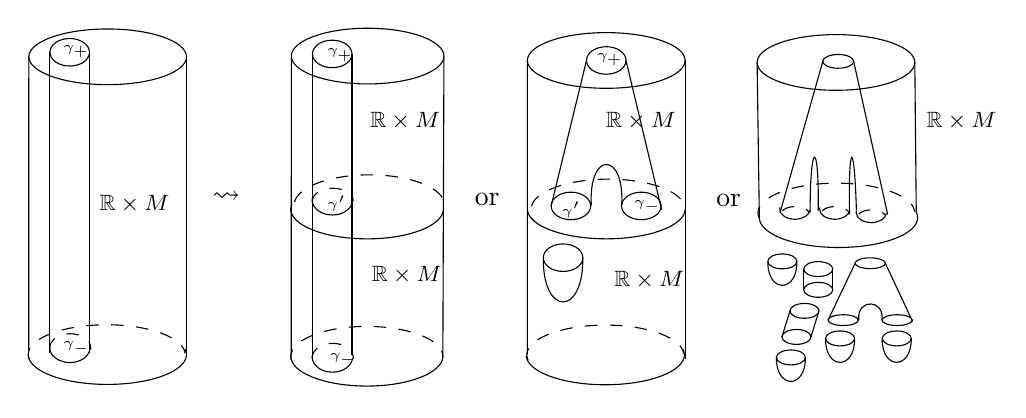
\begin{tikzpicture}[x=0.6pt,y=0.6pt,yscale=-1,xscale=1]
%uncomment if require: \path (0,300); %set diagram left start at 0, and has height of 300

%Shape: Ellipse [id:dp056395190934285244] 
\draw   (30.05,42.21) .. controls (30.05,32.95) and (51.31,25.44) .. (77.54,25.44) .. controls (103.76,25.44) and (125.02,32.95) .. (125.02,42.21) .. controls (125.02,51.48) and (103.76,58.98) .. (77.54,58.98) .. controls (51.31,58.98) and (30.05,51.48) .. (30.05,42.21) -- cycle ;
%Shape: Arc [id:dp6990177911205233] 
\draw  [draw opacity=0] (124.2,218.19) .. controls (124.74,219.28) and (125.02,220.4) .. (125.02,221.54) .. controls (125.02,231.47) and (103.68,239.51) .. (77.36,239.51) .. controls (51.54,239.51) and (30.52,231.77) .. (29.72,222.11) -- (77.36,221.54) -- cycle ; \draw   (124.2,218.19) .. controls (124.74,219.28) and (125.02,220.4) .. (125.02,221.54) .. controls (125.02,231.47) and (103.68,239.51) .. (77.36,239.51) .. controls (51.54,239.51) and (30.52,231.77) .. (29.72,222.11) ;  
%Straight Lines [id:da0017531833743447134] 
\draw    (30.05,41.97) -- (30.01,219.17) ;
%Straight Lines [id:da06191856902561077] 
\draw    (125.02,42.21) -- (125.02,221.93) ;
%Shape: Arc [id:dp7515744636820547] 
\draw  [draw opacity=0][dash pattern={on 4.5pt off 4.5pt}] (30.51,224.86) .. controls (29.98,223.78) and (29.7,222.67) .. (29.7,221.54) .. controls (29.7,211.61) and (50.85,203.57) .. (76.94,203.57) .. controls (102.32,203.57) and (123.02,211.19) .. (124.12,220.74) -- (76.94,221.54) -- cycle ; \draw  [dash pattern={on 4.5pt off 4.5pt}] (30.51,224.86) .. controls (29.98,223.78) and (29.7,222.67) .. (29.7,221.54) .. controls (29.7,211.61) and (50.85,203.57) .. (76.94,203.57) .. controls (102.32,203.57) and (123.02,211.19) .. (124.12,220.74) ;  
%Shape: Ellipse [id:dp170371749578063] 
\draw   (42.78,39.48) .. controls (42.78,34.9) and (48.11,31.19) .. (54.68,31.19) .. controls (61.25,31.19) and (66.58,34.9) .. (66.58,39.48) .. controls (66.58,44.06) and (61.25,47.77) .. (54.68,47.77) .. controls (48.11,47.77) and (42.78,44.06) .. (42.78,39.48) -- cycle ;
%Straight Lines [id:da7961683638948691] 
\draw    (42.78,39.48) -- (42.78,220.58) ;
%Straight Lines [id:da10134655093172151] 
\draw    (66.58,39.48) -- (66.58,220.58) ;
%Shape: Ellipse [id:dp0975147561159333] 
\draw   (188.15,41.77) .. controls (188.15,32.51) and (208.73,25) .. (234.11,25) .. controls (259.48,25) and (280.06,32.51) .. (280.06,41.77) .. controls (280.06,51.04) and (259.48,58.55) .. (234.11,58.55) .. controls (208.73,58.55) and (188.15,51.04) .. (188.15,41.77) -- cycle ;
%Shape: Arc [id:dp3077894307206215] 
\draw  [draw opacity=0] (279.39,222.94) .. controls (278.85,232.68) and (258.56,240.51) .. (233.6,240.51) .. controls (208.31,240.51) and (187.8,232.47) .. (187.8,222.54) .. controls (187.8,221.51) and (188.02,220.51) .. (188.44,219.53) -- (233.6,222.54) -- cycle ; \draw   (279.39,222.94) .. controls (278.85,232.68) and (258.56,240.51) .. (233.6,240.51) .. controls (208.31,240.51) and (187.8,232.47) .. (187.8,222.54) .. controls (187.8,221.51) and (188.02,220.51) .. (188.44,219.53) ;  
%Straight Lines [id:da4345493582140463] 
\draw    (188.15,42.97) -- (188.11,220.17) ;
%Straight Lines [id:da7275152931898132] 
\draw    (280.06,41.77) -- (279.4,223.71) ;
%Shape: Arc [id:dp15000914940586108] 
\draw  [draw opacity=0][dash pattern={on 4.5pt off 4.5pt}] (188.53,225.76) .. controls (188.05,224.72) and (187.8,223.64) .. (187.8,222.54) .. controls (187.8,212.61) and (208.3,204.57) .. (233.6,204.57) .. controls (258.89,204.57) and (279.39,212.61) .. (279.39,222.54) .. controls (279.39,222.67) and (279.39,222.8) .. (279.38,222.92) -- (233.6,222.54) -- cycle ; \draw  [dash pattern={on 4.5pt off 4.5pt}] (188.53,225.76) .. controls (188.05,224.72) and (187.8,223.64) .. (187.8,222.54) .. controls (187.8,212.61) and (208.3,204.57) .. (233.6,204.57) .. controls (258.89,204.57) and (279.39,212.61) .. (279.39,222.54) .. controls (279.39,222.67) and (279.39,222.8) .. (279.38,222.92) ;  
%Shape: Ellipse [id:dp7257031377511021] 
\draw   (200.88,40.48) .. controls (200.88,35.9) and (206.21,32.19) .. (212.78,32.19) .. controls (219.35,32.19) and (224.68,35.9) .. (224.68,40.48) .. controls (224.68,45.06) and (219.35,48.77) .. (212.78,48.77) .. controls (206.21,48.77) and (200.88,45.06) .. (200.88,40.48) -- cycle ;
%Straight Lines [id:da41430031772787657] 
\draw    (200.88,40.48) -- (200.88,221.58) ;
%Straight Lines [id:da8322496496190563] 
\draw    (224.68,40.48) -- (224.68,221.58) ;
%Shape: Arc [id:dp9948607311319655] 
\draw  [draw opacity=0] (279.72,134.27) .. controls (279.18,144.02) and (258.81,151.85) .. (233.76,151.85) .. controls (208.38,151.85) and (187.8,143.81) .. (187.8,133.88) .. controls (187.8,132.85) and (188.02,131.84) .. (188.45,130.86) -- (233.76,133.88) -- cycle ; \draw   (279.72,134.27) .. controls (279.18,144.02) and (258.81,151.85) .. (233.76,151.85) .. controls (208.38,151.85) and (187.8,143.81) .. (187.8,133.88) .. controls (187.8,132.85) and (188.02,131.84) .. (188.45,130.86) ;  
%Shape: Arc [id:dp47440163389587364] 
\draw  [draw opacity=0][dash pattern={on 4.5pt off 4.5pt}] (190.15,129.6) .. controls (192.26,120.45) and (211.6,113.29) .. (235.15,113.29) .. controls (260.12,113.29) and (280.35,121.34) .. (280.35,131.26) .. controls (280.35,132.27) and (280.14,133.26) .. (279.74,134.23) -- (235.15,131.26) -- cycle ; \draw  [dash pattern={on 4.5pt off 4.5pt}] (190.15,129.6) .. controls (192.26,120.45) and (211.6,113.29) .. (235.15,113.29) .. controls (260.12,113.29) and (280.35,121.34) .. (280.35,131.26) .. controls (280.35,132.27) and (280.14,133.26) .. (279.74,134.23) ;  
%Shape: Arc [id:dp6804839012339676] 
\draw  [draw opacity=0] (225.01,223.83) .. controls (224.48,228.48) and (219.25,232.13) .. (212.89,232.13) .. controls (206.17,232.13) and (200.72,228.07) .. (200.72,223.05) .. controls (200.72,222.56) and (200.77,222.07) .. (200.87,221.6) -- (212.89,223.05) -- cycle ; \draw   (225.01,223.83) .. controls (224.48,228.48) and (219.25,232.13) .. (212.89,232.13) .. controls (206.17,232.13) and (200.72,228.07) .. (200.72,223.05) .. controls (200.72,222.56) and (200.77,222.07) .. (200.87,221.6) ;  
%Shape: Arc [id:dp4500398352394417] 
\draw  [draw opacity=0][dash pattern={on 4.5pt off 4.5pt}] (200.83,224.21) .. controls (200.78,223.92) and (200.76,223.62) .. (200.76,223.33) .. controls (200.76,218.61) and (206.29,214.78) .. (213.11,214.78) .. controls (219.93,214.78) and (225.46,218.61) .. (225.46,223.33) .. controls (225.46,223.6) and (225.45,223.88) .. (225.41,224.15) -- (213.11,223.33) -- cycle ; \draw  [dash pattern={on 4.5pt off 4.5pt}] (200.83,224.21) .. controls (200.78,223.92) and (200.76,223.62) .. (200.76,223.33) .. controls (200.76,218.61) and (206.29,214.78) .. (213.11,214.78) .. controls (219.93,214.78) and (225.46,218.61) .. (225.46,223.33) .. controls (225.46,223.6) and (225.45,223.88) .. (225.41,224.15) ;  
%Shape: Arc [id:dp10273519473058612] 
\draw  [draw opacity=0] (224.88,126.86) .. controls (225,127.36) and (225.05,127.88) .. (225.05,128.4) .. controls (225.05,133.42) and (219.61,137.48) .. (212.89,137.48) .. controls (206.17,137.48) and (200.72,133.42) .. (200.72,128.4) .. controls (200.72,127.91) and (200.77,127.42) .. (200.87,126.95) -- (212.89,128.4) -- cycle ; \draw   (224.88,126.86) .. controls (225,127.36) and (225.05,127.88) .. (225.05,128.4) .. controls (225.05,133.42) and (219.61,137.48) .. (212.89,137.48) .. controls (206.17,137.48) and (200.72,133.42) .. (200.72,128.4) .. controls (200.72,127.91) and (200.77,127.42) .. (200.87,126.95) ;  
%Shape: Arc [id:dp9560702304930155] 
\draw  [draw opacity=0][dash pattern={on 4.5pt off 4.5pt}] (200.84,130.15) .. controls (200.79,129.87) and (200.76,129.57) .. (200.76,129.28) .. controls (200.76,124.89) and (206.29,121.33) .. (213.11,121.33) .. controls (219.82,121.33) and (225.28,124.77) .. (225.46,129.06) -- (213.11,129.28) -- cycle ; \draw  [dash pattern={on 4.5pt off 4.5pt}] (200.84,130.15) .. controls (200.79,129.87) and (200.76,129.57) .. (200.76,129.28) .. controls (200.76,124.89) and (206.29,121.33) .. (213.11,121.33) .. controls (219.82,121.33) and (225.28,124.77) .. (225.46,129.06) ;  
%Shape: Arc [id:dp7266228856012471] 
\draw  [draw opacity=0] (66.91,218.04) .. controls (66.38,222.69) and (61.16,226.34) .. (54.79,226.34) .. controls (48.07,226.34) and (42.62,222.27) .. (42.62,217.26) .. controls (42.62,216.76) and (42.67,216.28) .. (42.78,215.81) -- (54.79,217.26) -- cycle ; \draw   (66.91,218.04) .. controls (66.38,222.69) and (61.16,226.34) .. (54.79,226.34) .. controls (48.07,226.34) and (42.62,222.27) .. (42.62,217.26) .. controls (42.62,216.76) and (42.67,216.28) .. (42.78,215.81) ;  
%Shape: Arc [id:dp3689040331833249] 
\draw  [draw opacity=0][dash pattern={on 4.5pt off 4.5pt}] (42.73,218.41) .. controls (42.68,218.12) and (42.66,217.83) .. (42.66,217.53) .. controls (42.66,212.81) and (48.19,208.99) .. (55.01,208.99) .. controls (61.84,208.99) and (67.37,212.81) .. (67.37,217.53) .. controls (67.37,217.81) and (67.35,218.08) .. (67.31,218.35) -- (55.01,217.53) -- cycle ; \draw  [dash pattern={on 4.5pt off 4.5pt}] (42.73,218.41) .. controls (42.68,218.12) and (42.66,217.83) .. (42.66,217.53) .. controls (42.66,212.81) and (48.19,208.99) .. (55.01,208.99) .. controls (61.84,208.99) and (67.37,212.81) .. (67.37,217.53) .. controls (67.37,217.81) and (67.35,218.08) .. (67.31,218.35) ;  
%Shape: Ellipse [id:dp0661139858681199] 
\draw   (330.32,44.41) .. controls (330.32,35.15) and (351.58,27.64) .. (377.81,27.64) .. controls (404.03,27.64) and (425.29,35.15) .. (425.29,44.41) .. controls (425.29,53.67) and (404.03,61.18) .. (377.81,61.18) .. controls (351.58,61.18) and (330.32,53.67) .. (330.32,44.41) -- cycle ;
%Shape: Arc [id:dp8033107315109083] 
\draw  [draw opacity=0] (424.04,218.39) .. controls (424.58,219.47) and (424.87,220.59) .. (424.87,221.74) .. controls (424.87,231.66) and (403.53,239.71) .. (377.21,239.71) .. controls (351.39,239.71) and (330.36,231.97) .. (329.57,222.3) -- (377.21,221.74) -- cycle ; \draw   (424.04,218.39) .. controls (424.58,219.47) and (424.87,220.59) .. (424.87,221.74) .. controls (424.87,231.66) and (403.53,239.71) .. (377.21,239.71) .. controls (351.39,239.71) and (330.36,231.97) .. (329.57,222.3) ;  
%Straight Lines [id:da09066507708598825] 
\draw    (330.32,44.41) -- (330.28,221.6) ;
%Straight Lines [id:da3413965171016031] 
\draw    (425.29,44.41) -- (425.29,224.13) ;
%Shape: Arc [id:dp36547829111768615] 
\draw  [draw opacity=0][dash pattern={on 4.5pt off 4.5pt}] (330.78,225.06) .. controls (330.25,223.98) and (329.97,222.87) .. (329.97,221.74) .. controls (329.97,211.81) and (351.12,203.77) .. (377.21,203.77) .. controls (402.59,203.77) and (423.3,211.38) .. (424.39,220.94) -- (377.21,221.74) -- cycle ; \draw  [dash pattern={on 4.5pt off 4.5pt}] (330.78,225.06) .. controls (330.25,223.98) and (329.97,222.87) .. (329.97,221.74) .. controls (329.97,211.81) and (351.12,203.77) .. (377.21,203.77) .. controls (402.59,203.77) and (423.3,211.38) .. (424.39,220.94) ;  
%Shape: Ellipse [id:dp8629704518272938] 
\draw   (365.91,44.41) .. controls (365.91,39.83) and (371.24,36.12) .. (377.81,36.12) .. controls (384.38,36.12) and (389.71,39.83) .. (389.71,44.41) .. controls (389.71,48.99) and (384.38,52.7) .. (377.81,52.7) .. controls (371.24,52.7) and (365.91,48.99) .. (365.91,44.41) -- cycle ;
%Straight Lines [id:da8452678956957251] 
\draw    (365.91,44.41) -- (344.63,132.03) ;
%Straight Lines [id:da19999367359767395] 
\draw    (389.71,44.41) -- (411.17,134.3) ;
%Curve Lines [id:da16572232996503655] 
\draw    (368.81,131.66) .. controls (366.95,98.15) and (389.34,99.35) .. (387.05,132.03) ;
%Shape: Arc [id:dp6457528380286801] 
\draw  [draw opacity=0] (425.29,134.26) .. controls (424.72,144) and (403.68,151.83) .. (377.8,151.83) .. controls (351.71,151.83) and (330.53,143.87) .. (330.3,134.01) -- (377.8,133.85) -- cycle ; \draw   (425.29,134.26) .. controls (424.72,144) and (403.68,151.83) .. (377.8,151.83) .. controls (351.71,151.83) and (330.53,143.87) .. (330.3,134.01) ;  
%Shape: Arc [id:dp19216152259248287] 
\draw  [draw opacity=0][dash pattern={on 4.5pt off 4.5pt}] (332.81,132.15) .. controls (335.03,123.02) and (354.84,115.88) .. (378.95,115.88) .. controls (403.7,115.88) and (423.92,123.41) .. (425.23,132.88) -- (378.95,133.85) -- cycle ; \draw  [dash pattern={on 4.5pt off 4.5pt}] (332.81,132.15) .. controls (335.03,123.02) and (354.84,115.88) .. (378.95,115.88) .. controls (403.7,115.88) and (423.92,123.41) .. (425.23,132.88) ;  
%Shape: Ellipse [id:dp16448002790374439] 
\draw   (344.63,132.03) .. controls (344.63,127.45) and (349.95,123.74) .. (356.53,123.74) .. controls (363.1,123.74) and (368.43,127.45) .. (368.43,132.03) .. controls (368.43,136.61) and (363.1,140.32) .. (356.53,140.32) .. controls (349.95,140.32) and (344.63,136.61) .. (344.63,132.03) -- cycle ;
%Shape: Ellipse [id:dp9809662464110647] 
\draw   (387.05,132.03) .. controls (387.05,127.45) and (392.37,123.74) .. (398.94,123.74) .. controls (405.52,123.74) and (410.84,127.45) .. (410.84,132.03) .. controls (410.84,136.61) and (405.52,140.32) .. (398.94,140.32) .. controls (392.37,140.32) and (387.05,136.61) .. (387.05,132.03) -- cycle ;
%Shape: Ellipse [id:dp08366558813265468] 
\draw   (339.91,163.18) .. controls (339.91,158.6) and (345.24,154.89) .. (351.81,154.89) .. controls (358.39,154.89) and (363.71,158.6) .. (363.71,163.18) .. controls (363.71,167.76) and (358.39,171.47) .. (351.81,171.47) .. controls (345.24,171.47) and (339.91,167.76) .. (339.91,163.18) -- cycle ;
%Curve Lines [id:da09367632050515562] 
\draw    (339.91,163.18) .. controls (339.4,198.73) and (364.14,198.73) .. (363.71,163.18) ;
%Shape: Ellipse [id:dp8188508828087644] 
\draw   (468.66,45.61) .. controls (468.66,36.34) and (489.92,28.83) .. (516.14,28.83) .. controls (542.37,28.83) and (563.63,36.34) .. (563.63,45.61) .. controls (563.63,54.87) and (542.37,62.38) .. (516.14,62.38) .. controls (489.92,62.38) and (468.66,54.87) .. (468.66,45.61) -- cycle ;
%Shape: Arc [id:dp8117575286418532] 
\draw  [draw opacity=0] (564.51,135.73) .. controls (565.05,136.81) and (565.33,137.93) .. (565.33,139.08) .. controls (565.33,149) and (543.99,157.05) .. (517.67,157.05) .. controls (491.85,157.05) and (470.83,149.31) .. (470.04,139.64) -- (517.67,139.08) -- cycle ; \draw   (564.51,135.73) .. controls (565.05,136.81) and (565.33,137.93) .. (565.33,139.08) .. controls (565.33,149) and (543.99,157.05) .. (517.67,157.05) .. controls (491.85,157.05) and (470.83,149.31) .. (470.04,139.64) ;  
%Straight Lines [id:da331799661099899] 
\draw    (468.66,45.37) -- (470.01,139.6) ;
%Straight Lines [id:da9563297554519652] 
\draw    (563.63,45.61) -- (564.51,135.73) ;
%Shape: Arc [id:dp08014198609210887] 
\draw  [draw opacity=0][dash pattern={on 4.5pt off 4.5pt}] (470.01,139.6) .. controls (469.48,138.52) and (469.21,137.41) .. (469.21,136.28) .. controls (469.21,126.35) and (490.35,118.31) .. (516.44,118.31) .. controls (541.82,118.31) and (562.53,125.92) .. (563.63,135.48) -- (516.44,136.28) -- cycle ; \draw  [dash pattern={on 4.5pt off 4.5pt}] (470.01,139.6) .. controls (469.48,138.52) and (469.21,137.41) .. (469.21,136.28) .. controls (469.21,126.35) and (490.35,118.31) .. (516.44,118.31) .. controls (541.82,118.31) and (562.53,125.92) .. (563.63,135.48) ;  
%Shape: Ellipse [id:dp11318015897818423] 
\draw   (508.22,44.95) .. controls (508.22,42.66) and (512.38,40.81) .. (517.51,40.81) .. controls (522.64,40.81) and (526.8,42.66) .. (526.8,44.95) .. controls (526.8,47.24) and (522.64,49.09) .. (517.51,49.09) .. controls (512.38,49.09) and (508.22,47.24) .. (508.22,44.95) -- cycle ;
%Shape: Arc [id:dp5481702992712509] 
\draw  [draw opacity=0] (546.51,136.57) .. controls (546.06,139.65) and (542.17,142.05) .. (537.43,142.05) .. controls (532.39,142.05) and (528.31,139.34) .. (528.31,135.99) .. controls (528.31,135.62) and (528.36,135.25) .. (528.46,134.9) -- (537.43,135.99) -- cycle ; \draw   (546.51,136.57) .. controls (546.06,139.65) and (542.17,142.05) .. (537.43,142.05) .. controls (532.39,142.05) and (528.31,139.34) .. (528.31,135.99) .. controls (528.31,135.62) and (528.36,135.25) .. (528.46,134.9) ;  
%Shape: Arc [id:dp03984534439684717] 
\draw  [draw opacity=0][dash pattern={on 4.5pt off 4.5pt}] (529.88,136.9) .. controls (531.49,135.39) and (534.33,134.38) .. (537.57,134.38) .. controls (541.2,134.38) and (544.33,135.64) .. (545.79,137.47) -- (537.57,139.78) -- cycle ; \draw  [dash pattern={on 4.5pt off 4.5pt}] (529.88,136.9) .. controls (531.49,135.39) and (534.33,134.38) .. (537.57,134.38) .. controls (541.2,134.38) and (544.33,135.64) .. (545.79,137.47) ;  
%Straight Lines [id:da3617949510353735] 
\draw    (508.22,44.95) -- (482.46,136.1) ;
%Straight Lines [id:da649340590604436] 
\draw    (526.8,44.95) -- (547.3,137.17) ;
%Curve Lines [id:da8727790296078328] 
\draw    (500.59,136) .. controls (500.55,91.73) and (506.07,91.73) .. (505.46,134.9) ;
%Curve Lines [id:da4875409262510293] 
\draw    (524.3,137.17) .. controls (523.55,91.73) and (527.23,91.73) .. (528.46,134.9) ;
%Shape: Ellipse [id:dp7111828464384535] 
\draw   (475.13,165.41) .. controls (475.13,162.93) and (479.04,160.93) .. (483.87,160.93) .. controls (488.7,160.93) and (492.61,162.93) .. (492.61,165.41) .. controls (492.61,167.89) and (488.7,169.89) .. (483.87,169.89) .. controls (479.04,169.89) and (475.13,167.89) .. (475.13,165.41) -- cycle ;
%Curve Lines [id:da9672709945361355] 
\draw    (475.13,165.41) .. controls (474.75,184.63) and (492.92,184.63) .. (492.61,165.41) ;
%Shape: Ellipse [id:dp8770495266103071] 
\draw   (496.76,170.05) .. controls (496.76,167.57) and (500.67,165.56) .. (505.5,165.56) .. controls (510.33,165.56) and (514.24,167.57) .. (514.24,170.05) .. controls (514.24,172.52) and (510.33,174.53) .. (505.5,174.53) .. controls (500.67,174.53) and (496.76,172.52) .. (496.76,170.05) -- cycle ;
%Shape: Ellipse [id:dp4700005658957731] 
\draw   (496.76,182.56) .. controls (496.76,180.08) and (500.67,178.07) .. (505.5,178.07) .. controls (510.33,178.07) and (514.24,180.08) .. (514.24,182.56) .. controls (514.24,185.03) and (510.33,187.04) .. (505.5,187.04) .. controls (500.67,187.04) and (496.76,185.03) .. (496.76,182.56) -- cycle ;
%Shape: Ellipse [id:dp3742015758632733] 
\draw   (488.45,195.21) .. controls (488.45,192.74) and (492.36,190.73) .. (497.19,190.73) .. controls (502.01,190.73) and (505.93,192.74) .. (505.93,195.21) .. controls (505.93,197.69) and (502.01,199.69) .. (497.19,199.69) .. controls (492.36,199.69) and (488.45,197.69) .. (488.45,195.21) -- cycle ;
%Shape: Ellipse [id:dp05712935955362908] 
\draw   (483.6,210.9) .. controls (483.6,208.43) and (487.51,206.42) .. (492.34,206.42) .. controls (497.16,206.42) and (501.08,208.43) .. (501.08,210.9) .. controls (501.08,213.38) and (497.16,215.39) .. (492.34,215.39) .. controls (487.51,215.39) and (483.6,213.38) .. (483.6,210.9) -- cycle ;
%Straight Lines [id:da2384391731418305] 
\draw    (496.76,170.05) -- (496.76,182.56) ;
%Straight Lines [id:da33392656495348927] 
\draw    (514.24,170.05) -- (514.24,182.56) ;
%Straight Lines [id:da566045394847106] 
\draw    (505.93,195.21) -- (501.08,210.9) ;
%Straight Lines [id:da5614446278591068] 
\draw    (488.45,195.21) -- (483.6,210.9) ;
%Shape: Ellipse [id:dp035227786182282506] 
\draw   (480.27,223.26) .. controls (480.27,220.78) and (484.18,218.77) .. (489.01,218.77) .. controls (493.84,218.77) and (497.75,220.78) .. (497.75,223.26) .. controls (497.75,225.73) and (493.84,227.74) .. (489.01,227.74) .. controls (484.18,227.74) and (480.27,225.73) .. (480.27,223.26) -- cycle ;
%Curve Lines [id:da7379429542962657] 
\draw    (480.27,223.26) .. controls (479.89,242.47) and (498.06,242.47) .. (497.75,223.26) ;
%Shape: Ellipse [id:dp5542296065150325] 
\draw   (509.9,211.8) .. controls (509.9,209.33) and (513.82,207.32) .. (518.64,207.32) .. controls (523.47,207.32) and (527.38,209.33) .. (527.38,211.8) .. controls (527.38,214.28) and (523.47,216.29) .. (518.64,216.29) .. controls (513.82,216.29) and (509.9,214.28) .. (509.9,211.8) -- cycle ;
%Curve Lines [id:da7423459609744811] 
\draw    (509.9,211.8) .. controls (509.53,231.02) and (527.7,231.02) .. (527.38,211.8) ;
%Shape: Ellipse [id:dp24342029029087775] 
\draw   (544,211.8) .. controls (544,209.33) and (547.91,207.32) .. (552.74,207.32) .. controls (557.56,207.32) and (561.48,209.33) .. (561.48,211.8) .. controls (561.48,214.28) and (557.56,216.29) .. (552.74,216.29) .. controls (547.91,216.29) and (544,214.28) .. (544,211.8) -- cycle ;
%Curve Lines [id:da21595115366288664] 
\draw    (544,211.8) .. controls (543.62,231.02) and (561.79,231.02) .. (561.48,211.8) ;
%Shape: Ellipse [id:dp9507589820584572] 
\draw   (527.68,166.53) .. controls (527.68,164.74) and (531.76,163.28) .. (536.79,163.28) .. controls (541.82,163.28) and (545.9,164.74) .. (545.9,166.53) .. controls (545.9,168.32) and (541.82,169.77) .. (536.79,169.77) .. controls (531.76,169.77) and (527.68,168.32) .. (527.68,166.53) -- cycle ;
%Straight Lines [id:da7901347005685313] 
\draw    (527.68,166.53) -- (511.39,200.8) ;
%Straight Lines [id:da056288864133154926] 
\draw    (545.9,166.53) -- (562.33,201.69) ;
%Curve Lines [id:da988145377883118] 
\draw    (529.9,200.65) .. controls (528.48,187.55) and (545.61,188.02) .. (543.86,200.8) ;
%Shape: Ellipse [id:dp23604569535188302] 
\draw   (511.39,200.8) .. controls (511.39,199.01) and (515.47,197.55) .. (520.5,197.55) .. controls (525.53,197.55) and (529.61,199.01) .. (529.61,200.8) .. controls (529.61,202.59) and (525.53,204.04) .. (520.5,204.04) .. controls (515.47,204.04) and (511.39,202.59) .. (511.39,200.8) -- cycle ;
%Shape: Ellipse [id:dp7261778653447537] 
\draw   (543.86,200.8) .. controls (543.86,199.01) and (547.94,197.55) .. (552.97,197.55) .. controls (558,197.55) and (562.08,199.01) .. (562.08,200.8) .. controls (562.08,202.59) and (558,204.04) .. (552.97,204.04) .. controls (547.94,204.04) and (543.86,202.59) .. (543.86,200.8) -- cycle ;
%Shape: Arc [id:dp3746223374313047] 
\draw  [draw opacity=0] (524.51,134.57) .. controls (524.06,137.65) and (520.17,140.05) .. (515.43,140.05) .. controls (510.39,140.05) and (506.31,137.34) .. (506.31,133.99) .. controls (506.31,133.62) and (506.36,133.25) .. (506.46,132.9) -- (515.43,133.99) -- cycle ; \draw   (524.51,134.57) .. controls (524.06,137.65) and (520.17,140.05) .. (515.43,140.05) .. controls (510.39,140.05) and (506.31,137.34) .. (506.31,133.99) .. controls (506.31,133.62) and (506.36,133.25) .. (506.46,132.9) ;  
%Shape: Arc [id:dp21450518339030733] 
\draw  [draw opacity=0][dash pattern={on 4.5pt off 4.5pt}] (507.88,134.9) .. controls (509.49,133.39) and (512.33,132.38) .. (515.57,132.38) .. controls (519.2,132.38) and (522.33,133.64) .. (523.79,135.47) -- (515.57,137.78) -- cycle ; \draw  [dash pattern={on 4.5pt off 4.5pt}] (507.88,134.9) .. controls (509.49,133.39) and (512.33,132.38) .. (515.57,132.38) .. controls (519.2,132.38) and (522.33,133.64) .. (523.79,135.47) ;  
%Shape: Arc [id:dp37481817018727304] 
\draw  [draw opacity=0] (500.51,134.57) .. controls (500.06,137.65) and (496.17,140.05) .. (491.43,140.05) .. controls (486.39,140.05) and (482.31,137.34) .. (482.31,133.99) .. controls (482.31,133.62) and (482.36,133.25) .. (482.46,132.9) -- (491.43,133.99) -- cycle ; \draw   (500.51,134.57) .. controls (500.06,137.65) and (496.17,140.05) .. (491.43,140.05) .. controls (486.39,140.05) and (482.31,137.34) .. (482.31,133.99) .. controls (482.31,133.62) and (482.36,133.25) .. (482.46,132.9) ;  
%Shape: Arc [id:dp03724951552805966] 
\draw  [draw opacity=0][dash pattern={on 4.5pt off 4.5pt}] (483.88,134.9) .. controls (485.49,133.39) and (488.33,132.38) .. (491.57,132.38) .. controls (495.2,132.38) and (498.33,133.64) .. (499.79,135.47) -- (491.57,137.78) -- cycle ; \draw  [dash pattern={on 4.5pt off 4.5pt}] (483.88,134.9) .. controls (485.49,133.39) and (488.33,132.38) .. (491.57,132.38) .. controls (495.2,132.38) and (498.33,133.64) .. (499.79,135.47) ;  

% Text Node
\draw (139.08,121.83) node [anchor=north west][inner sep=0.75pt]    {$\rightsquigarrow $};
% Text Node
\draw (71.12,123.83) node [anchor=north west][inner sep=0.75pt]  [font=\footnotesize]  {$\mathbb{R} \times M$};
% Text Node
\draw (208.07,35.68) node [anchor=north west][inner sep=0.75pt]  [font=\tiny]  {$\gamma _{+}$};
% Text Node
\draw (49.15,212.24) node [anchor=north west][inner sep=0.75pt]  [font=\tiny]  {$\gamma _{-}$};
% Text Node
\draw (209.61,219.23) node [anchor=north west][inner sep=0.75pt]  [font=\tiny]  {$\gamma _{-}$};
% Text Node
\draw (208.07,124.24) node [anchor=north west][inner sep=0.75pt]  [font=\tiny]  {$\gamma '$};
% Text Node
\draw (297.07,122.73) node [anchor=north west][inner sep=0.75pt]   [align=left] {or};
% Text Node
\draw (49.15,33.72) node [anchor=north west][inner sep=0.75pt]  [font=\tiny]  {$\gamma _{+}$};
% Text Node
\draw (392.94,127.04) node [anchor=north west][inner sep=0.75pt]  [font=\tiny]  {$\gamma _{-}$};
% Text Node
\draw (349.35,128.14) node [anchor=north west][inner sep=0.75pt]  [font=\tiny]  {$\gamma '$};
% Text Node
\draw (370.56,38.38) node [anchor=north west][inner sep=0.75pt]  [font=\tiny]  {$\gamma _{+}$};
% Text Node
\draw (442.53,123.33) node [anchor=north west][inner sep=0.75pt]   [align=left] {or};
% Text Node
\draw (235.12,166.83) node [anchor=north west][inner sep=0.75pt]  [font=\footnotesize]  {$\mathbb{R} \times M$};
% Text Node
\draw (234.12,73.83) node [anchor=north west][inner sep=0.75pt]  [font=\footnotesize]  {$\mathbb{R} \times M$};
% Text Node
\draw (376.12,73.83) node [anchor=north west][inner sep=0.75pt]  [font=\footnotesize]  {$\mathbb{R} \times M$};
% Text Node
\draw (381.12,169.83) node [anchor=north west][inner sep=0.75pt]  [font=\footnotesize]  {$\mathbb{R} \times M$};
% Text Node
\draw (569.12,73.83) node [anchor=north west][inner sep=0.75pt]  [font=\footnotesize]  {$\mathbb{R} \times M$};


\end{tikzpicture}

\end{center}

where for the rightmost diagram, each of the bottom components is a map to $\mathbb{R}^n$.

\begin{definition}

Let $(F,j)$ be a Riemann surface, $\dot{F}=F$ a finite subset, and $u:(\dot{F},j)\stackrel{J-\text{holomorphic}}{\to} (\mathbb{R}\times M, J)$. Then the \textbf{Hofer energy} is
\[
E(u)=\sup_{\phi \in \mathcal{C}} \int_{\dot{F}} u^* d(\phi, \alpha)
\]
where
\[
\mathcal{C} = \left\{ \phi: \mathbb{R} \to [1,2] \mid
\begin{cases}
\phi(s) = 1 & \text{if } s \ll 0, \\
\phi(s) = 2 & \text{if } s \gg 0, \\
\phi'(s) \ge 0 & \text{for all } s \in \mathbb{R}
\end{cases}
\right\}
\]

\end{definition}

\begin{proposition}

\begin{align*}
E(u)&= 2\sum_{i=1}^{k_+} \mathcal{A}(\gamma_{+,i})-\sum_{i=1}^{k_-} \mathcal{A}(\gamma_{-,i}) \\
&\ge 0.
\end{align*}

\end{proposition}

\section{Grading}

\begin{theorem}

If $u: (\dot{E}, j)\to \mathbb{R}\times M$ is $J$-holomorphic, the following are equivalent:
\begin{itemize}
\item $E(u)<\infty$
\item For any puncture $p$ of $\dot{F}$, either $p$ is removable or $u$ converges to some Reeb orbit along $P$.
\end{itemize}

\end{theorem}

Assume the $H_1(M; \mathbb{Z})$ is torsion free. If $H_1(M)=0$, then for each Reeb orbit $\gamma$, fix a surface $F_\gamma \subset M$ spanning $\gamma$. If $H_1(M; \mathbb{Z})\neq 0$, choose a basis of $H_1(M)$ and represent it by oriented curves $c_1,...c_k$. Choose a trivialization of $\xi/c_1$. For any Reeb orbit $\gamma$, choose $F_\gamma$ such that $[\partial F_\gamma]=[\gamma]-\sum n_i [c_i]$. Choose a trivialization of $\xi \mid_{\gamma}$ so that it extends over $F_\gamma$ and agrees with the trivialization of $\xi/c_i$. This defines a Conley-Zehder index for each $\gamma$.

For each $J$-holomorphic cylinder $u$, we can attach $F_{\gamma_+}$ and $F_{\gamma_-}$:
\begin{center}
\tikzset{every picture/.style={line width=0.75pt}} %set default line width to 0.75pt        

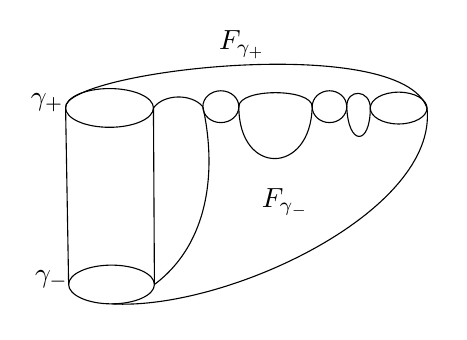
\begin{tikzpicture}[x=0.5pt,y=0.5pt,yscale=-1,xscale=1]
%uncomment if require: \path (0,300); %set diagram left start at 0, and has height of 300

%Shape: Ellipse [id:dp8909013950100437] 
\draw   (85,82) .. controls (85,74.27) and (99.21,68) .. (116.75,68) .. controls (134.29,68) and (148.5,74.27) .. (148.5,82) .. controls (148.5,89.73) and (134.29,96) .. (116.75,96) .. controls (99.21,96) and (85,89.73) .. (85,82) -- cycle ;
%Straight Lines [id:da939999364801372] 
\draw    (85,82) -- (87.2,209.6) ;
%Straight Lines [id:da32030547024849] 
\draw    (148.5,82) -- (149.2,209.6) ;
%Shape: Ellipse [id:dp22593738557210807] 
\draw   (87.2,209.6) .. controls (87.2,201.87) and (101.08,195.6) .. (118.2,195.6) .. controls (135.32,195.6) and (149.2,201.87) .. (149.2,209.6) .. controls (149.2,217.33) and (135.32,223.6) .. (118.2,223.6) .. controls (101.08,223.6) and (87.2,217.33) .. (87.2,209.6) -- cycle ;
%Shape: Ellipse [id:dp3903650035201627] 
\draw   (184.2,81.1) .. controls (184.2,74.75) and (190.02,69.6) .. (197.2,69.6) .. controls (204.38,69.6) and (210.2,74.75) .. (210.2,81.1) .. controls (210.2,87.45) and (204.38,92.6) .. (197.2,92.6) .. controls (190.02,92.6) and (184.2,87.45) .. (184.2,81.1) -- cycle ;
%Shape: Ellipse [id:dp439043297167095] 
\draw   (263.2,81.1) .. controls (263.2,74.75) and (268.8,69.6) .. (275.7,69.6) .. controls (282.6,69.6) and (288.2,74.75) .. (288.2,81.1) .. controls (288.2,87.45) and (282.6,92.6) .. (275.7,92.6) .. controls (268.8,92.6) and (263.2,87.45) .. (263.2,81.1) -- cycle ;
%Shape: Ellipse [id:dp5515211986371753] 
\draw   (305.2,82.1) .. controls (305.2,75.75) and (314.38,70.6) .. (325.7,70.6) .. controls (337.02,70.6) and (346.2,75.75) .. (346.2,82.1) .. controls (346.2,88.45) and (337.02,93.6) .. (325.7,93.6) .. controls (314.38,93.6) and (305.2,88.45) .. (305.2,82.1) -- cycle ;
%Curve Lines [id:da43171084391564163] 
\draw    (118.2,223.6) .. controls (201.2,228.6) and (354.2,156.6) .. (346.2,82.1) ;
%Curve Lines [id:da12535479193092525] 
\draw    (85,82) .. controls (82.2,55.6) and (327.2,26.6) .. (346.2,82.1) ;
%Curve Lines [id:da515259067066461] 
\draw    (288.2,81.1) .. controls (289.2,109.6) and (305.2,109.6) .. (305.2,82.1) ;
%Curve Lines [id:da3208943864453322] 
\draw    (210.2,81.1) .. controls (210.2,131.6) and (262.2,130.6) .. (263.2,81.1) ;
%Curve Lines [id:da7762191468457265] 
\draw    (210.2,81.1) .. controls (210.2,67.6) and (263.2,67.6) .. (263.2,81.1) ;
%Curve Lines [id:da23187615015116236] 
\draw    (288.2,81.1) .. controls (288.2,67.6) and (305.2,68.6) .. (305.2,82.1) ;
%Curve Lines [id:da3836381595978182] 
\draw    (148.5,82) .. controls (156.2,71.6) and (176.2,71.6) .. (184.2,81.1) ;
%Curve Lines [id:da3396096780840039] 
\draw    (149.2,209.6) .. controls (189.2,179.6) and (194.2,126.6) .. (184.2,81.1) ;

% Text Node
\draw (58,69.4) node [anchor=north west][inner sep=0.75pt]    {$\gamma _{+}$};
% Text Node
\draw (61,197.4) node [anchor=north west][inner sep=0.75pt]    {$\gamma _{-}$};
% Text Node
\draw (194,24.4) node [anchor=north west][inner sep=0.75pt]    {$F_{\gamma _{+}}$};
% Text Node
\draw (225,138.4) node [anchor=north west][inner sep=0.75pt]    {$F_{\gamma _{-}}$};

\end{tikzpicture}
\end{center}

which gives an element in $H_2(M)$.

Assume does not exist a contractible Reeb orbits. We define a chain complex $(C_*, \partial)$ where $C_*$ is a free $\mathbb{Q}[H_2(M)]$ module generated by all good Reeb orbits. For each $A\in H_2(M)$, $| A|  = -2 \langle c_1(\xi), A \rangle$, define $\partial_{\gamma_+}= \sum_{\gamma_-, A}\# \mathcal{M}(\gamma_+, \gamma_-, A) e^A \frac{1}{m(\gamma_-)}\gamma_-$ where $m(\gamma_-)$ is the multiplcity of $\gamma_-$. This gives $|\gamma_+| -| \gamma_- | -| A| =1$. Define $| \gamma| =\mu_{c_2}(\gamma)+n-3$.

\begin{definition}

$\gamma$ is \textbf{bad} if $\gamma$ is multiple cover of embedded $\gamma'$ and $\mu_{\text{cz}}(\gamma)-\mu_{\text{cz}}(\gamma')$ is odd.

\end{definition}

\begin{example}

For $\dim \mathcal{M}=3$, $\gamma$ is bad if and only if $\gamma$ is an even multiple cover of a negative hyperbolic one.

\end{example}

If there exists a contractible Reeb orbits:
\vspace{-20pt}
\begin{figure}[htbp]
  \centering
  \includegraphics[width=1\textwidth]{images/bao1.png}
  \label{fig:bi14}
\end{figure}
\vspace{-40pt} % Adjust this value to control the space

This gives the contact homology. One important variant of the contact homology is the (rational) symplectic field theory.

\begin{example}

In $\dim =3$, if $\gamma$ is hyperbolic, then
\[
\mu_{\text{cz}}(\gamma, k) = k \mu_{\text{cz}}(\gamma).
\]

Let $u$ be $J$-holomorphic. If $\text{ind }u = \mu(\gamma_+)-\mu(\gamma)-| A| $. If $u$ is $k$-fold cover of $u'$ and there are no elliptic orbits, then $\text{ind }u = k\cdot \text{ind }u'$.

If $u'$ transverses $\text{ind}$ and $\text{ind } u' \ge 1$, then $\text{ind }u \ge k$. In the definition of $\partial, \text{ind }(u)=1 \implies k=1$.

We can always eliminate elliptic orbits up to any action:
\begin{center}
    
\tikzset{every picture/.style={line width=0.75pt}} %set default line width to 0.75pt        

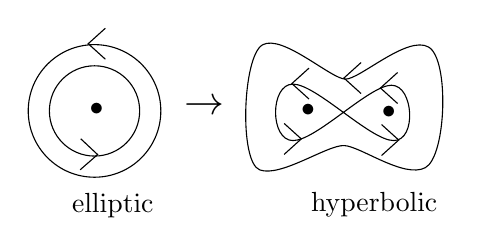
\begin{tikzpicture}[x=0.4pt,y=0.4pt,yscale=-1,xscale=1]
%uncomment if require: \path (0,300); %set diagram left start at 0, and has height of 300

%Shape: Circle [id:dp08144944578189617] 
\draw   (70.82,119.71) .. controls (70.82,86.63) and (97.63,59.82) .. (130.71,59.82) .. controls (163.79,59.82) and (190.6,86.63) .. (190.6,119.71) .. controls (190.6,152.79) and (163.79,179.6) .. (130.71,179.6) .. controls (97.63,179.6) and (70.82,152.79) .. (70.82,119.71) -- cycle ;
%Shape: Circle [id:dp39773554712775216] 
\draw   (89.93,119.71) .. controls (89.93,97.19) and (108.19,78.93) .. (130.71,78.93) .. controls (153.23,78.93) and (171.49,97.19) .. (171.49,119.71) .. controls (171.49,142.23) and (153.23,160.49) .. (130.71,160.49) .. controls (108.19,160.49) and (89.93,142.23) .. (89.93,119.71) -- cycle ;
%Shape: Polygon Curved [id:ds02793189593737866] 
\draw   (399,96.5) .. controls (419,96.5) and (422,146.5) .. (401,146.5) .. controls (380,146.5) and (331,95.5) .. (310,95.5) .. controls (289,95.5) and (289,146.5) .. (310,146.5) .. controls (331,146.5) and (379,96.5) .. (399,96.5) -- cycle ;
%Shape: Polygon Curved [id:ds03073014229495996] 
\draw   (357.5,91) .. controls (370.5,91) and (413.5,51) .. (432.5,62) .. controls (451.5,73) and (448.5,161) .. (429.5,171) .. controls (410.5,181) and (371.5,152) .. (356.5,151) .. controls (341.5,150) and (299,180) .. (280,173) .. controls (261,166) and (264.5,70) .. (282.5,60) .. controls (300.5,50) and (344.5,91) .. (357.5,91) -- cycle ;
\draw   (371.5,104) -- (356,90) -- (371.5,76) ;
\draw   (324.5,109) -- (309,95) -- (324.5,81) ;
\draw   (390,132) -- (405.5,146) -- (390,160) ;
\draw   (302,131) -- (317.5,145) -- (302,159) ;
\draw   (404.5,113) -- (389,99) -- (404.5,85) ;
\draw   (140.5,73) -- (125,59) -- (140.5,45) ;
\draw   (118.25,144.87) -- (133.5,159.14) -- (117.76,172.86) ;

% Text Node
\draw (124,110.4) node [anchor=north west][inner sep=0.75pt]    {$\bullet $};
% Text Node
\draw (315,111.4) node [anchor=north west][inner sep=0.75pt]    {$\bullet $};
% Text Node
\draw (388,113.4) node [anchor=north west][inner sep=0.75pt]    {$\bullet $};
% Text Node
\draw (210,107.4) node [anchor=north west][inner sep=0.75pt]  [font=\Large]  {$\rightarrow $};
% Text Node
\draw (108,192) node [anchor=north west][inner sep=0.75pt]   [align=left] {elliptic};
% Text Node
\draw (324,191) node [anchor=north west][inner sep=0.75pt]   [align=left] {hyperbolic};

\end{tikzpicture}

\end{center}

These two images have the same contact structure, but different contact forms.

\end{example}
\chapter{Global Kuranishi Charts: Construction}
\label{s3}
\abstract{Following Abouzaid–McLean–Smith 2021, we explain the construction of global Kuranishi charts for genus 0 Gromov–Witten moduli spaces and show that the outcome of the construction is unique up to equivalence. Time permitting, we will also briefly discuss how one can extend this construction to settings beyond genus 0 GW theory.}

\section{The AMS Trick}

Take $(X^{2n},\omega)$, $A\in H_2(X; \mathbb{Z})$, and $J$ an $\omega$-tame almost complex structure on $X$. This gives $\overline{\mathcal{M}}_0(X,A,J)$ which consists of $J$-holomorphic maps $u$ from trees of spheres $\Sigma$ to $X$ with $u_k[\Sigma]=A$.

\begin{theorem}
[Abouzaid, McLean, Smith, 2021]

$\overline{\mathcal{M}}_0(X,A,J)$ has a global Kuranishi chart, constructed often making some choices, but the resulting chart is unique up to equivalence.

\end{theorem}

\begin{proposition}

\[
\overline{\mathcal{M}}_0^*(\mathbb{CP}^d, d ) = \left\{ f: \Sigma \to \mathbb{CP}^d \mid f \text{ is a degree } d \text{ genus } 0 \text{ stable map and } f \text{ is non-degenerate} \right\}
\]

where non-degenerate means the image of $f$ is not contained in any hyperplane on $\mathbb{CP}^n$. Then there is a smooth quasi-projective variety of the expected dimension.

\end{proposition}

Here is an example of a non-degenerate function:

\begin{example}

\[\mathbb{CP}^1 \to \mathbb{CP}^d\]
\[[u,v]\mapsto [u^d; u^{d-1}v, ..., v^d]\]

\end{example}

The proposition gives rise to a nontrivial family

\[
\begin{tikzcd}
	{\mathcal{C}} & {\mathbb{CP}^d} \\
	{\overline{\mathcal{M}}_0^*(\mathbb{CP}^n, d)}
	\arrow[from=1-1, to=1-2]
	\arrow[from=1-1, to=2-1]
\end{tikzcd}
\]

where $\mathcal{C}$ is also a smooth, quasiprojective variety.

Every map $\mathcal{L}\to Z$ is induced with an embedding $Z\stackrel{[s_0:... ]}{\hookrightarrow} \mathbb{CP}^n$ where $s_0, ..., s_p \in H^0(Z; \mathcal{L})$ have no common zero.

Let's recall some basic definitions about ample line bundles.

\begin{definition}

$\mathcal{L}$ is \textbf{very ample} if $\exists s_0,...,s_n \in H^0(Z; \mathcal{L})$ such that we get an embedding $Z\stackrel{[s_0:...:s_n]}{\hookrightarrow} \mathbb{CP}^n$

\end{definition}

\begin{definition}

$ \mathcal{L}$ is \textbf{ample} if there exists $m>1$ such that $L^{\otimes m}$ is very ample.

\end{definition}

\begin{proposition}
    If $Z$ is a cone, then $\mathcal{L}$ is ample if and only if $\deg \mathcal{L}>0$ on each component of $Z$.
\end{proposition}

We can finally state the AMS trick:

\begin{lemma}
[AMS Trick]

Suppose $Z$ is a compact complex manifold $\mathcal{L}\to Z$ is an ample line bundle and $ \mathcal{E}\to Z$ is a holomorphic vector bundle, and endow everything with the Hermitian action. For $k\gg 1$, define
\[
W_k := \text{Im} \left( H^0(Z; \mathcal{E} \otimes \mathcal{L}^{\otimes k})\otimes_{\mathbb{C}} \overline{H^0(Z; \mathcal{L}^{\otimes k})} \stackrel{\langle \cdot, \cdot \rangle}{\longrightarrow} \Omega^0(Z, \mathcal{E})\right).
\]

As $k\to \infty$, $W_k$ provides an $L^2$ extension of $\Omega^0(Z, \mathcal{E})$, i.e. for all $\xi \in \Omega^0(Z, \mathcal{E}), \exists k\gg 1$ and $\eta \in W_k$ such that $\langle \xi, \eta \rangle_{L_2}\neq 0$.

\end{lemma}

\section{Construction}

\subsection{Line Bundles on $X$}

Approximate $\Omega$ by a symplectic form $\Omega$ which tames $J$ and satisfies $[\Omega] \in H^2(X; \mathbb{Q})$. Clear the denominator to get $[\Omega] \in H^2(X; \mathbb{Z})/\text{torsion}$ which implies that there exists a $C^\infty$ complex line bundle $L_\Omega \to X$ such that the first Chern class $c_1(L_\Omega)=[\Omega]$.

From Chern-Weil theory, we have the following lemma:

\begin{lemma}

There exists a Hermitian metric and a Hermitian connection $\nabla$ on $L_\Omega$ such that its curvature is $-2\pi i \Omega$.

\end{lemma}

Notation: $[\Omega]\cdot A=d$.

\subsection{Framed Genus 0 Curves }

Let's start with a (genus $0$) $J$-holomorphic stable $u:\Sigma\to X$. Then $u^*\mid_\Sigma \to \Sigma$ has a holomorphic structured generated by $(u^*\nabla)^{0,1}$. We know that $\int u^* \Omega \ge 0$ on each component of $\Sigma$ where $u$ is $J$-holomorphic and $\Omega$ tames $J$. We also know that $\int u^*\Omega >0$ on each unstable component. This implies that the line bundle $u^*L_\Omega$ has non-negative degree on each component $\Sigma$ and positive degree on each unstable component of $\Sigma$.

From last time, we know that
\[
\dim_{\mathbb{C}} H^0(\Sigma; u^*L_\Omega)=d+1, \\
H^1(\Sigma; u^* L_\Omega) = 0.
\]

Choose a basis $F=(f_0,...,f_d)$ of $H^0(\Sigma; u^*L_\Omega)$, called a \textbf{framing}. Consider the degree $d$ genus $0$ stable map
\[
\Sigma \stackrel{\Phi_F=[f_0:...:f_d]}{\longrightarrow} \mathbb{CP}^d
\]
Then $(\Sigma, \Phi_F) \in \overline{\mathcal{M}}_0^*(\mathbb{CP}^d, d)$. So we have

\[\begin{tikzcd}
	\Sigma & {\mathcal{C}} & {\mathbb{CP}^d} \\
	{(\Sigma, \Phi_F)} & {\overline{\mathcal{M}}_0^*(\mathbb{CP}^d, d)}
	\arrow["{{i_F}}", hook, from=1-1, to=1-2]
	\arrow[from=1-1, to=2-1]
	\arrow[from=1-2, to=1-3]
	\arrow[from=1-2, to=2-2]
	\arrow["\in"{description}, draw=none, from=2-1, to=2-2]
\end{tikzcd}\]

where $i_F$ is a embedding as a fiber.

We have
\[
H(\Sigma, u, F) = \left( \int_\Sigma \langle f_i, f_j \rangle u^*\Omega \right)_{0\le i, j \le d}
\]
is a Hermitian positive definite $(d+1)\times (d+1)$ matrix.

\begin{definition}

A \textbf{framed genus 0 curve in $X$} is a tuple $(\Sigma, u,F)$ where
\begin{enumerate}
\item $\Sigma$ is a nodal genus 0 curve.
\item $u: \Sigma \to X$ is a $C^\infty$ map in class $A$ such that $\int u^*\Omega \ge 0$ on each component of $\Sigma$ and $\int u^*\Omega > 0$ on each unstable component.
\item $F: (f_0,...,f_d)$ is a basis of $H^0(\Sigma; u^*L_\Omega)$ such that the matrix $H(\Sigma, u, F)$ is positive definite.
\end{enumerate}

\end{definition}

So $(\Sigma, u, F)\sim (\Sigma',u', F')$ if

\[\begin{tikzcd}
	\Sigma \\
	&& X \\
	{\Sigma'}
	\arrow["u", from=1-1, to=2-3]
	\arrow["\varphi"', from=1-1, to=3-1]
	\arrow["\cong", from=1-1, to=3-1]
	\arrow["{u'}"', from=3-1, to=2-3]
\end{tikzcd}\]
commutes.

\subsection{Achieving Transversality }

Choose
\begin{enumerate}
\item A relatively ample line bundle $\mathcal{L}$ on $\mathcal{C} \to \overline{\mathcal{M}}_0^* ( \mathbb{CP}^d, d)$ equipped with a Hermitian metric such that the natural $U(d+1)$ action on $\overline{\mathcal{M}}_0^*(\mathbb{CP}^d, d)$ lifts to an action of $\mathcal{L}$ and preserves the metric.
\item A $\mathbb{C}$-linear connection on $T^{*\text{ }0,1} \mathcal{C}$ which is an invariant under the $U(d+1)$ action.
\item A $\mathbb{C}$-linear connection on $TX$ (viewed as a $\mathbb{C}$-vector bundle on $J$)
\item A large integer $k\gg 1$.
\end{enumerate}

For more details, see [Horschi, Swaminathan, 2021, Section 2.1].

\begin{proposition}

The \textbf{thickening} $\mathcal{T}$ is the space of tuples $(\Sigma, u, F, \eta)$ where
\begin{enumerate}
\item $(\Sigma, u, F)$ is a framed genus $0$ curve in $X$
\item We have
    \[
    \eta \in H^0(\Sigma; u^*TX\otimes i_F^*(T^{* \text{ }0,1}\mathcal{C}\otimes \mathcal{L}^{\otimes k}))\otimes_{\mathbb{C}} \overline{H^0(\Sigma; i_F^* \mathcal{L}^{\otimes k})}
    \]
    satisfying the equation
    \[
    \overline{\partial}_J u + \langle \eta \rangle \circ di_F=0
    \]
\end{enumerate}

\end{proposition}

\begin{proposition}

The \textbf{obstruction bundle} $\mathcal{E}\to \mathcal{T}$ is a vector bundle whose fiber over $(\Sigma, u, F, \eta)$ is
\[
E_{(\Sigma, u, F)}\oplus \mathcal{H}_{d+1}
\]
where $\mathcal{H}_{d+1}$ is a space of $(d+1)\times (d+1)$ Hermitian matrices.

\end{proposition}

\begin{proposition}

The \textbf{obstruction section} is
\[
\mathcal{S}(\Sigma, u, F, \eta)=(\eta, \log \mathcal{H}(\Sigma, u, F)).
\]

\end{proposition}

\begin{proposition}

The \textbf{symmetry group} is
\[
G=U(d+1).
\]

\end{proposition}

The key point is that $\mathcal{T}$ is cut out transversally for $k\gg 1$ by the AMS trick.

%%%%%%%%%%%%%%%%%%%%%part.tex%%%%%%%%%%%%%%%%%%%%%%%%%%%%%%%%%%
% 
% sample part title
%
% Use this file as a template for your own input.
%
%%%%%%%%%%%%%%%%%%%%%%%% Springer %%%%%%%%%%%%%%%%%%%%%%%%%%

\begin{partbacktext}
\part{Talks}

There were ten talks:\\

\begin{enumerate}
    \item \href{#pieloch}{Alex Pieloch: Spectral Equivalence of Nearby Lagrangians}
    
    Fix a commutative ring spectrum $R$. In this talk, we will show that any nearby Lagrangian in a cotangent bundle of a closed manifold is equivalent in the wrapped Fukaya category with $R$-coefficients to an $R$-brane supported on the zero section. As an application, we impose topological restrictions on the embeddings of exact Lagrangian fillings of the standard Legendrian unknot in sub-critical Stein domains. This is joint work with Johan Asplund and Yash Deshmukh.

    \item \href{#cristofaro}{Dan Cristofaro-Gardiner: Low-Action Holomorphic Curves and Invariant Sets}
    
    I will discuss a new compactness theorem for sequences of low-action punctured holomorphic curves of controlled topology, in any dimension, without imposing the typical assumption of uniformly bounded Hofer energy; in the limit, we extract a family of closed Reeb-invariant subsets. I will also explain why such sequences exist in abundance in low-dimensional symplectic dynamics, via the theory of embedded contact homology. This has various applications: the one I want to focus on in my talk is a generalization to higher genus surfaces and three-manifolds of the celebrated Le Calvez–Yoccoz theorem. All of this is joint with Rohil Prasad.

    \item \href{#pomerleano}{Daniel Pomerleano: Homological Mirror Symmetry for Batyrev Mirror Pairs}
    
    I will survey a recent proof of a version of Kontsevich’s homological mirror symmetry conjecture for a large class of mirror pairs of Calabi–Yau hypersurfaces in toric varieties. These mirror pairs were constructed by Batyrev from dual reflexive polytopes. The theorem holds in characteristic zero and in all but finitely many positive characteristics. This is joint work with Ganatra, Hanlon, Hicks, and Sheridan.

    \item \href{#wang}{Luya Wang: Deformation Inequivalent Symplectic Structures and Donaldson's Four-Six Question}

    Studying symplectic structures up to deformation equivalences is a fundamental question in symplectic geometry. Donaldson asked: given two homeomorphic closed symplectic four-manifolds, are they diffeomorphic if and only if their stabilized symplectic six-manifolds, obtained by taking products with $\mathbb{CP}^1$ with the standard symplectic form, are deformation equivalent? I will discuss joint work with Amanda Hirschi on showing how deformation inequivalent symplectic forms remain deformation inequivalent when stabilized, under certain algebraic conditions. This gives the first counterexamples to one direction of Donaldson’s “four-six” question and the related Stabilizing Conjecture by Ruan. In the other direction, I will also discuss more supporting evidence via Gromov–Witten invariants.

    \item \href{#hendricks}{Kristen Hendricks: Symplectic Annular Khovanov Homology and Knot Symmetry}
    
    Khovanov homology is a combinatorially-defined invariant which has proved to contain a wealth of geometric information. In 2006 Seidel and Smith introduced a candidate Lagrangian Floer analog of the theory, which has been shown by Abouzaid and Smith to be isomorphic to the original theory over fields of characteristic zero. The relationship between the theories is still unknown over other fields. In 2010 Seidel and Smith showed there is a spectral sequence relating the symplectic Khovanov homology of a two-periodic knot to the symplectic Khovanov homology of its quotient; in contrast, in 2018 Stoffregen and Zhang used the Khovanov homotopy type to show that there is a spectral sequence from the combinatorial Khovanov homology of a two-periodic knot to the annular Khovanov homology of its quotient. (An alternate proof of this result was subsequently given by Borodzik, Politarczyk, and Silvero.) These results necessarily use coefficients in the field of two elements. This inspired investigations of Mak and Seidel into an annular version of symplectic Khovanov homology, which they defined over characteristic zero. In this talk we introduce a new, conceptually straightforward, formulation of symplectic annular Khovanov homology, defined over any field. Using this theory, we show how to recover the Stoffregen-Zhang spectral sequence on the symplectic side. We further give an analog of recent results of Lipshitz and Sarkar for the Khovanov homology of strongly invertible knots. This is work in progress with Cheuk Yu Mak and Sriram Raghunath.

    \item \href{#pardon}{John Pardon: Derived Moduli Spaces of Pseudo-Holomorphic Curves}
    
    I will present the derived representability approach to working with moduli spaces of pseudo-holomorphic curves.

    \item \href{#mclean}{Mark McLean: Symplectic Orbifold Gromov-Witten Invariants}
    
    Chen and Ruan constructed symplectic orbifold Gromov-Witten invariants more than 20 years ago. In ongoing work with Alex Ritter, we show that moduli spaces of pseudo-holomorphic curves mapping to a symplectic orbifold admit global Kuranishi charts. This allows us to construct other types of Gromov-Witten invariants, such as K-theoretic counts. The construction relies on an orbifold embedding theorem of Ross and Thomas.

    \item \href{#prasad}{Rohil Prasad: High-Dimensional Families of Holomorphic Curves and Three-Dimensional Energy Surfaces}
    
    Let $H$ be any smooth function on $\mathbb{R}^4$. I’ll discuss some recent dynamical theorems for the Hamiltonian flow on level sets of H (“energy surfaces”). The results are proved using holomorphic curves and neck stretching. One important tool is the compactness theorem from Dan’s talk.

    \item \href{#massoni}{Thomas Massoni: Taut Foliations Through a Contact Lens}
    
    In the late ’90s, Eliashberg and Thurston established a remarkable connection between foliations and contact structures in dimension three: any co-oriented, aspherical foliation on a closed, oriented 3-manifold can be approximated by both positive and negative contact structures. Additionally, if the foliation is taut then its contact approximations are tight. In this talk, I will present a converse result on constructing taut foliations from suitable pairs of contact structures. While taut foliations are rather rigid objects, this viewpoint reveals some degree of flexibility and offers a new perspective on the $L$-space conjecture.

    \item \href{#oganesyan}{Vardan Oganesyan: How to Construct Symplectic Homotopy Theory}
    
    In 1968 Dold and Thom proved that singular homology groups of X are isomorphic to homotopy groups of infinite symmetric product of X. In 1990-2000 Morel, Suslin, and Voevodsky used a similar definition to define motivic cohomology groups of algebraic varieties. Moreover, they defined homotopy theory for algebraic varieties. Motivated by these results, we construct homotopy theory for symplectic manifolds. In particular, we define some new homology groups for symplectic manifolds and prove that these homology groups have all required properties. We will not discuss details, but we will show that these new homology groups appear in a very natural way. If time permits, we will also discuss some possible applications.
\end{enumerate}

\end{partbacktext}

\chapter{Alex Pieloch: Spectral Equivalence of Nearby Lagrangians}
\label{pieloch}
    
\abstract{Fix a commutative ring spectrum $R$. In this talk, we will show that any nearby Lagrangian in a cotangent bundle of a closed manifold is equivalent in the wrapped Fukaya category with $R$-coefficients to an $R$-brane supported on the zero section. As an application, we impose topological restrictions on the embeddings of exact Lagrangian fillings of the standard Legendrian unknot in sub-critical Stein domains. This is joint work with Johan Asplund and Yash Deshmukh.}

\section{Introduction}
\begin{theorem}
[Abouzaid]

Let $L\subset T^* Q$ be exact, equipped with a choice of rank 1 local system $L$ equivalent in the wrapped Fukaya category $\mathcal{W}(T^* Q, \mathbb{Z})$ to the zero section, with some choice of rank 1 local system.

\end{theorem}

Let $R$ be a commutative ring spectrum. A spectrum is morally something that functions like a space. It's a bit more complicated, but this complication allows us to do more algebraic operations. There spectrum also allow us to define more homology theories. And each one of these, can be realized using the language of spectrum. For example:

\begin{example}

Take
\[
\pi_*(M\wedge R) = H_*(M, \mathbb{R}).
\]
If we let $R=HK$, then we have $H_*(M;K)$. If we let $R=\text{MO}$, then we get $\Omega_*^{\text{MO}}(M)$

\end{example}

\begin{theorem}

Let $L\subset T^*Q$ be a nearby Lagrangian with an $R$-brane. In $\mathcal{W}(T^*Q, \mathbb{R})$, $L$ is equivalent to an $R$-brane on the zero section.

\end{theorem}

Here is one application of this theorem. We will prove this application later.

\begin{theorem}

Let $X$ be a subcritical Weinstein domain with $c_1(X)=0=c_2(X)$. Let $\Lambda \subseteq \partial X$ be a Legendrian unknot, with standard filling $C$. Fix a Lagrangian $L\subseteq X$ that is an exact filling of $\Lambda$. Then $L$ is homotopic to $C$ with $\Lambda$ fixed in $X/X_{n-2} = \bigvee S^{n-1}$.

\end{theorem}

\begin{definition}
\text{ }
\begin{enumerate}
\item $\mathcal{W}(X, \mathbb{Q})$ is a category where the objects are the exact canonical Maslov Lagrangians with rank 1 local systems and the morphisms are chain complexes built from $M(\between)$.
\item $\mathcal{W}(X, \mathbb{R})$ is a category where the objects are the exact canonical Maslov Lagrangians with rank 1 local systems R-branes and the morphisms are $R$-module spectra built from $M(\between)$.
\end{enumerate}

\end{definition}

\begin{definition}

A vector bundle $\mathcal{E}\to \mathcal{B}$ is \textbf{$R$-orientable} if
\[
\mathcal{B}\stackrel{\mathcal{E}}{\longrightarrow} \text{BO} \longrightarrow \text{BGL}()\longrightarrow \text{BGL}(\mathbb{R}).
\]
is null.

\end{definition}

\begin{example}

Let $\mathbb{R}= H \mathbb{Z}$. Then
\[
\mathcal{B} \to \text{BO} \to \text{BGL}(H \mathbb{Z}) = B\text{Aut}(\mathbb{Z})=B\mathbb{Z}/2.
\]

\end{example}

\section{$R$-Branes and Properties}

Assume that $X$ be a symplectically trivializable space, meaning $TX=\mathbb{C}\otimes \mathbb{R}^n$. Given $L\subset X$ a Lagrangian, denote $\text{GL} : L\to \mathcal{U}/O$ as the Lagrangian Grassmannian.

\begin{definition}

An \textbf{$R$-brane} is a choice of null-homotopy of
\[
L\stackrel{\text{GL}}{\longrightarrow} \mathcal{U}/O \stackrel{\text{Bott}}{\longrightarrow} B^2(0) \longrightarrow B^2 \text{GL}_1(R).
\]

\end{definition}

\begin{remark}
\text{ }
\begin{enumerate}
\item $R$-branes correspond to $[L, B \text{GL}_1(R)]$ which are rank 1 local systems.
\item $R=H\mathbb{Z}, [L, B\text{GL}_1(H\mathbb{Z})] = [L, B\mathbb{Z}/2 ]$ are rank 1 local systems.
\item Let $M_L=\{(D, \partial D) \to (X,L)| \overline{\partial} u=0, \text{ based} \}$. We want
\[\begin{tikzcd}
	{\mathcal{M}_L} & {\text{BO}} & {\text{BGL}_1(R)} \\
	{\Omega_L} & {\text{BGL}_1(R)}
	\arrow["{\text{T}\mathcal{M}_L}", from=1-1, to=1-2]
	\arrow[from=1-1, to=2-1]
	\arrow[from=1-2, to=1-3]
	\arrow["{*}"', curve={height=30pt}, from=2-1, to=1-3]
	\arrow["{\Omega \text{GL}}", from=2-1, to=2-2]
	\arrow["{\text{Bott}}", from=2-2, to=1-2]
\end{tikzcd}\]
where the left square commutes.
\end{enumerate}

\end{remark}

\begin{proposition}
\text{ }
\begin{enumerate}
\item We have
\[
\text{Mor}(L, L)=\text{HW}(L, L, \mathbb{R})= L \wedge R
\]
\item For $L$ compact, we have
\[
\pi_*(\text{HW}(L, K, R)) \in \text{Ab} \\
\pi_*(\text{HW}(L, L, R)) = H_*(L, R)
\]
\item Change of coefficients: consider $S$ a module over $R$. Then we have
    \[
    \mathcal{W}(X, S) = \mathcal{W}(X,R) \wedge_R S
    \]
\end{enumerate}

\end{proposition}

From now on, assume that $R$ is connective, $\pi_0(R)=K$ is discrete, and the Hurwitz map $\text{Hw}: R\to \text{HK}$ is $\mathds{1}$ on $\pi_0$.

\begin{proposition}
\text{ }
Let $M, M'$ be connected $R$-module spectra.
\begin{enumerate}
\item Let
    \[\pi_*(M\wedge_R \text{HK}) = \begin{cases} K & *=0 \\ 0 & \text{else} \end{cases}
    \]
    Then $M=R$.
\item If
\[\begin{tikzcd}
	M &&& {M'} \\
	\\
	{M\wedge_R \text{HK}} &&& {M'\wedge_R \text{HK}}
	\arrow["f", from=1-1, to=1-4]
	\arrow["{\text{H}_W}"', from=1-1, to=3-1]
	\arrow["{\text{H}_W}", from=1-4, to=3-4]
	\arrow["{H_n(f)}"', from=3-1, to=3-4]
\end{tikzcd}\]
    then $\text{Hw}(f)$ are equivalent implies $f$ is equivalent.
\end{enumerate}

\end{proposition}

\begin{proof}
\text{ }
We have $\text{HW}(\text{Fib}=F, F, R)=\Omega Q \wedge R$ and $\text{HW}(F,L, R) =R$. The following commutative diagram 
    \[\begin{tikzcd}
        {\text{HW}(F, F)\wedge_R \text{HW}(F, L)} && {\text{HW}(F,L)} \\
        \\
        {\Omega Q \wedge R} && R
        \arrow["{\mu^2}", from=1-1, to=1-3]
        \arrow[from=1-1, to=3-1]
        \arrow[from=1-3, to=3-3]
        \arrow[from=3-1, to=3-3]
    \end{tikzcd}\]
implies that $\text{Hw}(F,L) \leftrightarrow Q \to \text{BGL}_1(R) \leftrightarrow $ rank 1 local system on $Q$. Every such local system is realized by $\text{HW}(G, Q^\#)$ where $Q^{\#}$ is some $R$-brane. We have
\[\begin{tikzcd}
	{\text{HW}(L, Q^\#)} & {} && {F_{\Omega Q \wedge R}(R, R)} \\
	\\
	{\text{HW}(L, Q)\wedge_R \text{HK}} \\
	{\text{HW}(L,Q,K)} & {} && {F_{\Omega Q \wedge HK}(\text{HK}, \text{HK})}
	\arrow["\cong", from=1-1, to=1-4]
	\arrow["{{{\text{H}_W}}}"', from=1-1, to=3-1]
	\arrow["{{{\text{H}_W}}}", from=1-4, to=4-4]
	\arrow["{{{=}}}"{description}, draw=none, from=3-1, to=4-1]
	\arrow["\cong"', from=4-1, to=4-4]
	\arrow[shift right=5, Rightarrow, from=4-2, to=1-2]
\end{tikzcd}\]

which concludes the proof.
\end{proof}

\section{Proof}

Let's prove the application of the theorem from earlier. Recall that $X$ is a subcritical Weinstein domain if $c_1(X)=0=a(X)$, $\dim_{\mathbb{C}}X\ge 4$, $\Lambda \subset \partial X$ the unknown with standard filling $C$, and $L\subset X$ is an exact filling of $L$ (where $L=\mathbb{D}^n$).

\begin{proposition}

It suffices to show that $[L \cup_\Lambda C] =0 \in \tilde{\Omega}^{\text{spin}}_n (X) = \tilde{H}_X(X, \mathcal{M}\text{Spin})$

\end{proposition}

\begin{proof}
It suffices to show that $L\cup_\Lambda C \cong S^n \implies X/X_{n-?} \simeq V$ where $S^{n-1}$ is based null. We have 
\[\mathbb{Z}/2 \cong \pi_n(S^{n-1}) \to \tilde{\Omega}_n^{\text{spin}} (S^{n-1}) \stackrel{\cong}{\longrightarrow} \Omega_1^{\text{spin}}(\text{pt})\subset \Omega_1^{\text{spin}} \mathbb{Z}/2\]
which is an isomorphism by Pontryagin-Thorn. If $X/X_{n-2} \simeq S^{n-1}$, then the claim holds. If $X/X_{n-2} = \vee S^{n-2}$, then the claim holds by the Milnor-Hilton argument.
\end{proof}

Let $\hat{X}=X\cup_\Lambda H^n, \hat{L}=L$, and $\hat{C}= C \subset U_n$ be the the core of $H^n$.

\begin{proposition}

\[[\hat{L}]=[\hat{C}]\in \tilde{\Omega}^{\text{spin}}(\hat{X}).\]

\end{proposition}

\begin{proof}
Take $f:\hat{X}\to X$ such that $\hat{f}(\hat{L}) = [L\cup_\Lambda C]$. We have $0=f(\hat{C})\in \text{Im}(B^{2n})$.

The obstruction to $M\text{Spin}$-brane is cohomology. But we can take $\pi_1(L)=0, w_2(L)=0, H_3(L, \mathbb{Z}/2)=0$. Additionally, we have 
\[\hat{X}=\text{subcritical handles} \cup T^*S^n \implies \mathcal{W}(\hat{X}, R) \cong \mathcal{W}(T^*S^n, R).\]

Similarly, $\hat{L}\cong \hat{C}$ in $\mathcal{W}(\hat{W}, R)$. We conclude that
\[\text{HW}(L, L, R)\to H_n(\hat{X}, R) =\Omega_n^{\text{spin}}(\hat{X})\]
and we are done.
\end{proof}
\chapter{Dan Cristofaro-Gardiner: Low-Action Holomorphic Curves and Invariant Sets}
\label{cristofaro}

\abstract{I will discuss a new compactness theorem for sequences of low-action punctured holomorphic curves of controlled topology, in any dimension, without imposing the typical assumption of uniformly bounded Hofer energy; in the limit, we extract a family of closed Reeb-invariant subsets. I will also explain why such sequences exist in abundance in low-dimensional symplectic dynamics, via the theory of embedded contact homology. This has various applications: the one I want to focus on in my talk is a generalization to higher genus surfaces and three-manifolds of the celebrated Le Calvez–Yoccoz theorem. All of this is joint with Rohil Prasad.}

\section{Introduction}

\subsection{A New Compactness Theorem }

Consider a closed oriented $2n+1$ manifold $Y$. We are interested in framed Hamiltonian structures:

\begin{definition}

A \textbf{framed Hamiltonian structure} is a pair $(\lambda,\omega)$ where $\lambda$ is a 1-form, $\omega$ is a closed 2-form, and $\lambda \wedge \omega^n > 0$.

\end{definition}

\begin{example}
\text{ }
\begin{itemize}
\item Let $\lambda$ be a contact form, $\omega =\,d\lambda$. The mapping torus is a symplectic automorphism $\phi: (M^{2n}, \omega) \to (M^{2n}, \omega)$. We have
    \[
    Y=M^{2n}\times [0,1]/\sim
    \]
    where $(x,1) \sim (\phi(x), 0)$. The pair $(dt, \omega)$ is a framed Hamiltonian structure.
\item Suppose we have a proper Hamiltonian $H:(M^{2n}, \omega) \to R$. Suppose we have a regular value $c$. Then $H^{-1}(c)$ is a framed Hamiltonian structure.
\item Non-singular volume preserving flows on a closed 3-manifold are framed Hamiltonian structures.
\end{itemize}

\end{example}

Let $(\lambda, \omega)$ is a Hamiltonian vector field. Suppose we have $R$ satisfying $\omega(R, \cdot)=0, \lambda(R)=1$.

\begin{example}

In the contact case, $R$ is the Reeb vector field.

\end{example}

We want non-trivial (nonempty and proper) closed invariant sets of $R$.

\begin{example}
\text{ }
\begin{itemize}
\item A periodic orbit
\item The invariant tori
\item Orbit closure for $f$ proper
\end{itemize}

\end{example}

Consider the symplectization $X=\mathbb{R}\times Y$ with an almost complex structure: $J: TX\to TX, J^2=-1, J(\partial_S)=R$ that preserves $\text{ker}(\lambda)$ compatibly with $\omega$. We are interested in sequences of holomorphic curves
\[
u_k: C_k \to \mathbb{R}\times Y
\]
where $u_k$ is proper and $J$-holomorphic, $C_k$ is a closed Riemann surface minus a finite number of punctures. For $u_k$, define the limit set
\[
L(u_k) = \{ \overline{K}\subset (-1, 1)\times Y | \text{condition}\}
\]
where the condition is that $\overline{k}$ is closed and there exists a subsequence $u_k(C_k) \cap (s_k-1, s_k+1)\times Y$ converging (after shifting) to $k$. We should think of this as subsequential limits of height 2 slices.

\begin{proposition}

$L(u_*)$ is a connected.

\end{proposition}

We have the following classical quantities associated to $u$:
\begin{itemize}
\item The action
    \[
    \mathcal{A}(u) = \int_C u^* \omega
    \]
\item The Hofer energy
    \[
    \mathcal{E}(u)=\sup_{s\in \mathbb{R}} \int_{C\cap u^{-1}(\{s\}\times Y)} u^*\lambda
    \]
\end{itemize}

\begin{theorem}

Let $u_k: C_k \to R\times Y$ be such that $\lim_{k\to \infty} \mathcal{A}(u_k)=0$ and $\inf_k x(C_k)>-\infty$. Then every $k\in L(u_*)$ satisfies $k=(-1,1) \times \Lambda$ for some closed non-empty invariant set $\Lambda$.

\end{theorem}

The upshot is that the sequence as in the theorem gives a connected family of invariant sets.

\begin{remark}

The main novelty is that there is no bound required on the Hofer energy $\mathcal{E}(u_k)$.

\end{remark}

\section{Dynamical Applications}

The upshot is that the theorem widely applicable in low dimensions. In higher dimensions, problems are more open. In particular, they are very important in relation to the Le Calvez-Yoccoz Theorems

\begin{definition}
[Birkhoff]

A dynamical system $Y$ is \textbf{minimal} if every orbit is dense.

\end{definition}

One motivation is that if $Y$ is not minimal, we can write $Y=k \cap (Y-k)$ where $k$ is a non-trivial invariant set.

\begin{problem}
[Ulam]

Is there a minimal homeomorphism of $\mathbb{R}^n$ or $\mathbb{R}^n - \{p\}$?

\end{problem}

\begin{theorem}
[Le Calvez, Yocroz, 1997]

A homeomorphism of $S^2-\{p_1,...,p_k\}$ is never minimal.

\end{theorem}

\begin{definition}

A system has the \textbf{(strong) Le Calvez-Yoccoz property} if the complement of any nontrivial invariant set is never minimal.

\end{definition}

\begin{theorem}
[Cristofaro-Gardiner, Prasad]

The following have the strong Le Calvez-Yoccoz property:

\begin{enumerate}
\item Any Hamiltonian diffeomorphism of a closed surface
\item Any Reeb flow on a rational homology sphere
\item Any geodesic flow on a closed surface (considered as a flow of its unit tangent bundle)
\end{enumerate}

\end{theorem}

\begin{remark}

There is no genericity required.

\end{remark}

\begin{corollary}

$(1)-(3)$ have the property that the non-trivial invariant sets are dense

\end{corollary}

\begin{corollary}

Any geodesic flow on a surface has the property that a dense set of points have $n$ non-dense geodesic passing through them.

\end{corollary}

\section{Proof Ideas}

\subsection{Finding Low Action Curves of Controlled Topology}

This part of the proof uses the embedded contact homology $\text{ECH}$. For $(Y, \lambda)$ a closed 3-manifold, $\text{ECH}(Y,\lambda)$ is a homology of a cochain complex that counts (mostly) embedded curves.

\begin{theorem}

\[
\text{ECH}(X, \lambda) \cong \text{HM}(Y)
\]

\end{theorem}

There exists a map $u: \text{ECH}\to \text{ECH}$ bounding curves through a marked point and the Weyl law allows us to use the $u$-map to produce low action curves

\begin{problem}

How do we bound $X_\pi(C_k)?$

\end{problem}

There is no bound a priori on the genus.

\begin{theorem}
[Cristofaro, Gardiner, Prasad]

\[
x_k(C_k)\ge -2.
\]

\end{theorem}

\subsection{Proving the Compactness Theorem}

The main point is a new estimate that bounds of $C$ in a small ball if $C$ is low action in terms of $\chi(C)$.
\chapter{Daniel Pomerleano: Homological Mirror Symmetry for Batyrev Mirror Pairs}
\label{pomerleano}

\abstract{I will survey a recent proof of a version of Kontsevich’s homological mirror symmetry conjecture for a large class of mirror pairs of Calabi–Yau hypersurfaces in toric varieties. These mirror pairs were constructed by Batyrev from dual reflexive polytopes. The theorem holds in characteristic zero and in all but finitely many positive characteristics. This is joint work with Ganatra, Hanlon, Hicks, and Sheridan.}

\section{Set Up}

Let $K$ be a field and $M_R = M\otimes_{\mathbb{Z}} \mathbb{R}$. Fix a lattice $M\cong Z^n$ with $n\ge 4$ and a reflexive polytope $\Delta$ in $M_{\mathbb{R}}$. Let $\Delta_* \subset M_{\mathbb{R}}^*$ be the dual polytope and $\overline{\Sigma} \subset M_{\mathbb{R}}^*$ be the fan dual to $\Delta$ (rays of the fan point along the vertices of $\Delta^*$)

We will assume that $\Sigma^*$, the fan dual to $\Delta^*$, is a smooth fan. Additionally, assume that $\overline{\Sigma} \rightsquigarrow \overline{Y}$ is a toric variety where $\Sigma^* \rightsquigarrow Y^*$ smooth. Let $P$ denote the integer lattice points $\Delta^* \cap M^*$ and let $P\subset P^0$ be the subset of lattice points which lie on a face of codimension $\ge 2$.

\section{B-Side}
Consider $\mathcal{L}_{\Delta^*} \to Y^*$ and let
\[
W_r = - z^0 + \sum_{p\in P} r_pz^p
\]

Then $(r_p) \in \wedge_K^P$ where $\wedge_K:= \sum_{i=0}^\infty a_iT^{b_i}$ satisfying $\lim_{i\to \infty} b_i = \infty, a_i \in K$ is the Novikov ring. We have
\[
X_r^* = \{ W_r =0\}\subset Y.
\]

\section{A-Side}

Assume $\overline{Y}$ is not assumed to be smooth, $A=\Delta\cap M$, and $z^\alpha \in \Gamma(\overline{Y}, \mathcal{L}_\Delta)$. Let $\Sigma$ be a refinement of $\overline{\Sigma}$, where $\Sigma(1)=P$. Assume $Y=Y_\Sigma$ is smooth away from dimension
    \[
        \overline{X}_t = \{ -tz^0 + \sum_{\alpha \in A\backslash 0} z^\alpha =0 \}\subset \overline{Y}
    \]
The proper transform $X_t$ is a smooth Calabi-Yau in $Y$.

Consider a Kähler class on $Y$ of the form
\[
[w]=\sum_{p\in P} \ell_p \text{PD}([D_P^Y]), \qquad \ell_p \in \mathbb{R}^{>0}.
\]
and restrict it to $X_t$.

On the A-side, we consider a variant of the Fukaya category
\[
\text{Fut}(X_t, D; \wedge)
\]
where objects of this category are compact exact Lagrangian submanifolds in $X_t \backslash D$ and holomorphic curves $u$ are weighted by $T^{\Sigma \ell_p u \cdot D_p}$.

\begin{theorem}

Suppose that $D_p$ are connected. Away from finitely many bad characteristics, there exist $b(\wedge)=(b(\wedge))
_{p\in P} \in \wedge^P$ with $\text{val}(b(\wedge)_p)=\ell_p$
and an equivalence
\[
\text{Fuk}(X_t, D; A)\cong \mathcal{D}^b\text{Coh}(X_{b(\wedge)})^*
\]

\end{theorem}

\begin{remark}

In characteristic 0, homological mirror symmetry implies Givental's Hodge-theoretic mirror symmetry.

\end{remark}

This motivates the following problem:

\begin{problem}

Is there some kind of Gromov-Witten implication of homological mirror symmetry in a positive characteristic?

\end{problem}

\section{Strategy of Proof}

This follows the groundbreaking worth of Seidel (in the case of quartic surface in $\mathbb{P}^3$):

\begin{enumerate}
\item Step 1: $\text{Fuk}(X_t\backslash D) \cong \mathcal{D}^b\text{Coh}(\partial Y^*)$ where $\partial Y^*$ is the toric divisor which is cut out by $z^0$. For $\mathcal{A}_0 \subset \text{Fuk}(X_t\backslash D)$, $\mathcal{B}_\gamma:= \{\theta(i)\}_{i\in \mathbb{Z}}$.
\item Step 2: Employ a deformation theory argument.
\end{enumerate}

We will only talk about Step 1.

Let $H=X_t\backslash D \subset (\mathbb{C}^\times)^n$. We can consider $\mathcal{W}H)$ where we allow certain non-compact Lagrangians and $\mathcal{W}(\mathbb{C}^\times)^n, H)$.

\begin{theorem}
[Gammage, Shende]

\[\begin{tikzcd}[column sep=1em]
	{\mathcal{W}H)} && {\mathcal{D}^b\text{Coh}(\partial Y^*)} \\
	{\mathcal{W}(\mathbb{C}^\times)^n, H)} && {\mathcal{D}^b\text{Coh}(Y^*)}
	\arrow["\cong"{description}, draw=none, from=1-1, to=1-3]
	\arrow["\cup", from=1-1, to=2-1]
	\arrow[from=1-3, to=2-3]
	\arrow["\cong"{description}, draw=none, from=2-1, to=2-3]
\end{tikzcd}\]

\end{theorem}

Abouzaid considered a different form of homological mirror symmetry for toric varieties where he considers certain Lagrangian actions with boundary on this hypersurface $H$:
\[
\mathcal{F}_{\text{trop}}((\mathbb{C}^\times)^n, H) \simeq \text{Pic}^{dg}{Y^*}
\]

\begin{theorem}

\[\begin{tikzcd}
	{\mathcal{W}(H)} && {\mathcal{D}\text{Coh}(\partial Y^\times)} \\
	\\
	{\mathcal{W}\left(\left(C^\times\right)^n, H\right)} && {\mathcal{D}^b\text{Coh}(Y^\times)} \\
	{\mathcal{F}_{\text{trop}}\left(\left(\mathbb{C}^\times \right)^n, H\right)} && {\text{Pic}^{\text{dg}}(Y^\times)}
	\arrow["\cong"', from=1-1, to=1-3]
	\arrow["{\text{GS}}", from=1-1, to=1-3]
	\arrow["{(\cup)^*}"', from=3-1, to=1-1]
	\arrow["{\text{KGPS}}", from=3-1, to=3-3]
	\arrow["\cong"', from=3-1, to=3-3]
	\arrow["{C^\times}"', from=3-3, to=1-3]
	\arrow["{\subset\text{ with the fiber}}", curve={height=-50pt}, from=4-1, to=1-1]
	\arrow["\cong"{description}, draw=none, from=4-1, to=4-3]
	\arrow["A", draw=none, from=4-1, to=4-3]
\end{tikzcd}\]

\end{theorem}

One thing that gets used that wasn't available to Seidel/Sheridan is that
\[
\text{CO}: \text{SH}^*(X_t\backslash D) \longrightarrow \text{HH}^*(\mathcal{W}X_t\backslash D))\longrightarrow \text{HH}^*(\text{Fut}(X_t\backslash D))
\]
are isomorphisms and $\text{SH}^*(X_t\backslash D)$ can be computed in terms of the topology of the pair $(X_t,D)$.
\chapter{Luya Wang: Deformation Inequivalent Symplectic Structures and Donaldson's Four-Six Question}
\label{wang}

\abstract{Studying symplectic structures up to deformation equivalences is a fundamental question in symplectic geometry. Donaldson asked: given two homeomorphic closed symplectic four-manifolds, are they diffeomorphic if and only if their stabilized symplectic six-manifolds, obtained by taking products with $\mathbb{CP}^1$ with the standard symplectic form, are deformation equivalent? I will discuss joint work with Amanda Hirschi on showing how deformation inequivalent symplectic forms remain deformation inequivalent when stabilized, under certain algebraic conditions. This gives the first counterexamples to one direction of Donaldson’s “four-six” question and the related Stabilizing Conjecture by Ruan. In the other direction, I will also discuss more supporting evidence via Gromov–Witten invariants.}

\section{Introduction}

\begin{definition}

$(X_1, \omega_1)$ and $(X_2, \omega_2)$ are \textbf{deformation equivalent} if there exists a diffeomorphism $\varphi: X_1\to X_2$ such that $\varphi^* \omega_2 \rightsquigarrow \omega_1$.

\end{definition}

\begin{problem}
[Donaldson]

Given two closed simply-connected homeomorphic $(X_1^4, \omega_1)$ and $(X_2^4, \omega_2)$. Is $X_1$ diffeomorphic to $X_2$ equivalent to
\[
(X_1\times S^2 \omega_1 \oplus \omega_{\text{std}}) \simeq (X_s \times S^2, \omega_2 \oplus \omega_{\text{std}})?
\]

\end{problem}

\begin{theorem}
[Wall, 1964]

Two closed simply-connected homeomorphic 4-manifold are $h$-cobordant.

\end{theorem}

\begin{theorem}
[Smale, 1962]

Let $n\ge 5$. Then two closed simply connected $n$-manifolds are $h$-cobordant implies they are diffeomorphic.

\end{theorem}

Some history:
\begin{itemize}
\item \text{[Ruan, 1994]}: Homeomorphic but not diffeomorphic Kähler surfaces $\mathbb{C}^2 \# \overline{\mathbb{CP}}^2$ and Barlow surface.
\item \text{[Ruan, Tian, 1997]}: Stabilizing conjecture. For simply connected elliptic surfaces.
\item \text{[Ionel, Parker, 1999]}: $E(n)$ using knot surgery.
\item \text{[Smith, 2000]}: Given $n\ge 2$. Constructs $n$ symplecitc structures on a fixed simply-connected $Z^4$ such that $c,s$ are different, which implies the 4-6 question cannot be replaced by $\pi^2$.
\end{itemize}

\begin{theorem}
\label{thm1}
[Hirschi, Wang, 2023]

There exists infinitely many pairs $(X_1, \omega_1), (X_2, \omega_2)$ such that $X_1, X_2$ are diffeomorphic, but
\[
(X_1 \times S^2, \omega_1 \oplus \omega_{\text{std}}) \not\simeq (X_2 \times S^2, \omega_2 \oplus \omega_{\text{std}}).
\]

\end{theorem}

Here is another important theorem, which we will prove in the last section:

\begin{theorem}
\label{thm2}
[Hirschi, Wang, 2023]

Let $(X_1, \omega_1)$ and $(X_2, \omega_2)$ be closed simply-connected 4-manifolds such that
\[
(X_1 \times S^2, \omega_1 \oplus \omega_{\text{std}}) \simeq (X_2 \times S^2, \omega_2 \oplus \omega_{\text{std}}).
\]

Then $\text{GW}(X_1)=\text{GW}(X_2)$.

\end{theorem}

\begin{corollary}

If $(X_1, \omega_1)$ and $(X_2, \omega_2)$ satisfy hypothesis of Theorem \ref{thm2}, and $b_2^+ \ge 2$, then $\text{SW}(X_1)=\text{SW}(X_2)$.

\end{corollary}

The invariant is orbits under diffeomorphisms of $c_1$: given symplectic form $\omega$, we can take a tame $J$ and it's first chern class $c_1(TX,J)$. The goal is to show that $c_1(X\times S^2, \omega_1 \oplus \text{std})$.

\begin{definition}

Given $X,Y$ let $G_{X,Y}$ be the set of cohomology equivalences $\psi$ of $X\times Y$ such that $\psi^*$ are maps $H^2(X; \mathbb{Z})\to H^2(X; \mathbb{Z})$ and $\text{pr}_G\psi(\cdot, Y)$ is cohomology equivalent.

\end{definition}

\section{Proof 1}

Here are the steps toward a proof of Theorem \ref{thm1}:

\begin{enumerate}
\item Find a smooth manifold $X^4$ with symplectic forms $\omega_1$ and $\omega_2$ such that $c_1(\omega_1)$ and $c_1(\omega_2)$ lie in different orbits of cohomology equivalences.
\item Show that if $c_1(\omega_1)$ and $c_2(\omega_2)$ lie in different orbits of cohomology equivalence, then $c_1(\omega_1 \oplus \omega_{\text{std}})$ and $c_1(\omega_2 \oplus \omega_{\text{std}})$ lie in different orbits of $G_{X, S^2}$.
\item Show that any diffeomorphism of $X\times S^2$ lies in $G_{X,S^2}$.
\end{enumerate}

Let's prove $(2)$:

\begin{proof}
Suppose there exists $\psi \in G_{X,S^2}$ such that $\psi^* c_1(\omega_2 \oplus \omega_{\text{std}})=c_1(\omega_1 \oplus \omega_{\text{std}})$. Then $\psi^* h = h+\alpha$, where $\alpha \in H^2(x)$. Also, $\psi^*(h^2)=0$ implies that $(h+\alpha)^2 = h^2 + 2\alpha h + \alpha^2 =0$, which implies $2a=0$ in $H^*(X\times \mathbb{CP}^1)\cong H^*(x)[h]/h^2$. Now we get
\begin{align*}
c_1(\omega_1) + 2h &= \psi^* c_1(\omega_2) + 2\psi^* h \\
&= \psi^* c_1(\omega_2)+2h+2\alpha
\end{align*}

as desired.
\end{proof}

\begin{proposition}

$\hat{\psi}$ is a cohomology equivalence on $X$.

\end{proposition}

Now, we present a counter example for $(1)$ and $(3)$
Let $Z:= \mathbb{T}^4\# 5E(1)$ where $\#$ is the fiber sum. Then we have $\langle x,t \rangle = T_X, T_Y, T_Z, 2T_W$ where $[T_W] = [T_x+T_y+T_Z]$. Then we have $T_X, 2T_W$ are symplectic and $T_Y, T_Z$ are Lagrangian.

\begin{theorem}
[Smith]

$\xi \mid c_1(TZ, \omega)$ and $c_1(TZ, \omega)$ is prime.

\end{theorem}

\section{Proof 2}

We prove Theorem \ref{thm2}.

Consider $(X_0, \omega_0)$ and $(X_1, \omega_1)$ simply connected. Suppose
\[
(X_0\times S^2, \omega_0 \oplus \omega_{\text{std}})\simeq (X_1\times S^2, \omega \oplus \omega_{\text{std}}).
\]
Then there exists a homeomorphism $\varphi: X_0\to X_1$ such that for all $g,n \ge 0$ and $A\in H_2(X_0)$, we have
\[
\text{GW}_{g,n,A}^{X_0, \omega_0}(\varphi^* \alpha_1, ..., \varphi^* \alpha_n)= \text{GW}_{g,n,\varphi^* A}^{X_0, \omega_0}(\alpha_1, ..., \alpha_n)
\]
for any $\alpha \in H^*(X; \mathbb{Q})$.

\begin{theorem}
[Hirschi-Swaminathan Product Formula]

For $(X_0, \omega_0)$ and $(X_1, \omega_1)$ with torsion free $H_1(X; \mathbb{Z})$, we have
\[
\text{GW}_{g,n,(B_X, B_Y)}^{X\times Y, \omega_X \oplus \omega_Y}(\alpha_1\times \beta_1,...,\alpha_n \times \beta_n) = \text{GW}_{g,n,B_X}^{X, \omega}(\alpha_1,...,\alpha_n)\text{GW}_{g,n B_Y}^{Y, \omega Y}(\beta_1,...,\beta_n)
\]
in $H^*(\overline{\mathcal{M}}_{g.n}; \mathbb{Q})$.

\end{theorem}

\begin{problem}
    How do we find some $\beta_1,...,\beta_n$ in $H^*\left(\overline{M}_{g,n}; \mathbb{Q}\right)$ and $d$ such that 
\[ \text{GW}^{S^2}_{g,n,d}\left(1^{\otimes n}\right)\left([\text{pt}]\right) \neq 0\]
\end{problem}

\begin{lemma}

This is possible for $g$ odd:
\[ \text{GW}^{S^2}_{g,n,d}\left(1^{\otimes n}\right)\left([\text{pt}]\right) =2^g \]

\end{lemma}

We need one last lemma:

\begin{lemma}
    Suppose $X_0, X_1$ have nonvanishing signature. Then we can find a homeomorphism $\phi: X_0 \to X_1$ such that $\tilde{\phi}^*$ on $X_1\times S^2 \to X_0 \times S^2$ agree with $\phi^* \otimes \text{id}$.
\end{lemma}

Suppose $\sigma(X_0)=0$. The simply-connected condition implies that $X_0$ is homeomorphic to the number of odd $(S^2\times S^2)$, or the number of odd $\left(\mathbb{CP}^2 \#\overline{\mathbb{CP}}^2\right)$. This concludes the proof.
\chapter{Kristen Hendricks: Symplectic Annular Khovanov Homology and Knot Symmetry}
\label{hendricks}
    
\abstract{Khovanov homology is a combinatorially-defined invariant which has proved to contain a wealth of geometric information. In 2006 Seidel and Smith introduced a candidate Lagrangian Floer analog of the theory, which has been shown by Abouzaid and Smith to be isomorphic to the original theory over fields of characteristic zero. The relationship between the theories is still unknown over other fields. In 2010 Seidel and Smith showed there is a spectral sequence relating the symplectic Khovanov homology of a two-periodic knot to the symplectic Khovanov homology of its quotient; in contrast, in 2018 Stoffregen and Zhang used the Khovanov homotopy type to show that there is a spectral sequence from the combinatorial Khovanov homology of a two-periodic knot to the annular Khovanov homology of its quotient. (An alternate proof of this result was subsequently given by Borodzik, Politarczyk, and Silvero.) These results necessarily use coefficients in the field of two elements. This inspired investigations of Mak and Seidel into an annular version of symplectic Khovanov homology, which they defined over characteristic zero. In this talk we introduce a new, conceptually straightforward, formulation of symplectic annular Khovanov homology, defined over any field. Using this theory, we show how to recover the Stoffregen-Zhang spectral sequence on the symplectic side. We further give an analog of recent results of Lipshitz and Sarkar for the Khovanov homology of strongly invertible knots. This is work in progress with Cheuk Yu Mak and Sriram Raghunath.}

\section{(Symplectic) Khovanov Homology}

Khovanov homology takes a link $L\subseteq S^3$ and gives back $\text{Kh}(L)$, a bigraded vector space over some field with $\chi$ the Jones polynomial.

\begin{theorem}
[Ozswatch, Szabé]

There exists a spectral sequence
\[
\widehat{\text{Kh}}(L; \mathbb{F}_2)\rightrightarrows \widehat{\text{HF}}(\Sigma(\overline{L}))
\]

\end{theorem}

Here is the Floer theory analogy:
\begin{itemize}
\item $(M,\omega)$ are exact, $\omega = d\lambda$, and convex at $\infty$
\item $L_0, L_1$ are exact compact Lagrangians satisfying $\lambda|_{L_i}=df_i$
\item $(M, L_0,L_1)\rightsquigarrow \text{CF}(M, L_0,L_1) = (\mathbb{F} \langle L_1 \text{ transverses }L_1 \rangle, \partial)$.
\end{itemize}

Let's briefly discuss symplectic Khovanov homology. Take $p = \prod_{i=1}^n (z - k_i)$ and consider:
\[
\left\{ u^2 + v^2 + p(z) = 0 : (u, v, z) \in \mathbb{C}^3 \right\}.
\]

Define
\[
\Sigma_{\beta_L}:= \left\{ (u, v, z) : z \in B_i, u, v \in \sqrt{-p(z)} \mathbb{R} \right\}.
\]

Let $\mathcal{Y}_n \subseteq \text{Hilb}^n(S) \xrightarrow{\text{Hilbert-Chow}} \text{Sym}^n(S)$ be 1-to-1 away from the diagonal, where $\text{Hilb}$ denotes the Hilbert scheme.

Define $\Sigma_A = \Sigma_{A_1} + \cdots + \Sigma_{A_n}$ and $\Sigma_B = \Sigma_{B_1} + \cdots + \Sigma_{B_n} \subseteq \text{Sym}^n(S) \setminus \Delta \subseteq \mathcal{Y}_n \subseteq \text{Hilb}^n(S)$, where
\[
\mathcal{Y}_n = \text{HC}^{-1}\left\{ (u_1, v_1, z_1), \ldots, (u_n, v_n, z_n) : z_i = z_j \implies (u_i, v_i) = (u_j, v_j) \right\}.
\]

Then, we have the following definition:

\begin{definition}

\[
\text{Kh}_{\text{symp}}(L) = \text{HF}(\Sigma_A, \Sigma_B).
\]

\end{definition}

\begin{theorem}
[Abouzaid, Smith]

Over characteristic 0, $\text{Kh}(K)=\text{Kh}_{\text{symp}}(K)$.

\end{theorem}

Since $O(2)$ acts on $(u,v)$, we have an action on $S$ and thus a symplectic action on $(\mathcal{Y}_n, \Sigma_A, \Sigma_B)$.

Let's briefly digress to discuss $\mathbb{F}_2$-actions:

\begin{example}
[Smith, Borel]

Consider $\tau$ acting on $X$ satisfying $\tau^2 = \text{Id}$, a fixed set $X^{\text{Fix}}$. Then there is a spectral sequence

\begin{align*}
H^*(x; \mathbb{F}_2)\otimes \mathbb{F}_2 \left[\theta, \theta^{-1}\right] &\rightrightarrows \theta^{-1} H_{\mathbb{Z}/2\mathbb{Z}}(X; \mathbb{F}_2) \\
& \simeq H^* (X^{\text{fix}}; \mathbb{F}_2)\otimes \mathbb{F}\left[\theta, \theta^{-1}\right]
\end{align*}

where
\[\mathbb{F}_2\left[\theta, \theta^{-1}\right] = \theta^{-1}H^*(\theta \mathbb{Z}_2; \mathbb{F}_2)
\]
and
\[
\theta^{-1} H_{\mathbb{Z}/2\mathbb{Z}}(X; \mathbb{F}_2) = \text{Ext}_{\mathbb{F}_2\left[\mathbb{Z}_2 \right]}(C_*(X), \mathbb{F}_2)
\]

\end{example}

\begin{example}
[Seidel, Smith, 2010]

Given $\tau$ acting on $(M,L_0, L_1)$ with $\tau^2 = \text{Id}, \tau^*\omega = \omega, \tau(L_i)=L_i$. Take $(M^{\text{Fix}},L_0^{\text{Fix}}, L_1^{\text{Fix}})$. Then
\[
\text{HF}(M, L_0, L_1)\otimes F_2[\theta, \theta^{-1}]\rightrightarrows \text{HF}(M^{\text{Fix}},L_0^{\text{Fix}}, L_1^{\text{Fix}})\otimes \mathbb{F}_2 [\theta, \theta^{-1}]
\]

\end{example}

The intrinsic symmetry is $(u,v,z)\to (u, -v,z)$.

\begin{theorem}
[Manelescu]

Consider

\[
\mathcal{Y}_n^{\text{Fix}}=\text{Sym}^n(\Sigma-\{ \vec{z} \})\backslash \nabla
\]
\[
\Sigma_A^{\text{Fix}}=\alpha_1\times ....\times \alpha_n
\]
\[
\Sigma_B^{\text{Fix}}=\beta_1\times ....\times \beta_n
\]

Then we have a spectral sequence
\[
\text{Kh}_{\text{symp}}(L)\otimes \mathbb{F}_2[\theta, \theta^{-1}]\rightrightarrows g\widehat{\text{HF}}(\Sigma (\overline{L})\otimes H_*(S^1))\otimes \mathbb{F}_2[\theta, \theta^{-1}].
\]

\end{theorem}

\subsection{Extrinsic Symmetries }

For a link $L$, we have $\mathcal{S}, \mathcal{Y}_n$. Do the same for $\overline{L}$. $\tau: (u,v,z)\mapsto (u,v,-z)$. $S/\tau =\overline{S}, z\mapsto z^2$.

\begin{theorem}

The following commutative diagram commutes:
\[\begin{tikzcd}
	{\text{Hilb}^{n/2}\left(\overline{S}\right)} && {\text{Hilb}^n(S)} \\
	\\
	{\text{Sym}^{n/2}\left(\overline{S}\right)} && {\text{Sym}^n(S)} \\
	{(u,v,z)} && {\left\{ (u,v,-\sqrt{z}), (u,v,-\sqrt{z})\right\}}
	\arrow[hook, from=1-1, to=1-3]
	\arrow["{\text{HC}}"', from=1-1, to=3-1]
	\arrow["{\text{HC}}", from=1-3, to=3-3]
	\arrow[hook, from=3-1, to=3-3]
	\arrow[maps to, from=4-1, to=4-3]
\end{tikzcd}\]

where $\tau$ acts on $\text{Hilb}^n(S)$ and $\text{Sym}^n(S)$.

\end{theorem}

\begin{theorem}
[Seidel, Smith]

\[
\text{Kh}_{\text{symp}}(L)\otimes \mathbb{F}_2[\theta, \theta^{-1}]\rightrightarrows \text{Kh}_{\text{symp}}(\overline{L})\otimes \mathbb{F}_2[\theta, \theta^{-1}]
\]

\end{theorem}

\begin{theorem}
[Stoffregen, Zhang, 2018; Borodzik, Politarcyzk, Silvero]

\[
\text{Kh}(L)\otimes \mathbb{F}_2[\theta, \theta^{-1}]\rightrightarrows \text{AKh}(\overline{L})\otimes \mathbb{F}[\theta, \theta^{-1}].
\]

\end{theorem}

\section{Annular (Symplectic) Khovanov Homology}

Following the works of [Asaeda; Przytycki, Sikora; Roberts].

$\text{AKh}$ is an associated graded ring of an annular filtration.

\begin{theorem}
[Mak, Smith, 2019]

Over characteristic $0$,
\[
\text{AKh}_{\text{symp}}^{HH}(L)\simeq \text{AKh}(L)
\]
where $HH$ is the Hochschild homology.

\end{theorem}

Now, we present a new $\text{AKh}_{\text{symp}}$. Replace $\text{Hilb}^n(S)$ with $\text{Hilb}^n(S\backslash \pi^{-1}(0))$, deleting a divisor over $0$.

\begin{theorem}
[Hendricks, Mak, Raghunath]

$\text{AKh}_{\text{symp}}(L)$ is a link invariant.

\end{theorem}

\begin{conjecture}

Over characteristic 0, $\text{AKh}_{\text{symp}}(L)$ is the same as $\text{AKh}_{\text{symp}}^{HH}(L)$.

\end{conjecture}

We have the following intrisic cases:
\begin{itemize}
\item $(u,v,z)\mapsto (u,-v,z)$:
\begin{align*}
\text{AKh}_{\text{symp}}(L)\otimes \mathbb{F}_2[\theta, \theta^{-1}] & \rightrightarrows g\widehat{CFK}(\Sigma(mL), \tilde{A})\otimes H_*(S^1) \otimes \mathbb{F}_2[\theta, \theta^{-1}]  \\
& \rightrightarrows \widehat{CFK}(\Sigma(mL), \tilde{A})\otimes H_*(S^1) \otimes \mathbb{F}_2[\theta, \theta^{-1}]
\end{align*}
\item $(u,v,z)\mapsto (u,v,-z)$
\[
\text{AKh}_{\text{symp}}(L)\otimes \mathbb{F}_2[\theta, \theta^{-1}]\rightrightarrows \text{AKh}_{\text{symp}}(\overline{L})\otimes \mathbb{F}_2[\theta, \theta^{-1}]
\]
\item $(u,v,z)\mapsto (-u,-v, -z)$: start with the original theory and do not delete a divisor.
\item $\{ (u,v,z), (-u, -v, -z)\}$:
\[
\text{Kh}_{\text{symp}}(L)\otimes \mathbb{F}_2[\theta, \theta^{-1}]\rightrightarrows \text{AKh}_{\text{symp}}(\overline{L})\otimes \mathbb{F}_2[\theta, \theta^{-1}].
\]
\end{itemize}

\section{The Table}
We can summarize the results in the following table:

\begin{tabular}{|c|c|c|}
\hline
\textbf{Action} & \textbf{Consequence} & \textbf{Analog} \\
\hline
$(u, v, z) \mapsto (u, -v, z)$ & $\text{Kh}_{\text{symp}}(L) \text{ to } \text{g}\widehat{\text{HF}}\left(\Sigma(mL)\right)$ & \text{[Ozsvath, Szabo]} \\
\hline
$(u, v, z) \mapsto (u, v, -z)$ & $\text{Kh}_{\text{symp}}(L) \text{ to } \text{Kh}_{\text{symp}}\left(\overline{L}\right)$ & \text{[None]} \\
\hline
$(u, v, z) \mapsto (u, -v, z)$ & $\text{AKh}_{\text{symp}}(L) \text{ to } \widehat{\text{HF}} \left( \Sigma(mL), \hat{A} \right)$ & \text{[Roberts]} \\
\hline
$(u, v, z) \mapsto (u, v, -z)$ & $\text{AKh}_{\text{symp}}(L) \text{ to } \text{AKh}_{\text{symp}}\left(\overline{L}\right)$ & \text{[Zhang]} \\
\hline
$(u, v, z) \mapsto (-u, -v, -z)$ & $\text{Kh}_{\text{symp}}(L) \text{ to } \text{AKh}_{\text{symp}}\left(\overline{L}\right)$ & \text{[Szabó, Ozsváth; Borodzik, Politarczyk, Silvero]} \\
\hline
\end{tabular}

\include{author/talks/pardon}
\chapter{Mark McLean: Symplectic Orbifold Gromov-Witten Invariants}
\label{mclean}

\abstract{Chen and Ruan constructed symplectic orbifold Gromov-Witten invariants more than 20 years ago. In ongoing work with Alex Ritter, we show that moduli spaces of pseudo-holomorphic curves mapping to a symplectic orbifold admit global Kuranishi charts. This allows us to construct other types of Gromov-Witten invariants, such as K-theoretic counts. The construction relies on an orbifold embedding theorem of Ross and Thomas.}

\section{Introduction}

The aim is to construct $\partial W$ invariants for orbifolds. Over $\mathbb{Q}$, this was done by [Chen, Ruan]. We want to use global Kuranishi charts. This is part of a larger project proving a version of the crepant resolution conjecture. There is also work by [Mak, Seyfaddini, Smith] are working on the global quotient case. This talk is all joint work with [Ritter].

Informally, an orbifold is like a manifold, but the charts look like $V/\Gamma$ where $V\subset \mathbb{R}^n$ is an open finite subset, $\Gamma \to \text{GL}_n(\mathbb{R})$. For example, $\{\text{pt}\}/\mathbb{Z}/2$ is an orbifold. We will not define an orbifold formally.

Suppose $G$ is a compact Lie group acting on a smooth manifold $M$ with finite stabilizers. Then the quotient $[M/G]$ is naturally an orbifold.

\begin{theorem}
[The Slice Theorem]

For each point $x\in M$, there exists a $G_X$-equivariant submanifold $S_X \subseteq M$ containing $X$ and a $G$-equivariant neighborhood $U_X\subseteq M$ of $X$ such that
\[
G\times_{G_X} S_X\to U_X
\]
is a diffeomorphism.

\end{theorem}

\begin{definition}

If $S_X$ has a global $G_X$ equivariant coordinate system, then $(S_X, G_X)$ is an \textbf{orbifold chart} for $[M/G]$ centered at $X$.

\end{definition}

\begin{theorem}
[Pardon]

Every compact orbifold is of the form $[M/G]$.

\end{theorem}

\begin{definition}

Let $[M_1, G_1], [M_2, G_2]$ be orbifolds. A \textbf{Hilsum-Skandalis morphism} between these orbifolds is a diagram

\[\begin{tikzcd}
	P & {M_2} \\
	{M_1}
	\arrow["f", from=1-1, to=1-2]
	\arrow["\pi"', from=1-1, to=2-1]
\end{tikzcd}\]

where there is a $G_1\times G_2$ action on $P$, $\pi$ is a principal $G_2$-bundle that is $G_1$-equivariant, and $f$ is $G_2$-equivariant.

\end{definition}

We can define a symplectic orbifold, complex orbifold, etc.

\begin{definition}

If $X=[M/G]$ is an orbifold, then $\underline{X}=M/G$ is the \textbf{underlying coarse moduli space}.

\end{definition}


\section{Twisted Nodal Curves}

Let's fix $(X,\omega, J)$ where $X$ is an orbifold, $\omega$ is a symplectic form, and $J$ is a $J$-taming almost complex structure. Take $\beta \in H_2(\underline{X}; \mathbb{Z})$.

\begin{definition}

A \textbf{twisted nodal domain} $\Sigma$ is a space $\tilde{\Sigma}/\sim$ where $\tilde{\Sigma}$ is a 1d complex orbifold and the equivalence relation is identifies distinct pairs of points $p\sim q$ so that the following balancing condition holds:
\begin{itemize}
\item $p$ admits an orbifold chart with coordinate $z$ centered at $p$ and where the stabilizer group $\mathbb{Z}/k\mathbb{Z}$ acts by $(m,z)\to e^{2\pi i m} z$
\item $q$ admits an orbifold chart with coordinate $z$ centered at $q$ and where the stabilizer group $\mathbb{Z}/k\mathbb{Z}$ acts by $(m,w)\to e^{-2\pi i m} w$
\end{itemize}

\end{definition}

So, near a node, $\Sigma$ looks like $\{XY=0\}/\,\mathbb{Z}/k\mathbb{Z}$ with $(g,(x,y))=(gx,g^{-1}x)$. We can extend this to $\{XY=t\}/ \, \mathbb{Z}/k\mathbb{Z}$.

\begin{definition}

A \textbf{marking} on $\Sigma$ is a collection of distinct points $p_1,...,p_n$ disjoint from the nodes containing all smooth points with nontrivial stabilizer.

\end{definition}

To learn more, see [Abramovich, Vistoli].

\begin{definition}

A \textbf{twisted nodal curve} $U:\Sigma \to X$ is a $J$-holomorphic Hilsum-Scandalis morphism $\Sigma \to X$ such that
\begin{itemize}
\item this descends to a continuous map $\Sigma \to \underline{X}$
\item the induced map of stabilizer groups $G_\sigma\to G_{u(\sigma)}$ is injective for all $\sigma \in \tilde{\Sigma}$.
\end{itemize}

\end{definition}

[Abramovich, Vistoli] studied the example $\{\text{pt}\}/\,\mathbb{Z}/2=X$.

For smooth $g=0$ case, Sieburt considered $(u, \Sigma, F)$ where $u: \Sigma \to X$, $L\to X$, and the framing is a basis of $H^0(u^*L)$. Then, we obtain $\mathcal{E}\to \mathbb{P}^d$ where $d=\dim H^0(u^*L)-1$ and $\mathcal{F}=\mathcal{M}_{0,d}(\mathbb{P}^n)$.

\section{Problems}

There are many problems with generalizing this $g=0$ case to the smooth orbifold case:
\begin{enumerate}
\item For higher genus curves, there is a moduli space of line bundles in each given degree
\item Twisted nodal curves with nontrivial stabilizer groups don't map to $\mathbb{CP}^d$
\end{enumerate}

Let's deal with $(2)$, using an idea by [Ross, Thomas]. Instead of looking at curves mapping to $\mathbb{CP}^d$, we'll look at curves mapping to the weighted projective space
\[
P(w_0,...,w_d) = \left( \mathbb{C}^{d+1}- 0\right)/\sim
\]
with
\[
(z_0, ...,z_d)\sim (t^{w_0}z_0, ..., t^{w_d}z_d)
\]
for all $t\in \mathbb{C}^\times$.

Let $Y$ be a compact complex orbifold with only cyclic stabilizer groups. We should think of $\tilde{\Sigma}$.

\begin{definition}

A line bundle $L$ is \textbf{locally ample} if for all $y\in Y$, the stabilizer group of $Y$ acts faithfully on the fiber $L|_Y$.

\end{definition}

\begin{definition}

$L$ is \textbf{globally positive} if $L^N$ is a pullback of an ample line bundle from $Y$.

\end{definition}

\begin{definition}

$L$ is \textbf{orbi-ample} if it is locally ample and globally positive

\end{definition}

\begin{definition}

Let $n_i = |H^0(L^i)|$ for $i$. A \textbf{$k$-framing} of $L$ is a tuple
\[
\left(f_{ij}\right)_{i=k,...,2k, \,j=0,...,n}
\]
where $f_{ij}, J=0,...,n$ is a basis of $H^0(L^i)$.

\end{definition}

\begin{theorem}

Define $\mathbb{P}_k(L)=\mathbb{P}(k,...,k, k+1,....,k+1,..., 2k, ...,2k)$ and let $n_i$ be the number of $i$'s in this expression. Take $\phi_F: Y\to \mathbb{P}_k(L)$ to be the map that sends $y$ to $[\tau f_{ij}(y)]_{i=k,..., 2k, \, j=0,...,n_i}\subset \mathbb{P}_k(L)$. Then
\[
\tau: L|_y \to \mathbb{C}
\]
is an isomorphism.

\end{theorem}
\chapter{Rohil Prasad: High-Dimensional Families of Holomorphic Curves and Three-Dimensional Energy Surfaces}
\label{prasad}

\abstract{Let $H$ be any smooth function on $\mathbb{R}^4$. I’ll discuss some recent dynamical theorems for the Hamiltonian flow on level sets of H (“energy surfaces”). The results are proved using holomorphic curves and neck stretching. One important tool is the compactness theorem from Dan’s talk.}

\section{Basics}

Consider $(\mathbb{R}^n, \Omega = \sum_{i=1}^n \,dx_i \wedge \,dy_i)$, a Hamiltonian $H:\mathbb{R}^{2n} \to \mathbb{R}$, and the Hamiltonian vector field $X_H$.

\begin{lemma}

The flow of $X_H$ preserves $H$.

\end{lemma}

\begin{corollary}

The flow of $X_H$ preserves the level sets of $H$.

\end{corollary}

\begin{remark}

Historically, these $H$'s were called energy surfaces.

\end{remark}

\begin{definition}

Fix $s\in \text{Reg}(H)$. Then $ H^{-1}(s)$ is a smooth $(2n-1)$-dimensional manifold. Energy surfaces that arise this way are called \textbf{regular}.

\end{definition}

\section{Invariant Sets}

\begin{problem}
[Herman, 1998 ICM]

Fix $H:\mathbb{R}^{2n}\to \mathbb{R}$ and fix a compact regular energy surface. Does $Y$ contain a proper closed $X_H$ invariant subset?

\end{problem}

\begin{theorem}
[Fish, Hofer, 2018]

Yes for $n=2$.

\end{theorem}

Here is some more progress on the problem:

\begin{theorem}
[Weinstein, Rabinowitz, Vileda]

If $Y$ is of contact type, it contains a closed orbit.

\end{theorem}

\begin{theorem}
    Examples exist where $Y$ has no closed orbits:
        \begin{itemize}
            \item \text{[Ginzburg, Kerman, Herman]} for $n \geq 3$.
            \item \text{[Ginzburg, Gurel]} for $n \geq 2$, with $H$ being $C^2$.
        \end{itemize}
\end{theorem}

\begin{theorem}
[Prasad, 2024; Theorem A]

Let $H: \mathbb{R}^{n} \to \mathbb{R}$, $Y$ be a compact regular energy surface. There exists an infinite family of distinct, proper, closed invariant subsets with dense union in $Y$.

\end{theorem}

Notation: $\text{Reg}_C(J)=\{ s\in \text{Reg}(H)| H^{-1}(s)\text{ compact} \}$.

\begin{theorem}
[Theorem B]

Let $H': \mathbb{R}^{2n} \to \mathbb{R}$ for almost every $s\in \text{Reg}_c(H)$. $H'(s)$ has the following property: for any closed orbit $\Lambda \subset H^{-1}(s)$, $H^{-1}(s)/\Lambda$ is not minimal.

\end{theorem}

\begin{remark}

The Le Calvez-Yoccoz property implies dense existence on invariant sets.

\end{remark}

\section{Closed Orbits and Closed Holomorphic Curves}

\begin{theorem}
[Hofer, Zehnder, 1987]

Fix $H:\mathbb{R}^{2n} \to \mathbb{R}$. For about every energy surface $s\in \text{Reg}_c(H), H^{-1}(c)$ contains a closed orbit.

\end{theorem}

\begin{theorem}

Fix $H:\mathbb{R}^{2n} \to \mathbb{R}$. Almost every $s\in \text{Reg}_c H$, $H^{-1}(s)$ contains two closed orbits. This bound is sharp.

\end{theorem}

\begin{proof}
Consider
\[
H=\dfrac{x_1^2+y_1^2}{a}+\dfrac{x_2^2+y_2^2}{b}
\]
where $\frac{a}{b}\notin \mathbb{Q}$. Each regular energy surface has 2 closed orbits.
\end{proof}

\begin{theorem}

Fix $H:\mathbb{R}^4\to \mathbb{R}$. Under $C^\infty$-generic conditions on $H$, almost every compact regular energy surface has infinitely many closed orbits.

\end{theorem}

\begin{proof}
Follows from a strictly stronger version of Theorem B and known results about generic Hamiltonians.
\end{proof}

\begin{theorem}
[Taubes]

Fix $H: \mathbb{CP}^2 \to \mathbb{R}$. Fix base $J, J\ge 1, S\subset \mathbb{CP}^2$ such that $\# S \approx \lambda^2$. Then there exists a closed $J$-holomorphic curve $u: C\to \mathbb{CP}^2$ such that
\begin{enumerate}
\item $S=u(C)$
\item $\int_C u\Omega = d$
\item $\chi(C)\sim -d^2$
\end{enumerate}

\end{theorem}

\section{Theorem A Proof Idea}

Take
\[
W_k=\mathbb{CP}^2 \backslash Y \cup [-k,k]\times Y.
\]

Consider the sequence $u_k: C_k \to W_k$.

\begin{definition}

The \textbf{stretched limit set}
\[
\chi(u_k)\in \text{Cl}((-1,1)\times Y)\times (-1,1).
\]

We say $(\Xi, s)\in \chi(u_k)$ if there exists $\{s_k\}$ such that the following holds:

\begin{enumerate}
\item $u_k(C_k) \cap (s_k^{-1}, s_k +1) \times Y \to \Xi$ after shifting
\item $k^{-1}s_k \to s$.
\end{enumerate}

\end{definition}

Define $u_{d,k}$ be the set of degree $d$ curves as above. The main structural result is the following:

\begin{proposition}
\text{ }
\begin{enumerate}
\item For almost every $s$ and every $(\Xi, s) \in \chi(s_k)$,
    \[
    \Xi = (-1,1)\times \Lambda
    \]
    where $\Lambda$ is $X_H$ invariant.
\item For all but $\sim d^2$ heights $s$, every $(\Xi, s) \in \chi(u_{d,k})$ is such that $\Xi$ is $\epsilon$-almost invariant where $\epsilon\to 0$ as $d\to \infty$.
\end{enumerate}

\end{proposition}

\chapter{Thomas Massoni: Taut Foliations Through a Contact Lens}
\label{massoni}
    
\abstract{In the late ’90s, Eliashberg and Thurston established a remarkable connection between foliations and contact structures in dimension three: any co-oriented, aspherical foliation on a closed, oriented 3-manifold can be approximated by both positive and negative contact structures. Additionally, if the foliation is taut then its contact approximations are tight. In this talk, I will present a converse result on constructing taut foliations from suitable pairs of contact structures. While taut foliations are rather rigid objects, this viewpoint reveals some degree of flexibility and offers a new perspective on the $L$-space conjecture.}

\section{Introduction}

Let $M^2$ be a closed, oriented, connected 3-manifold.

Informally, a foliation $\mathcal{F}$ is made by decomposing $M$ into 2d leaves. If such a foliation is smooth, we can define $T\mathcal{F}=\text{Ker }\alpha$, where $\alpha$ is a 1-form.

\begin{theorem}
[Frobenius Integrability Theorme]
\[
\alpha \wedge \,d\alpha=0.
\]
\end{theorem}

\begin{definition}

The \textbf{minimally integrable plane field} is
\[
\xi = \text{Ker }(\alpha)
\]
where $\alpha$ is a 1-form satisfying
\[
\alpha \wedge d\alpha \neq 0
\]

\end{definition}

Locally, we have the following theorem:

\begin{theorem}
[Darboux]
\[
\alpha = \,dz+x\,dy
\]
\end{theorem}

\begin{theorem}

Every homotopy class of a plane field is defined up to foliation.

\end{theorem}

\begin{proof}
Follows from the $h$-principal.
\end{proof}

\begin{theorem}
[Eliashberg]

The same holds for contact structures.

\end{theorem}


\begin{definition}

A \textbf{taut foliation} satisfies the following properties:
\begin{itemize}
\item for all $p\in M$, there exists $\gamma$ cloosed loop passing through $p$, where $\gamma$ transverses $\mathcal{F}$.
\item there exists $\omega$ a closed 2-form satisfying $\omega_{T\mathcal{F}}>0$.
\end{itemize}

\end{definition}

We present the following (badly defined) definition.

\begin{definition}

A \textbf{tight contact structures} is a structure that isn't over-twisted.

\end{definition}

\begin{problem}

Which $M$ carry a taut foliation? Reebless foliation? Tight contact structure?

\end{problem}

\begin{theorem}

If the first Betti number $b_1(H)>0$, there exists a taut foliation.

\end{theorem}

\begin{theorem}
[Eliashberg, Thurson]

There exists tight contact structures.

\end{theorem}

\begin{problem}

What happens for $b=1$, equivalently $QHS^3$?

\end{problem}

\begin{conjecture}
[L-Space Conjecture]

Let $M$ be $QHS^3$, irreducble, The following are equivalent:
\begin{enumerate}
\item $M$ causes a taut foliation
\item $M$ is not an $L$-space: $\text{HF}^{\text{red}}=0$
\item $\pi_1(M)$ is left-orderable
\end{enumerate}

\end{conjecture}

We have the following progress so far:

\begin{theorem}
[Ozsvath, Szabo]
\[
(1)\implies (2)
\]
\end{theorem}

But in general, it's unsolved and people think it's wrong.

The punchline is taut foliations can be thought of as contact geometry objects.

\section{From Foliations to Contact Structures}

\begin{theorem}
[Eliashberg, Thurston, 1998]

\begin{enumerate}
\item For a $\mathcal{F}$ foliation $(C^2)$ with no spherical leaf (meaning no $\mathcal{F}=S^2 \times \{\text{pt}\}$ on $S^1\times S^2$), then $T\mathcal{F}$ $t_L$ are approximately contact structures.
\item If $\mathcal{F}$ taut, then the contact structures are tight.
\end{enumerate}

\end{theorem}

\subsection{Proof of $(2)$}

\begin{proof}
Look at $[-1, 1]\times M$, choose $\omega$ closed in $M$, $w|_{T\mathcal{F}}>0$, and choose $\alpha$ a 1-form such that $T\mathcal{F}=\ker \alpha$.

Suppose $\Omega = \omega(t\alpha)$. If $\xi_{\pm}$ weak symplectic filling of $(-M, \xi_-) \sqcup (M, \xi_+)$. If $\xi_\pm$ $C^0$-close to $T\mathcal{F}$, then $\Omega$ is symplectic and $\Omega|_{\xi_\pm}>0$.

By [Gromov, Eilenberg], $\xi_+$ is tight.
\end{proof}

\begin{definition}

A $C^0$-foliation is a topological foliation where the leaves are smoothly immersed and $T\mathcal{F}$ is $C^0$

\end{definition}

\begin{theorem}
[Bowden, Kasez, Robert]

Eliashberg-Thurson holds for $C^0$-foliations.

\end{theorem}

We should think of Eliashberg-Thurson as a machine that turns a foliation into a postiive contact pair $(\xi_-, \xi_+)$.

\section{From Positive Constant Pairs to Foliations}

\begin{definition}

We say $(\xi_-, \xi_+)$ is a \textbf{positive contact pair} if $\xi_\pm$ is a $\pm$ contact structure and there exists a vector field $Z$ such that $Z$ positively transverses $\xi_\pm$.

\end{definition}

Fix $(\xi_+, \xi_-)$ and $Z$.

\begin{theorem}
[Massoni, 2024]

Assume that at least one of $\xi_\pm$ is right, or $\xi_-$ and $\xi_+$ are transverse. Then there exists a foliation $\mathcal{F}$ that transverses to $Z$.

\end{theorem}

\begin{definition}

If there exists a $Z$ which is volume preserving, then we say $(\xi_-, \xi_+)$ is \textbf{strongly right}.

\end{definition}

A corollary of the theorem is as follows:

\begin{corollary}

$M\neq S^1\times S^2$ admits a taut foliation if and only if it admits a strongly tight contact pair.

\end{corollary}

\subsection{Sketch of Proof Idea }

Consider a vector field $X\subset \xi_- \cap \xi_+$ which vanishes exactly along
\[
\Delta = \{ p\in M| \xi_-(p) = \xi_+(p)\}
\]

Consider $\xi_\pm^t= (\phi_x^t) \times \xi_\pm$.

\begin{proposition}

There exists $\eta$ a continuous plane field such that $\xi_\pm^t$ converges to $\eta$.

\end{proposition}

\begin{proposition}

The map $(\xi_-, \xi_+)\mapsto \eta$ is continuous.

\end{proposition}

\begin{proposition}

For generic $(\xi_-,\xi_+)$, $\eta$ is locally integrable.

\end{proposition}

Warning: $\eta$ is only $C^0$, not always uniquely integrable tangent to the foliation.

There is also the useful notion of branching foliation, which we will not define right now.

\begin{proposition}

Assume that there is no immersed $\overline{D}\to M$ tangent to $\eta$ such that $\partial \overline{D}^2$ tangent to $X$. Then $\eta$ is tangent to a branching foliation.

\end{proposition}

\begin{proposition}

$\eta$ is approximatable by integrable plane fields.

\end{proposition}

\section{Speculation}

Here is some speculation about the future of this area. Strongly tight pairs are hard to work with, but there are a few intruiging conjectures and problems to work on.

\begin{conjecture}
[Massoni]

If $(\xi_-, \xi_+)$ is a positive pair and both $\xi_\pm$ are tight, then there exists a Reebless foliation.

\end{conjecture}

We want an intrinsic result on the isotopy classes of $\xi_-$ and $\xi_+$.

\begin{problem}

Consider a contact pair $(\xi_-, \xi_+)$, not necessarily positive. Assume they are both tight, they are homotopic as plane fields, and $\langle c(\xi_-), c(\xi_+) \rangle=1$. Then does there exist a Reeb-less foliation on $M$?

\end{problem}

The third condition that we assumed is motivated by the following theorem:

\begin{theorem}
[Lin]

If $\mathcal{F}$ is a taut foliation, $\xi_\pm$ are contact approximations,
\[
\langle c(\xi_-), c(\xi_+) \rangle=1
\]
where $c$ is the contact invariant in $\text{HF}$.

\end{theorem}

Here is an application of this theorem:

\begin{theorem}

Take $M^2 \neq S^1 \times S^2$, with $\mathcal{F}$ a taut foliation on $M$ and $K$ a transverse and framed knot. Then there exists $s_0$ such that for every $s\in \mathbb{Q}$ with $|s|\ge s_0$, there exists a a taut foliation on $M_k(s)$ transverse to $K'$ (image of $K$).

\end{theorem}
\include{author/talks/oganesyan}


\backmatter%%%%%%%%%%%%%%%%%%%%%%%%%%%%%%%%%%%%%%%%%%%%%%%%%%%%%%%

%%%%%%%%%%%%%%%%%%%%%%%%%%%%%%%%%%%%%%%%%%%%%%%%%%%%%%%%%%%%%%%%%%%%%%

\end{document}





